%
%---Beginning of Document---
%
% Use 1). latex ctof-nim.tex, 2). dvipdfm ctof-nim
%
%\RequirePackage{lineno}
%\documentclass[final,3p,twocolumn]{elsarticle}
\documentclass[3p,times,twocolumn]{elsarticle}

%\documentclass{elsart}
\usepackage{amssymb}
\usepackage{amsthm}
\usepackage{amsmath}
%\usepackage[dvips]{color,graphics}
%\usepackage[pdftex]{graphicx}
%\usepackage{hyperref}
%\setcounter{footnote}{0}
%\setcounter{tocdepth}{4}
%
%\usepackage{lineno} 
%\linenumbers

\begin{document}
\begin{frontmatter}

\title{The CLAS12 Central Time-of-Flight System}

\author[JLAB]{D.S. Carman\corref{corresponding}}
\author[JLAB]{G. Asryan}
\author[JLAB]{V. Baturin}
\author[Glasgow]{L. Clark}
\author[INFN]{R. De Vita}
\author[KNU]{W. Kim} 
\author[JLAB]{B. Miller}
\author[JLAB]{C. Wiggins} 

\address[JLAB]{Thomas Jefferson National Accelerator Facility, Newport News, VA 23606, USA}
\address[Glasgow]{University of Glasgow, Glasgow G12 8QQ, United Kingdom}
\address[INFN]{INFN, Sezione di Genova, 16146 Genova, Italy}
\address[KNU]{Kyungpook National University, Daegu 41566, Republic of Korea} 
\cortext[corresponding]{Corresponding author. Address: 12000 Jefferson Ave., Newport News, VA 23606; 
e-mail: carman@jlab.org.}

\date{\today}

%\maketitle

\begin{abstract}
The Central Time-of-Flight system for the large-acceptance CLAS12 spectrometer in Hall~B at the
Thomas Jefferson National Accelerator Facility is described. The system consists of a hermetic barrel
of 48 scintillation counters at a radius of 25~cm from the beamline. The wedge-shaped counters are
3.4~cm wide, 3.0~cm thick, and 90~cm long, and span a range of polar angles relative to the center of the
nominal target location from roughly 35$^\circ$ to 125$^\circ$. The counters reside in the 5-T field of the
CLAS12 superconducting solenoid. The bars are read out via bent light guides 1~m long on the upstream
end of the counters and 1.6~m long on the downstream end. The phototubes are shielded by a multi-layer
dynamical magnetic shield system to reduce the local fringe fields in the range from 400~G to 1000~G
down to the level of 0.2~G at the location of the photocathodes. The average effective time resolution of
the counters is 80~ps.
\end{abstract}

\end{frontmatter}

PACS:29.40.Mc \\
Keywords: CLAS12, time of flight, plastic scintillator, particle identification

\section{Overview of CLAS12}

The Thomas Jefferson National Accelerator Facility (JLab) recently completed a project to double the
maximum energy of its electron accelerator from 6~GeV to 12~GeV. The experimental equipment in
Hall~B forms the large-acceptance CLAS12 spectrometer that was designed to operate with beam
energies up to 11~GeV at a nominal beam-target luminosity of $1 \times 10^{35}$~cm$^{-2}$s$^{-1}$ to
allow for precision measurements of exclusive reactions with polarized beams and both unpolarized and
polarized targets. This spectrometer is based on two superconducting magnets, a solenoid in the central
region about the target and a toroid at forward angles. See Ref.~\cite{overview-nim} (and references
therein) for more complete information on CLAS12 and its individual subsystems. 

The CLAS12 torus has a six-fold symmetry that divides the forward azimuthal acceptance in the polar angle
range from 5$^\circ$ to 35$^\circ$ into six 60$^\circ$-wide sectors. The torus produces a field primarily in
the azimuthal direction of strength $\int \!B d\ell$ at its nominal full current of 2.8~Tm at 5$^\circ$ and
0.5~Tm at 35$^\circ$. A set of drift chambers in each sector and a forward vertex tracker are used for
charged particle tracking to measure momenta. Downstream of the torus each sector is nominally instrumented
with a Cherenkov counter for $\pi/K$ separation, a scintillation counter hodoscope for charged particle time
measurements, and an electromagnetic calorimeter system for electron and neutral particle identification.
Just upstream of the torus is a large-volume high-threshold gas Cherenkov counter (HTCC)~\cite{htcc-nim}
for electron identification and a tagging system to detect electrons and photons at polar angles below $5^\circ$.

The CLAS12 solenoid spans the central angular range from 35$^\circ$ to 125$^\circ$ and has a uniform 5~T
central field. The solenoid serves to focus the low-energy M{\o}ller background down the beam pipe to the
beam dump away from the acceptance of the spectrometer. The detectors mounted within the solenoid include
a thick scintillation counter barrel for neutron identification called the Central Neutron Detector (CND)
\cite{cnd-nim}, a barrel of thin scintillation counters for charged-particle time measurements called the
Central Time-of-Flight (CTOF) system, and the central tracking system (composed of the Silicon Vertex
Tracker~\cite{svt-nim} and the Barrel Micromegas Tracker~\cite{mm-nim}) about the target.

Figure~\ref{clas12-model} shows a model representation of CLAS12 to highlight its overall layout and scale.
The spectrometer was installed and instrumented in Hall~B in the period from 2012 to 2017 and took the
place of the original CLAS spectrometer~\cite{clas-nim} that operated in Hall~B in the period from 1997 to
2012 when it was decommissioned.

%%%%%%%%%%%%%%%%%%%%%%%%%%%%%%%%%%%%%%%%%%%%%%%%%%%%%%%%%
\begin{figure}[t]
\vspace{3.0cm}
\begin{picture}(50,50) 
\put(2,145)
{\hbox{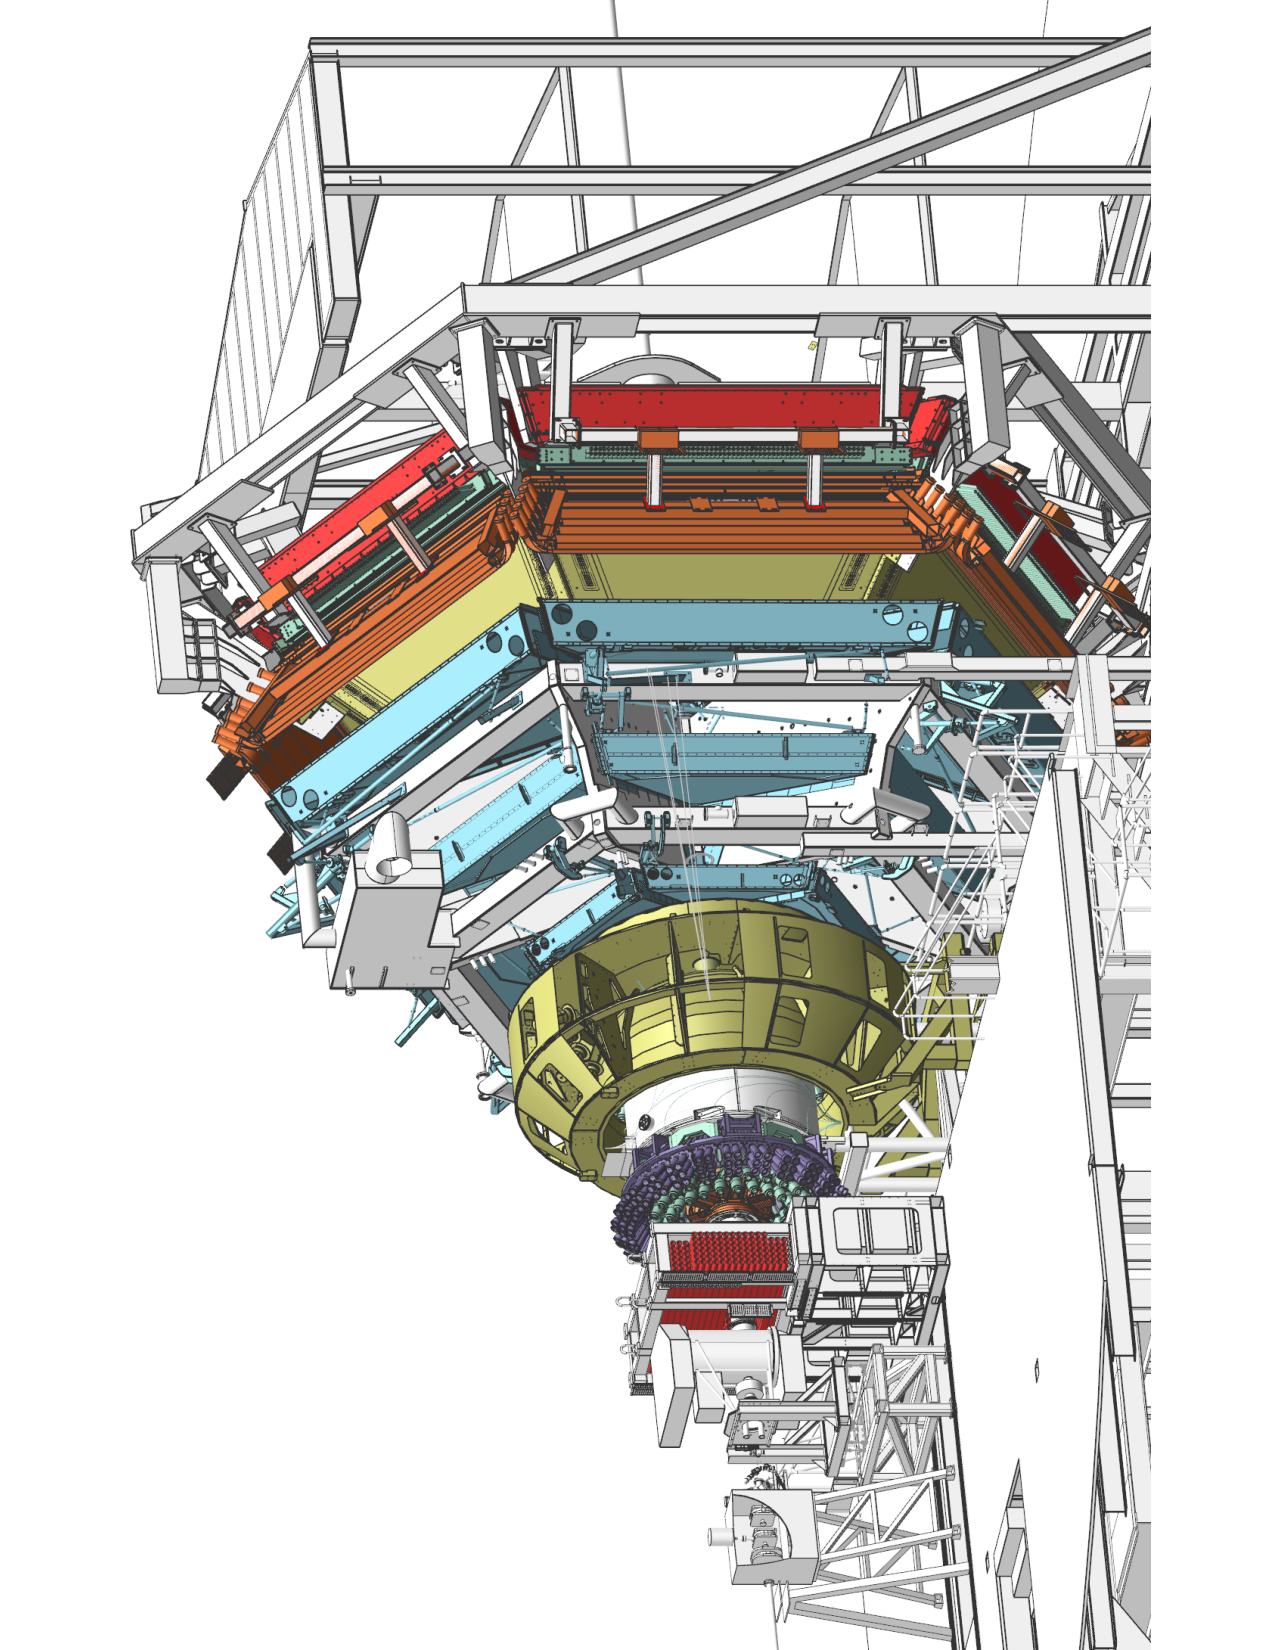
\includegraphics[width=0.36\textwidth,natwidth=610,natheight=642,angle=-90]{pics/ctof_clas12.pdf}}}
\end{picture} 
\caption{Model representation of the CLAS12 spectrometer in Hall~B at Jefferson Laboratory. The
electron beam is incident from the left side of this figure. The CLAS12 detector is roughly 20~m in scale
along the beam axis. }
\label{clas12-model}
\end{figure}
%%%%%%%%%%%%%%%%%%%%%%%%%%%%%%%%%%%%%%%%%%%%%%%%%%%%%%%%%

%%%%%%%%%%%%%%%%%%%%%%%%%%%%%%%%%%%%%%%%%%%%%%%%%%%%%%%%%
\begin{figure}[htbp]
\vspace{3.0cm}
\begin{picture}(50,50) 
\put(25,132)
{\hbox{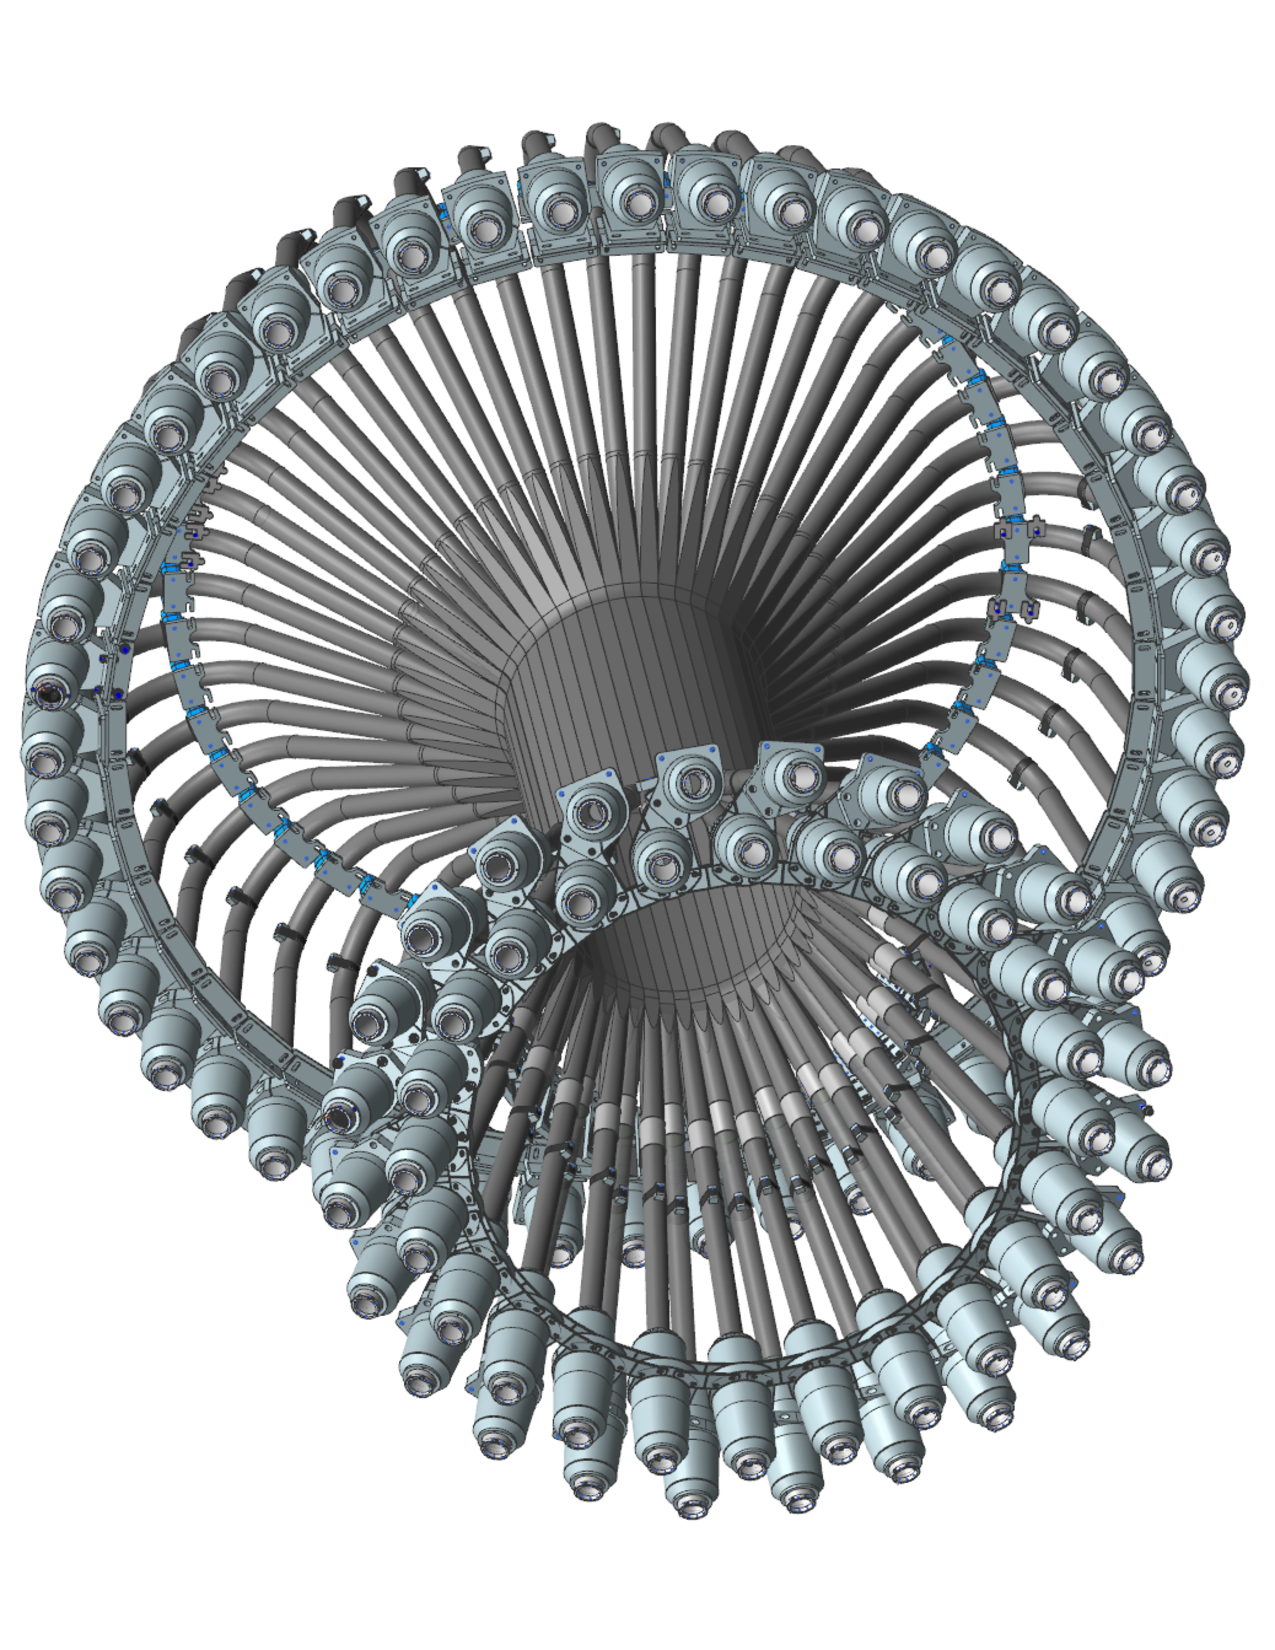
\includegraphics[width=0.30\textwidth,natwidth=610,natheight=642,angle=-90]{pics/ctof-design.pdf}}}
\end{picture} 
\caption{View of CTOF system for CLAS12. The scintillation bars form a hermetic barrel and the PMTs are
read out at the ends of long light guides attached to each end of the bars. The beam enters the detector in
this figure from the left side along the symmetry axis of the barrel.} 
\label{ctof-design}
\end{figure}
%%%%%%%%%%%%%%%%%%%%%%%%%%%%%%%%%%%%%%%%%%%%%%%%%%%%%%%%%

This paper focuses on the CLAS12 CTOF detector system and is organized as follows:
Section~\ref{sec:overview} provides a high-level overview of the CTOF system and its design
requirements, Section~\ref{sec:design} provides a technical description of the system design, and
Section~\ref{sec:performance} highlights the performance of the system through bench testing with
cosmic rays, as well as during the 2017 beam commissioning run and 2018 data runs. Finally,
Section~\ref{sec:summary} provides a summary regarding the CTOF detector system for CLAS12.

\section{Overview of the CTOF System}
\label{sec:overview}

The CTOF system specifications call for an average effective time resolution for each counter $\sigma_{TOF}$
along its full length of 80~ps. The CTOF detector surrounds the experimental target at a radial distance of
25~cm and consists of 48 90-cm-long scintillation bars having a trapezoidal cross section to form a hermetic
barrel as shown in Fig.~\ref{ctof-design}. The barrel is positioned inside the solenoid magnet just inside of
the CND and just outside of the central tracking system as shown in Fig.~\ref{cut-view}. This figure shows
that the CTOF is mounted to the solenoid with the beamline along the symmetry axis of its barrel. A summary
of the CTOF technical parameters is given in Table~\ref{spec-table}. 

%%%%%%%%%%%%%%%%%%%%%%%%%%%%%%%%%%%%%%%%%%%%%%%%%%%%%%%%%
\begin{figure}[htbp]
\vspace{2.7cm}
\begin{picture}(50,50) 
\put(-20,-41)
{\hbox{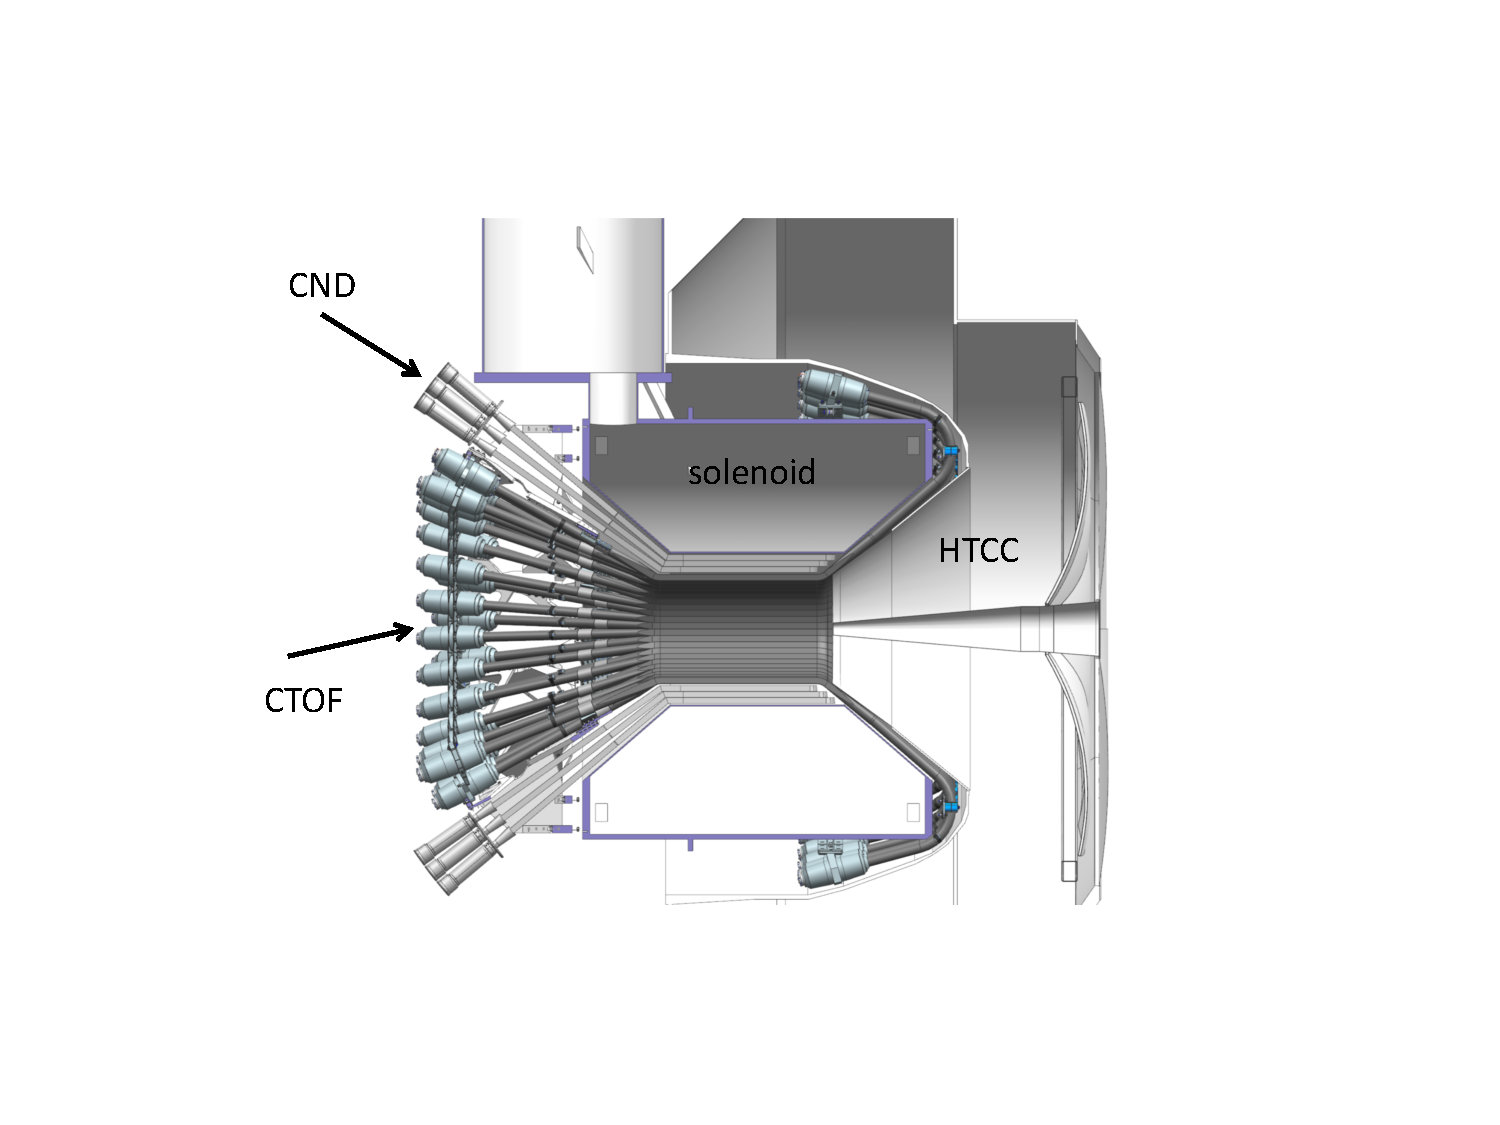
\includegraphics[width=0.50\textwidth,natwidth=610,natheight=642]{pics/ctof-insitu.pdf}}}
\end{picture} 
\caption{CTOF mounted within the CLAS12 solenoid in a cut view where the beam axis runs along the
barrel symmetry axis with the beam entering from the left. This figure shows the CTOF in relation to
the CND, the cryostat of the superconducting solenoid (outlined in purple), and the HTCC. Note that the
central tracking system, target system, and beamline elements are not shown here.}
\label{cut-view}
\end {figure}
%%%%%%%%%%%%%%%%%%%%%%%%%%%%%%%%%%%%%%%%%%%%%%%%%%%%%%%%%

Each counter is read out via a photomultiplier tube (PMT) on each end through long light guides. As shown in
Figs.~\ref{ctof-design} and \ref{cut-view}, the upstream light guides are straight and the downstream light
guides are bent to curve around the downstream face of the solenoid magnet allowing clearance for the HTCC
to be positioned just downstream of the Central Detector. The upstream light guides are 1~m long and the
downstream light guides are 1.6~m long. These lengths are necessary to position the field-sensitive PMTs in
reduced regions of the solenoid fringe field. However, even in these positions, the PMTs reside in
inhomogeneous fields as large as 1~kG (the practical limit of our magnetic shield design) at the location of the
upstream PMTs and as large as 400~G at the location of the downstream PMTs. In order to allow for operation
of the PMTs in this environment, they are mounted within multi-layer magnetic shields (see
Section~\ref{sec:shields}).

The CTOF system is necessary to identify charged particles in the CLAS12 Central Detector. Given the
time resolution of the counters, the momentum threshold for particle identification can be defined. These
thresholds are established by the 3$\sigma$ separation requirement for particle types at momenta where
identification can occur with up to an order of magnitude difference in the relative yields of the different
species. The momentum limit for particle identification is illustrated by computing the flight time
differences between different charged particle species, pions, kaons, and protons, for tracks perpendicularly
incident upon the detector assuming $\sigma_{TOF}$ = 80~ps. Figure~\ref{tdiff} shows the computed flight
time differences as a function of momentum. Where the 3$\sigma$ line crosses the computed time difference
curves defines the momentum limit for particle identification for each particle species. These limits are given
as 0.58~GeV for $\pi/K$ separation, 0.93~GeV for $K/p$ separation, and 1.14~GeV for $\pi/p$ separation
(see Table~\ref{spec-table}). The minimum momentum acceptance for CTOF is roughly 300~MeV as lower
momentum tracks are curled up in the solenoid field and never reach the inner surface of the CTOF counters.

%%%%%%%%%%%%%%%%%%%%%%%%%%%%%%%%%%%%%%%%%%%%%%%%%%%%%%%%%
\begin{figure}[htbp]
\vspace{2.0cm}
\begin{picture}(50,50) 
\put(7,-72)
{\hbox{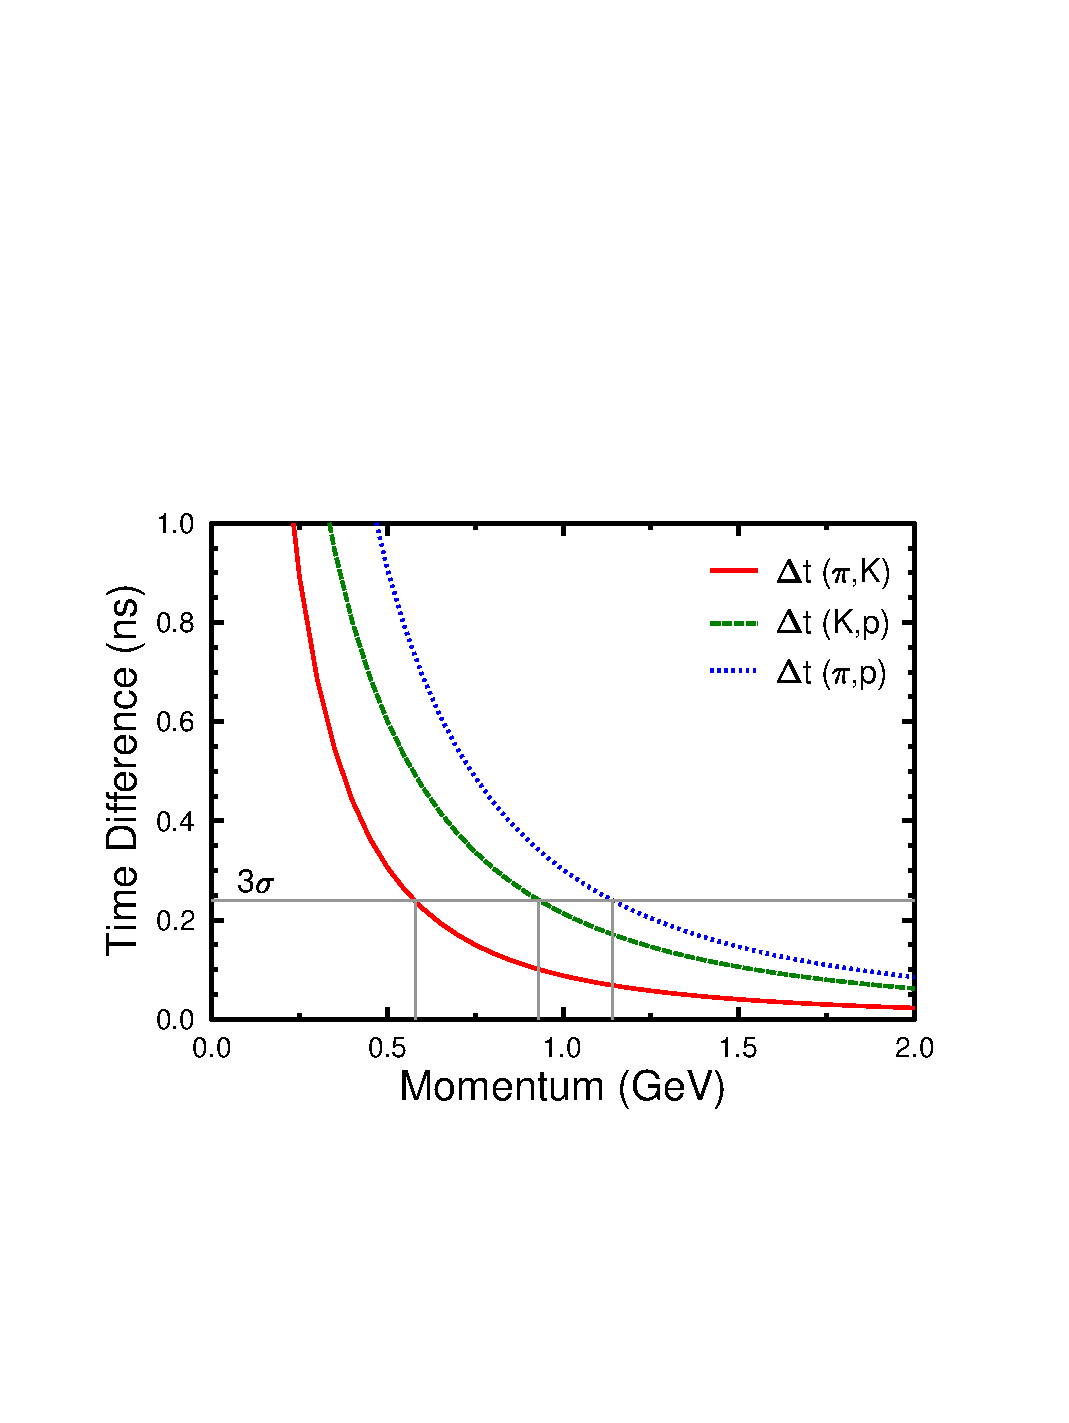
\includegraphics[width=0.55\textwidth,natwidth=610,natheight=642]{pics/tdiff_alt.pdf}}}
\end{picture} 
\caption{Flight time differences (ns) between protons and pions, between protons and kaons, and between
kaons and pions (as indicated) for a 25~cm path length from the target to the CTOF system plotted vs.
particle momentum (GeV). The horizontal line indicates a time difference three times larger than the
average CTOF counter design resolution of $\sigma_{TOF}$ = 80~ps. The vertical lines that meet each
curve represent the momentum limit for 3$\sigma$ particle species separation. The minimum momentum
for tracks to reach the CTOF system is roughly 300~MeV.}
\label{tdiff}
\end{figure}
%%%%%%%%%%%%%%%%%%%%%%%%%%%%%%%%%%%%%%%%%%%%%%%%%%%%%%%%%

Figure~\ref{pth-kin} shows a plot of the momentum versus polar angle for charged pions in CLAS12
from data of a 10.6~GeV electron beam incident upon a liquid-hydrogen target. Here it is seen that
the typical track momenta accepted by CTOF are in the range below 2~GeV.

%%%%%%%%%%%%%%%%%%%%%%%%%%%%%%%%%%%%%%%%%%%%%%%%%%%%%%%%%
\begin{figure}[htbp]
\vspace{3.2cm}
\begin{picture}(50,50) 
\put(25,-47)
{\hbox{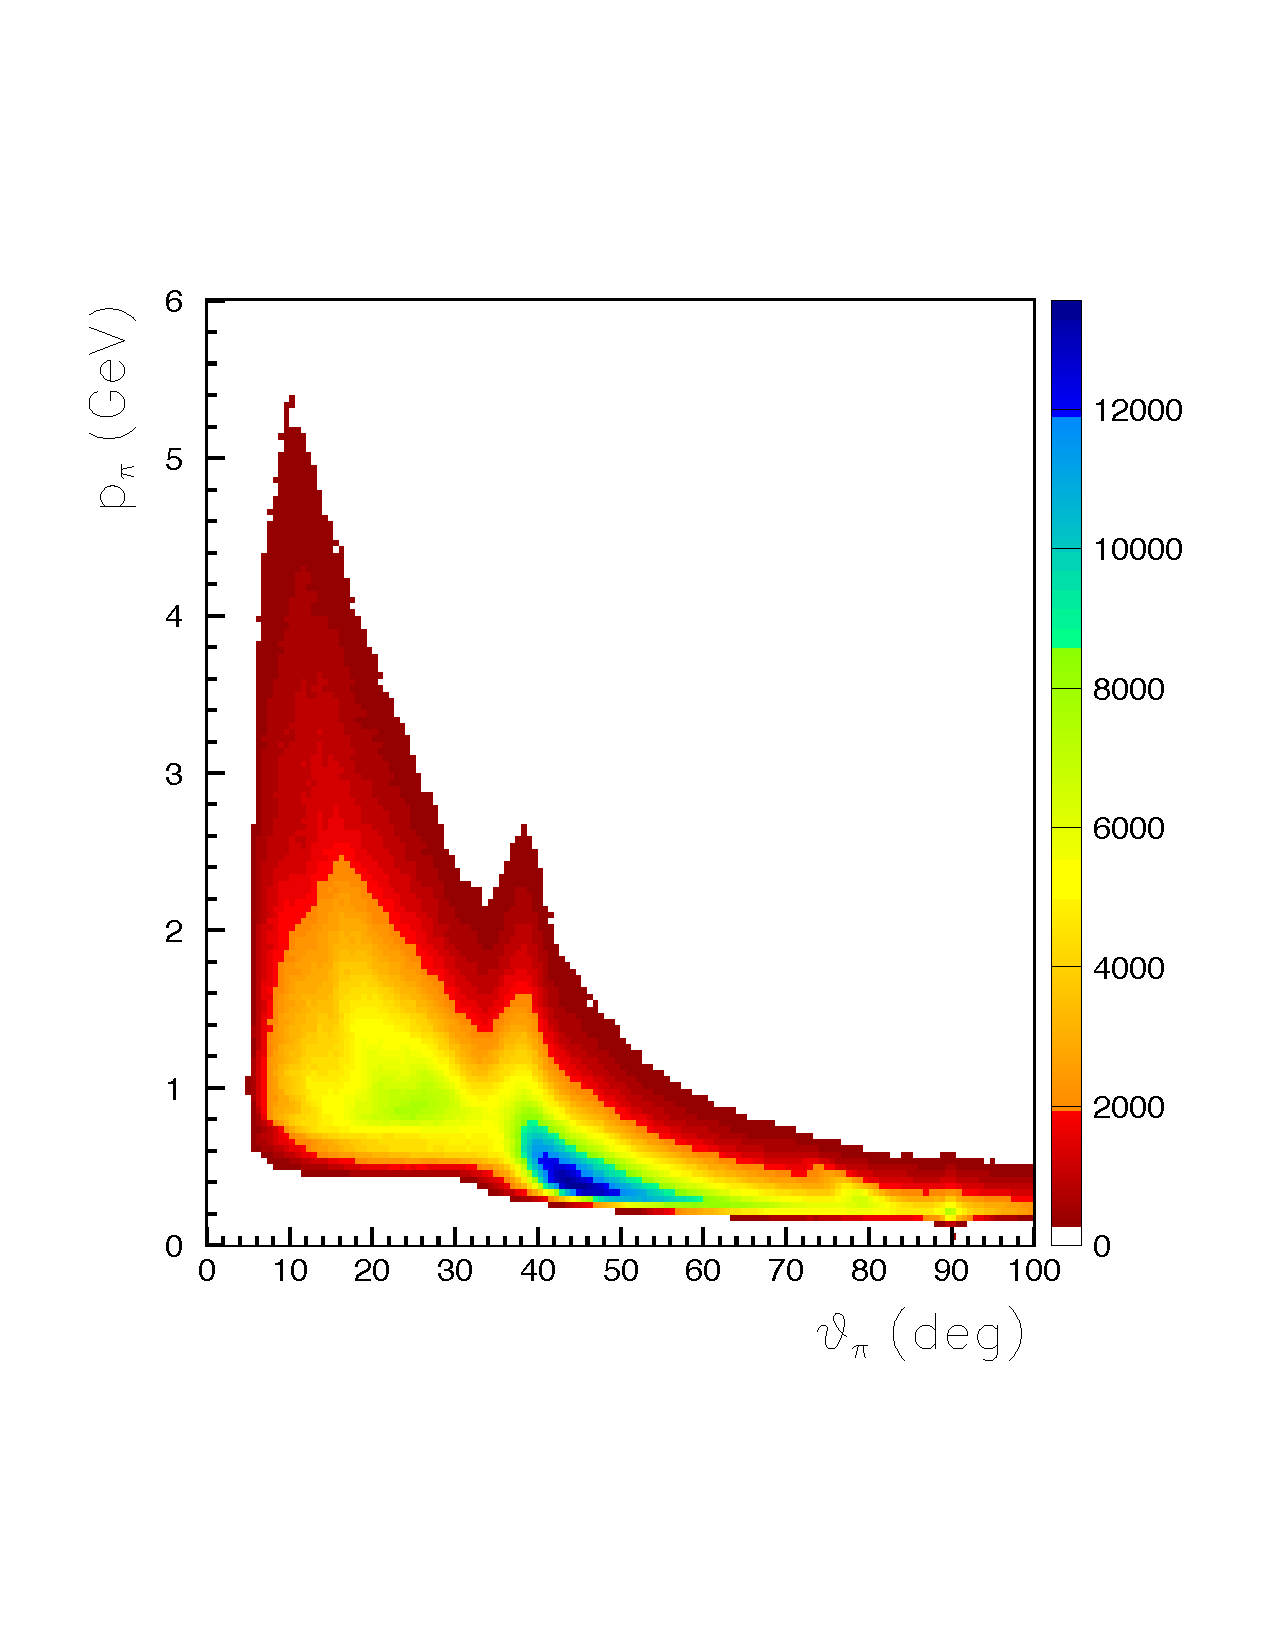
\includegraphics[width=0.37\textwidth,natwidth=610,natheight=642]{pics/pthpi.pdf}}}
\end{picture} 
\caption{Momentum (GeV) vs. polar angle (deg) for charged pions in CLAS12 from beam data for a 10.6~GeV
electron beam incident upon a liquid-hydrogen target. The discontinuity at $\theta=35^\circ$ is due to the
small acceptance gap between the Forward and Central Detectors.}
\label{pth-kin}
\end{figure}
%%%%%%%%%%%%%%%%%%%%%%%%%%%%%%%%%%%%%%%%%%%%%%%%%%%%%%%%%

The scintillation counter signals are used in the CLAS12 Level~1 trigger~\cite{trigger-nim} to define
charged hadrons in the Central Detector, as well as to provide an effective charged particle veto for
the CND. The CTOF system must, therefore, provide signals representing a uniform response with
adequate granularity. The pulse height information is also used for energy-loss measurements to provide
a supplemental means for the identification of slow particles.

%%%%%%%%%%%%%%%%%%%%%%%%%%%%%%%%%%%%%%%%%%%%%%%%%%%%%%%%%
\begin{table*}[ht]
\begin{center}
\begin{tabular} {l|l} \hline
~~Parameter~~ &~~~~~~~~~~~~~~~~~~~~~~ Design Value ~~~~~~~~~~\\ \hline
Counters             & Barrel of 48 EJ-200 bars; double-ended readout \\
Angular Coverage     & $\theta$: (35$^\circ$,125$^\circ$), $\phi$: (-180$^\circ$,180$^\circ$) \\
Counter Dimensions   & Trapezoidal cross section $\sim 3.4 \times 3.0 \times 90$~cm$^3$ \\
PMTs                 & Hamamatsu R2083 (H2431-MOD assembly)    \\
Upstr. Light Guides  & O.D.=5.08~cm, 1~m long, focusing design, straight \\
Dnstr. Light Guides  & O.D.=5.08~cm, 1.6~m long, focusing design, bent 135$^\circ$ \\
Magnetic Shields     & 3 ferromagnetic layers with inner compensation coils \\
Time Resolution    & 65~ps (intrinsic) / 80~ps (effective) \\
$\pi$/$K$ separation & 3$\sigma$ up to 0.58~GeV \\ 
$K$/$p$ separation   & 3$\sigma$ up to 0.93~GeV \\ 
$\pi$/$p$ separation & 3$\sigma$ up to 1.14~GeV \\ \hline
\end{tabular}
\end{center}
\caption{CTOF technical design parameters.}
\label{spec-table}
\end{table*}
%%%%%%%%%%%%%%%%%%%%%%%%%%%%%%%%%%%%%%%%%%%%%%%%%%%%%%%%%

With a solenoid diameter of 100~cm, the thickness of the CTOF scintillation bars was limited to $\sim$3~cm
given the constraints imposed by the other Central Detector subsystems. In order to accommodate the target
and the central tracking system, the CTOF was positioned at a radius from the beamline of 25~cm. To ensure
maximal $\phi$ acceptance, the individual CTOF counters have a wedge-shaped geometry to form a hermetic
barrel. The width of the counters of $\sim$3.4~cm was selected to ensure that the maximum count rates do
not exceed 500~kHz per counter with the solenoid at its nominal full field and a beam-target luminosity of
1$\times$10$^{35}$~cm$^{-2}$s$^{-1}$.

\section{Design of the CTOF System}
\label{sec:design}

The intrinsic time resolution of the counters is determined mainly by the number of photons created in the
scintillation bar by passing charged particles that ultimately propagate to the photocathodes of the PMTs.
Due to the geometry of the scintillation bar and the light guides, there are attenuation losses of the created
light. As well, the photons that propagate to the PMTs are dispersed in time via the different paths that they
travel. The response of the PMT, including variations in response across the photocathode, causes further
dispersion of the times of the created photoelectrons reaching the accelerating structure of the PMT. Each
of these effects must be folded in with the additional signal dispersion induced along the accelerating structure
of the PMT. These contributions determine the intrinsic time resolution of the counter assembly. For our
purposes we also include in the accounting of the intrinsic time resolution effects from signal dispersion along
the readout signal cables and the resolution smearing of the readout electronics. These resolutions were
determined during our bench test measurements detailed in Section~\ref{sec:bench}. However, the overall
effective resolution of the system also includes additional smearing effects from other CLAS12 subsystems
that are required as input to calibrate the CTOF response. This includes the determination of the track path
length and reaction vertex point from the central tracking reconstruction and the event start time from the
Forward Detector. It also includes positional offsets and distortions of the installed detectors relative to their
ideal geometries and differences in the true solenoid magnetic field from what is used in event reconstruction.
The effective counter time resolutions determined during beam studies in CLAS12 are detailed in
Section~\ref{tres-beam}. Table~\ref{spec-table} therefore includes two measures of the CTOF design time
resolution. The value of 65~ps is our requirement for the intrinsic time resolution and 80~ps represents the
overall effective resolution that sets the 3$\sigma$ specifications for particle identification.

Studies of prototype counters for the CTOF system with 1-m long scintillation bars of cross sections 3~cm
$\times$ 3~cm, readout through long light guides, showed that the ultimate counter time resolution could be
achieved only after careful optimization of the overall system design~\cite{baturin-2009}. In this section the
design details of the scintillation bars, the light guides, the magnetic shields, and the electronics are discussed.
Each component of the system design was considered within the context of the design constraints both for the
CTOF and the neighboring detector subsystems, and optimized against cost and performance considerations. 

\subsection{Geometry}
\label{geometry}

The scintillation bars of the CTOF barrel are composed of two slightly different designs that alternate in
azimuth. A pair of neighboring counters is shown in Fig.~\ref{counter-pair}. The difference between the two
designs is in the upstream straight light guide and the upstream end of the scintillation bars where they
attach to the light guide. This design is necessary to allow for sufficient spacing for the bulky magnetic
shields and their associated support structure. The downstream elements of the design are identical for all
counters.

%%%%%%%%%%%%%%%%%%%%%%%%%%%%%%%%%%%%%%%%%%%%%%%%%%%%%%%%%
\begin{figure}[htbp]
\vspace{1.7cm}
\begin{picture}(50,50) 
\put(10,108)
{\hbox{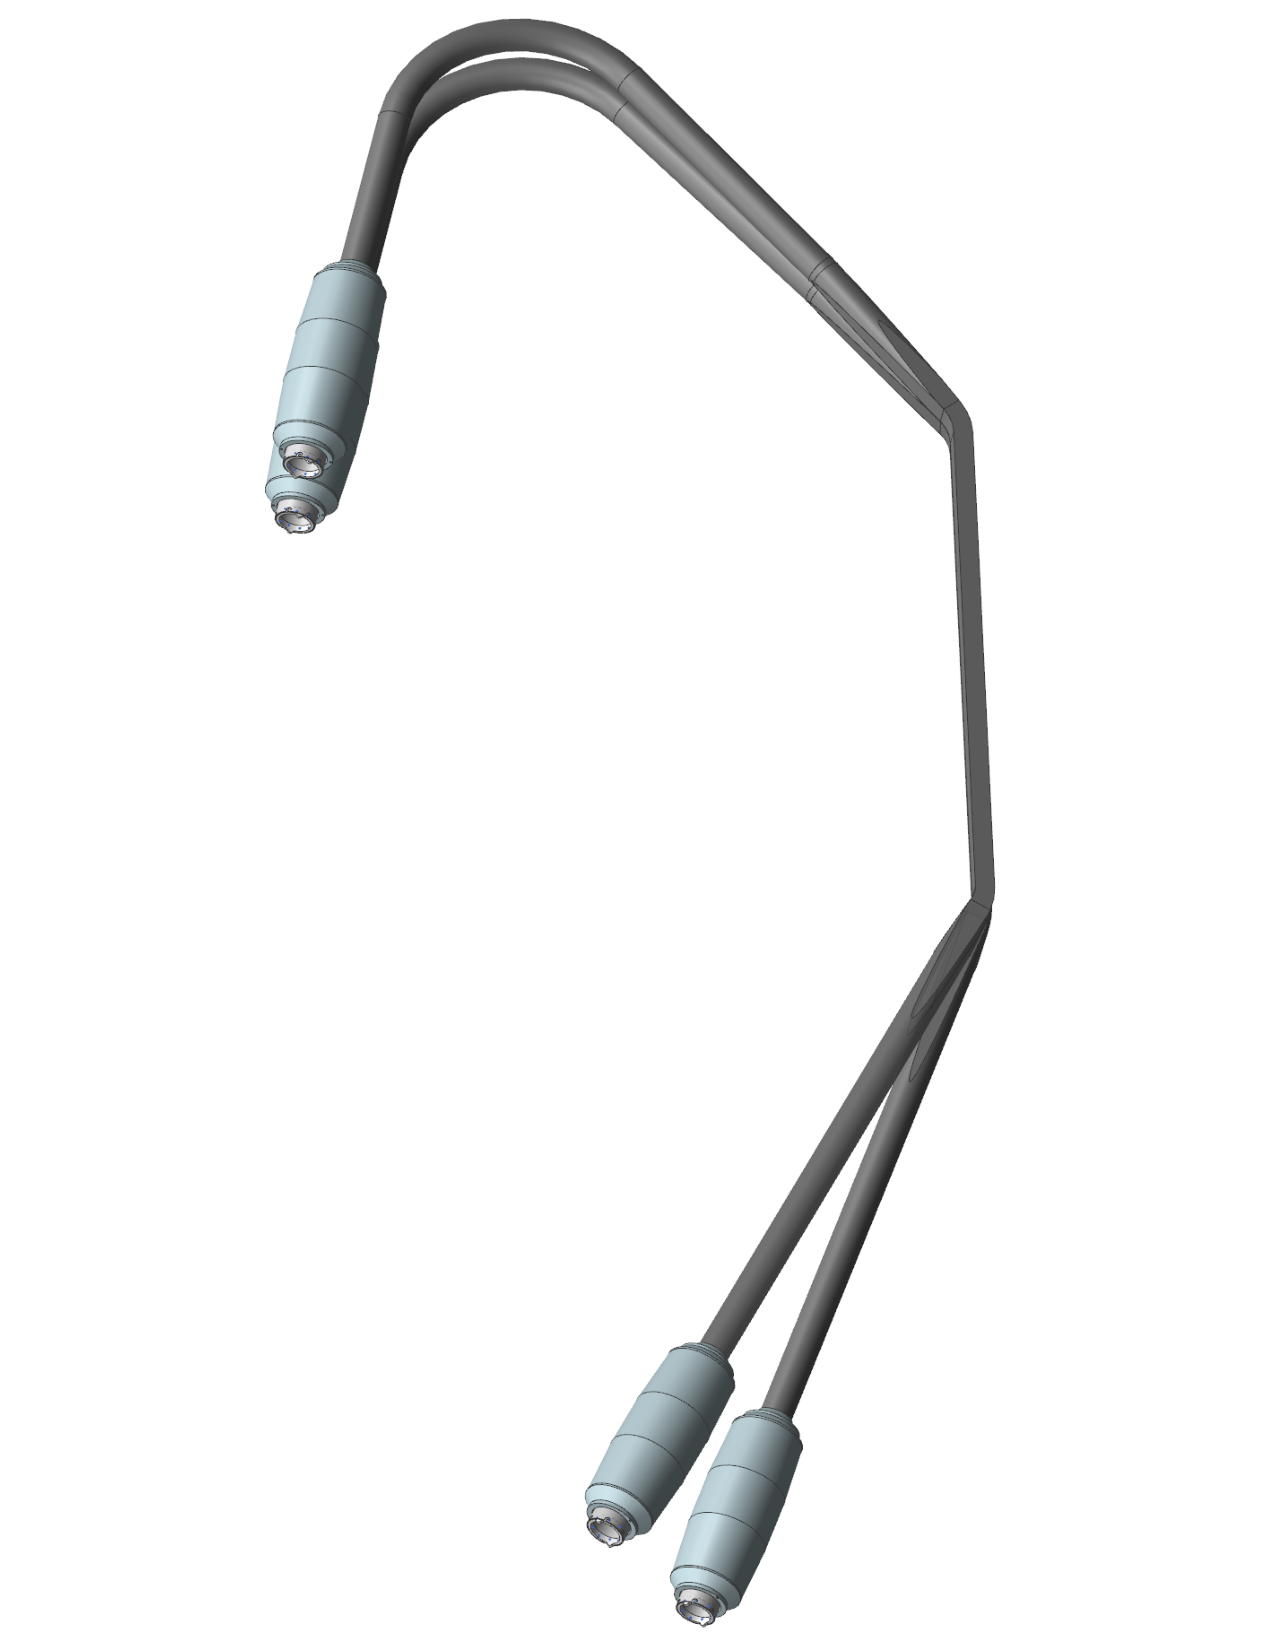
\includegraphics[angle=-90,width=0.32\textwidth,natwidth=610,natheight=642]{pics/counter-pair.pdf}}}
\end{picture} 
\caption{A pair of neighboring CTOF counters with two slightly different designs for the upstream light
guide and the upstream end of the scintillation bars.} 
\label{counter-pair}
\end{figure}
%%%%%%%%%%%%%%%%%%%%%%%%%%%%%%%%%%%%%%%%%%%%%%%%%%%%%%%%%

The two different CTOF counter designs have a slightly different pitch angle for the scintillation bars on
the upstream side. The ``low-pitch'' design has a pitch angle of 21.8$^\circ$ and the ``high-pitch'' design
has a pitch angle of 29.1$^\circ$. For all scintillation bars, however, the pitch angle at the downstream end
is 36.0$^\circ$. Figure~\ref{scint-geom} shows a schematic side view and end view of a ``generic''
scintillation bar.

%%%%%%%%%%%%%%%%%%%%%%%%%%%%%%%%%%%%%%%%%%%%%%%%%%%%%%%%%
\begin{figure}[htbp]
\vspace{3.2cm}
\begin{picture}(50,50) 
\put(3,190)
{\hbox{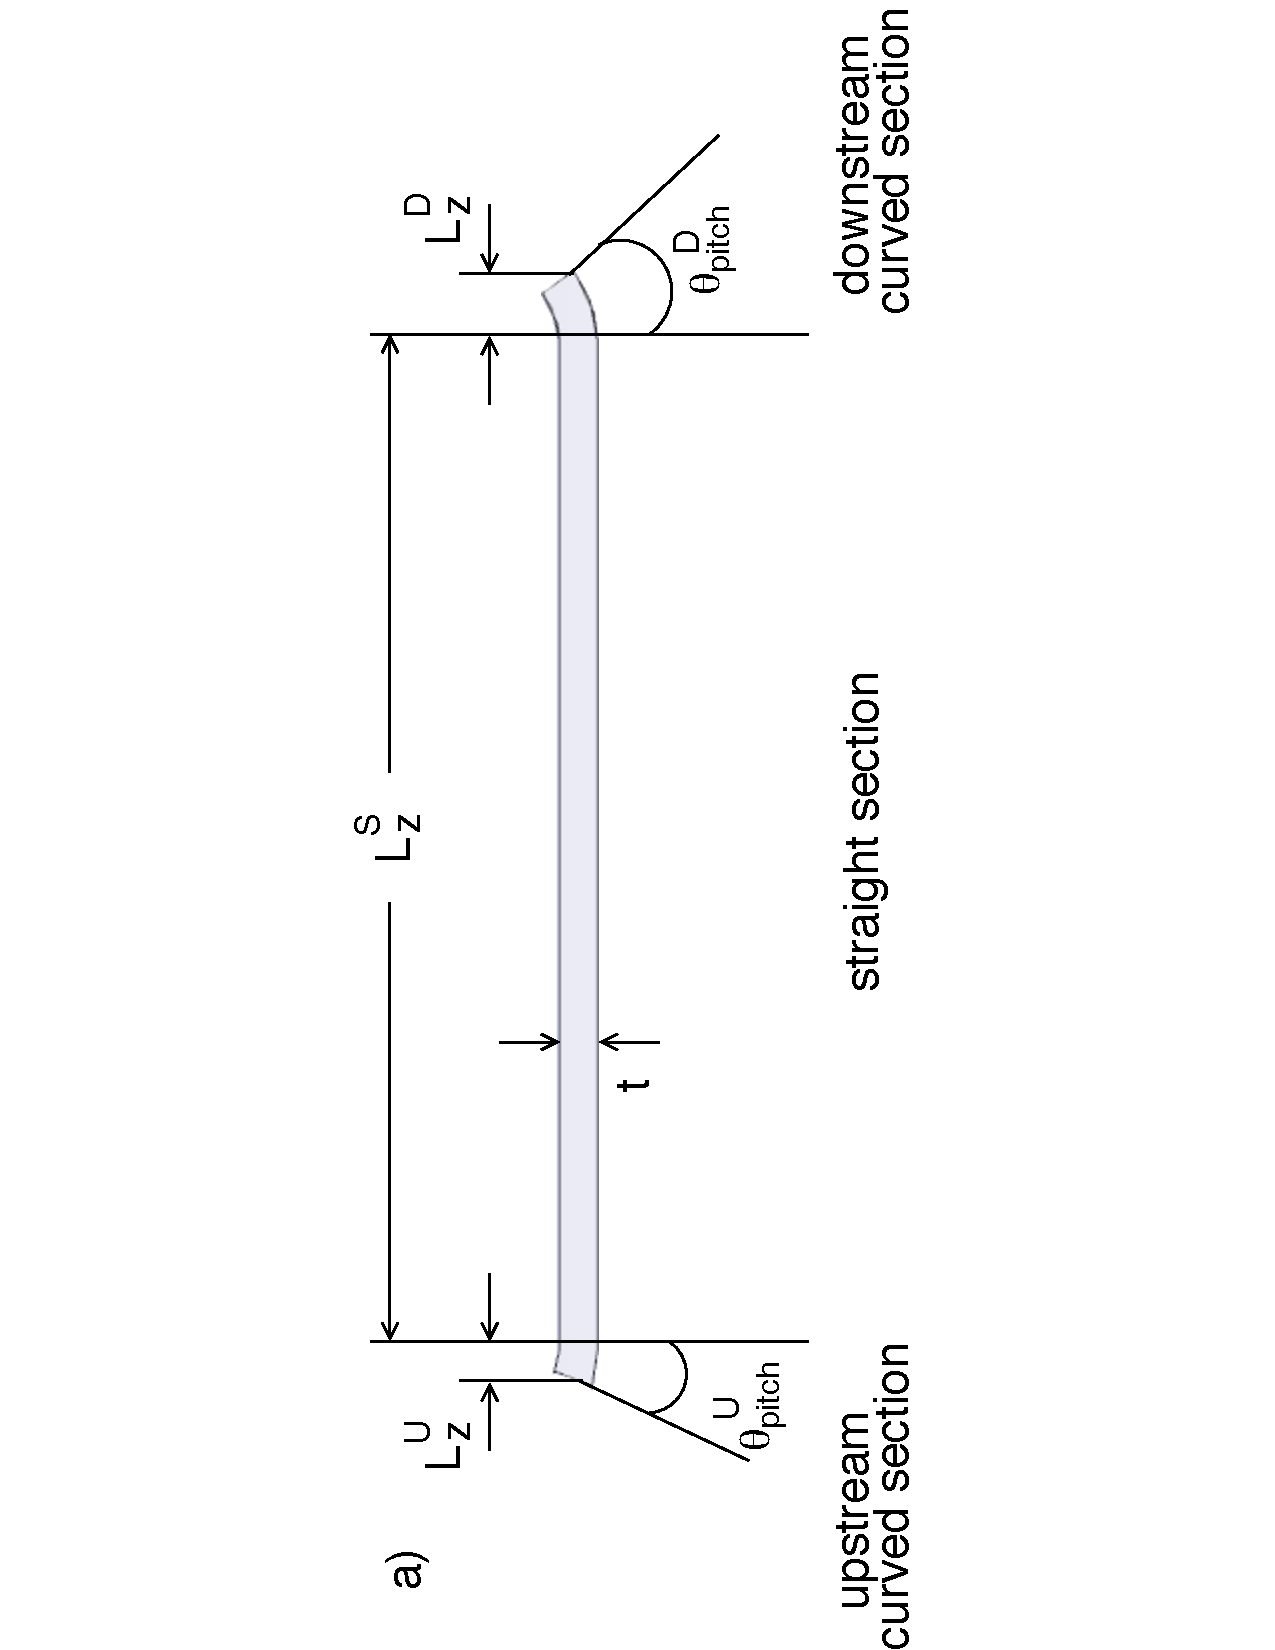
\includegraphics[angle=-90,width=0.38\textwidth,natwidth=610,natheight=642]{pics/scint-geom-a.pdf}}}
\put(55,-30)
{\hbox{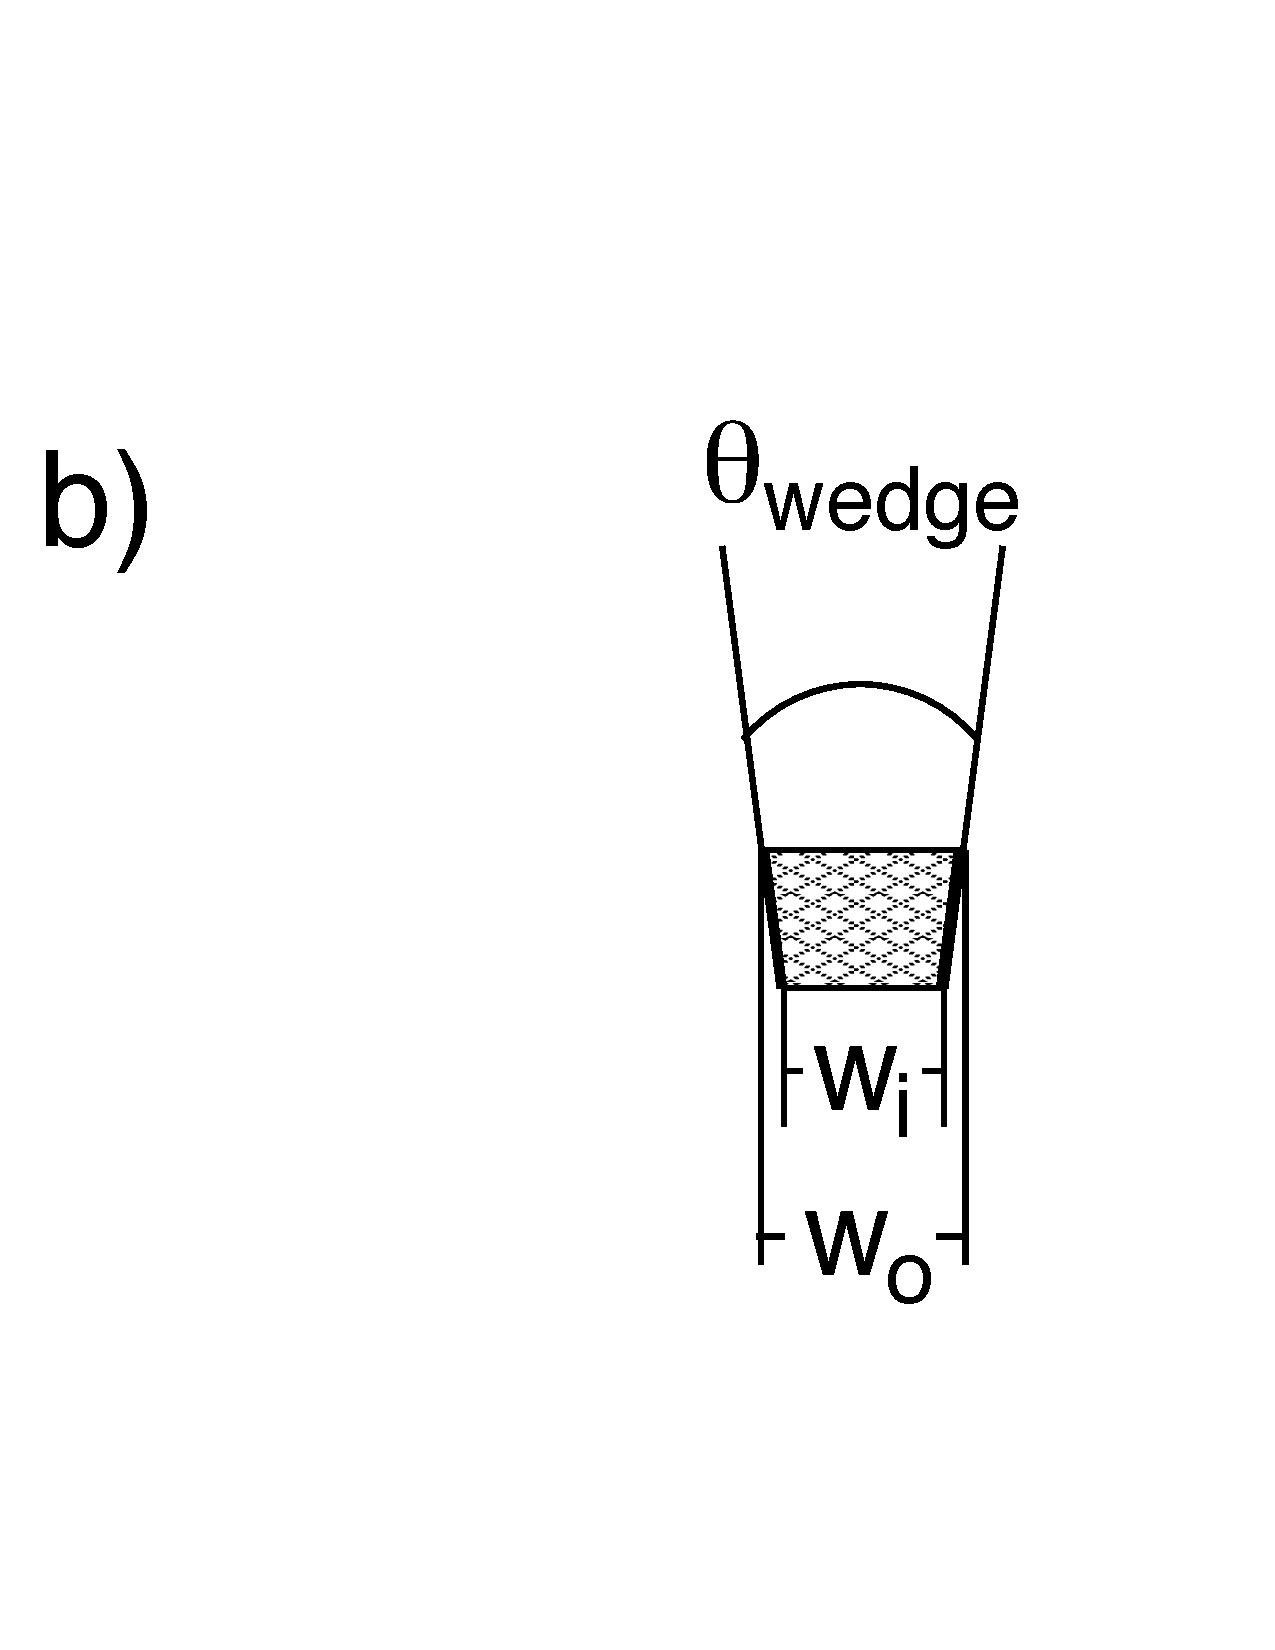
\includegraphics[angle=-90,width=0.20\textwidth,natwidth=610,natheight=642,angle=90]
{pics/scint-geom-b.pdf}}}
\end{picture} 
\caption{Schematic views of a generic CTOF scintillation bar showing a) a side view and b) an end view. The
parameters used to define the geometry of the bar are listed. See Table~\ref{bar-geom} for the detailed
specifications.}
\label{scint-geom}
\end{figure}
%%%%%%%%%%%%%%%%%%%%%%%%%%%%%%%%%%%%%%%%%%%%%%%%%%%%%%%%%

The scintillation bar design is essentially a uniform wedge-shaped piece of scintillation material that
subtends a 7.5$^\circ$ azimuthal range as seen from the target. The very ends of the bars curve upwards
to join the light guides. A simplified description of the two different CTOF scintillation bar designs is given
in Table~\ref{bar-geom} using the variables defined in Fig.~\ref{scint-geom}. Here $L_z$ is the section
length along the beam/$z$-axis, $w_i$ ($w_o$) is the width of the scintillation bar at its inside (outside)
face, and $\theta_{wedge}$ is the azimuthal angle subtended by each bar as seen from the target. Note that
the bars do not have a uniform wedge-shaped cross section from end to end. The upstream and downstream
curved sections have a slightly projective geometry to maximize the surface area for light transmission.
However the bars always fit within a 7.5$^\circ$ azimuthal wedge from the target. The surface area of the
ends of each counter element $A_{end}$ is listed in Table~\ref{bar-geom}. A more complete description of
the counter geometry is given in Ref.~\cite{geom-note}.

%%%%%%%%%%%%%%%%%%%%%%%%%%%%%%%%%%%%%%%%%%%%%%%%%%%%%%%%%
\begin{table*}[ht]
\begin{center}
\begin{tabular} {c|r|cc} \hline
Section       & Parameter          & \multicolumn{2}{c}{Design Value} \\ \hline
              &                    & Low-Pitch Angle & High-Pitch Angle \\ \cline{3-4}
Upstream      & $L_z^U$            & 2.924~cm  & 4.125~cm	  \\
              & $\theta_{pitch}^U$ & 21.8$^\circ$ & 29.1$^\circ$ \\
              & $A_{end}$          & 11.20~cm$^2$ & 12.13~cm$^2$ \\ \hline
Straight      & $L_z^S$            & \multicolumn{2}{c}{80.683~cm}    \\
              & $A_{end}$          & \multicolumn{2}{c}{10.32~cm$^2$} \\ \hline
Downstream    & $L_z^D$            & \multicolumn{2}{c}{5.624~cm}     \\
              & $\theta_{pitch}^D$ & \multicolumn{2}{c}{36.0$^\circ$} \\
              & $A_{end}$          & \multicolumn{2}{c}{11.02~cm$^2$} \\ \hline
Scintillation & $w_i$              & \multicolumn{2}{c}{3.211~cm}     \\ 
Bar           & $w_o$              & \multicolumn{2}{c}{3.607~cm}     \\  
              & $\theta_{wedge}$   & \multicolumn{2}{c}{7.5$^\circ$}  \\ 
              & $t$                & \multicolumn{2}{c}{3.022~cm}  \\ \hline   
\end{tabular}
\end{center}
\caption{Geometry specifications for the CTOF scintillation bars. See Fig.~\ref{scint-geom} for
details on the definitions of the parameters.}
\label{bar-geom}
\end{table*}
%%%%%%%%%%%%%%%%%%%%%%%%%%%%%%%%%%%%%%%%%%%%%%%%%%%%%%%%%

\subsection{Scintillation Material}
\label{scint-mat}

To optimize the time resolution for the CTOF system, the scintillation bars were required to provide a
fast time response with low light attenuation. For this application EJ-200 plastic scintillator from Eljen
was selected. This material has the same technical specifications as for BC-408 by Bicron. EJ-200 uses
polyvinyltoluene as its base polymer. The characteristics of this material are detailed in
Table~\ref{ej200-specs}.

%%%%%%%%%%%%%%%%%%%%%%%%%%%%%%%%%%%%%%%%%%%%%%%%%%%%%%%%%
\begin{table*}[htbp]
\begin{center}
\begin{tabular}{l|c} \hline
Light Output                  & 64\% anthracene \\
Wavelength of Max. Emission~~ & 425 nm \\
Rise Time                     & 0.9 ns \\
Decay Time                    & 2.1 ns \\
Pulse Width                   & 2.5 ns (FWHM) \\
Density                       & 1.023 g/cm$^3$ \\
Bulk Attenuation Length       & 380~cm \\
Refractive index              & 1.58 \\ \hline 
\end{tabular}
\end{center}
\caption{The properties of the plastic scintillator EJ-200~\cite{eljen-ref} used for the CTOF scintillation
bars.}
\label{ej200-specs}
\end{table*}
%%%%%%%%%%%%%%%%%%%%%%%%%%%%%%%%%%%%%%%%%%%%%%%%%%%%%%%%%

The attenuation length of a scintillation material represents the distance $\lambda$ into the material
where the probability that the photon has been absorbed is $1/e$.  The bulk attenuation length of EJ-200
is stated by its manufacturer to be $\sim$4~m. However, the practical attenuation length of the prepared
bars is smaller than this bulk value as the path length of photons from the charged particle intersection
point to the ends of the bar is increased due to the finite geometry of the bar. This practical attenuation
length should be longer than the bar to ensure sufficient photon statistics at its ends. For the CTOF bars,
the manufacturing specification was that the practical attenuation length be longer than 280~cm.
Measurements of the practical attenuation length of the CTOF counters, which include the light guides,
see Section~\ref{sec:attlen} for details, are reduced from this value by a factor of two.

The scintillation bars were required to be clear and free of visual inclusions, air bubbles, and cracks. The
bars were machined with diamond-tooled end mills on two faces and were cast against glass on the other
two faces. Upon delivery the bars were subjected to additional hand polishing to further improve the
surface quality in some cases. The polishing generally followed the guidelines recommended by Eljen
\cite{eljen-guide}. Care was taken in all phases of handling the bars to wear gloves and to avoid contact
with alcohols or other solvents.

\subsection{Light Guides}

The locations of the upstream and downstream PMTs for the CTOF system are tightly constrained by the
layout of the CLAS12 Central Detector. The upstream light guides were required to be $\sim$1~m long and
project away from the beamline in the angular range from 20$^\circ$ to 30$^\circ$. The downstream light
guides were required to wrap around the downstream face of the solenoid magnet with a length of
$\sim$1.6~m. For both light guides, the overall design principle was to ensure that they were as short as
possible to optimize the light transmittance and thus optimize the counter time resolution.

%%%%%%%%%%%%%%%%%%%%%%%%%%%%%%%%%%%%%%%%%%%%%%%%%%%%%%%%%
\begin{figure}[htbp]
\vspace{1.4cm}
\begin{picture}(50,50) 
\put(-5,90)
{\hbox{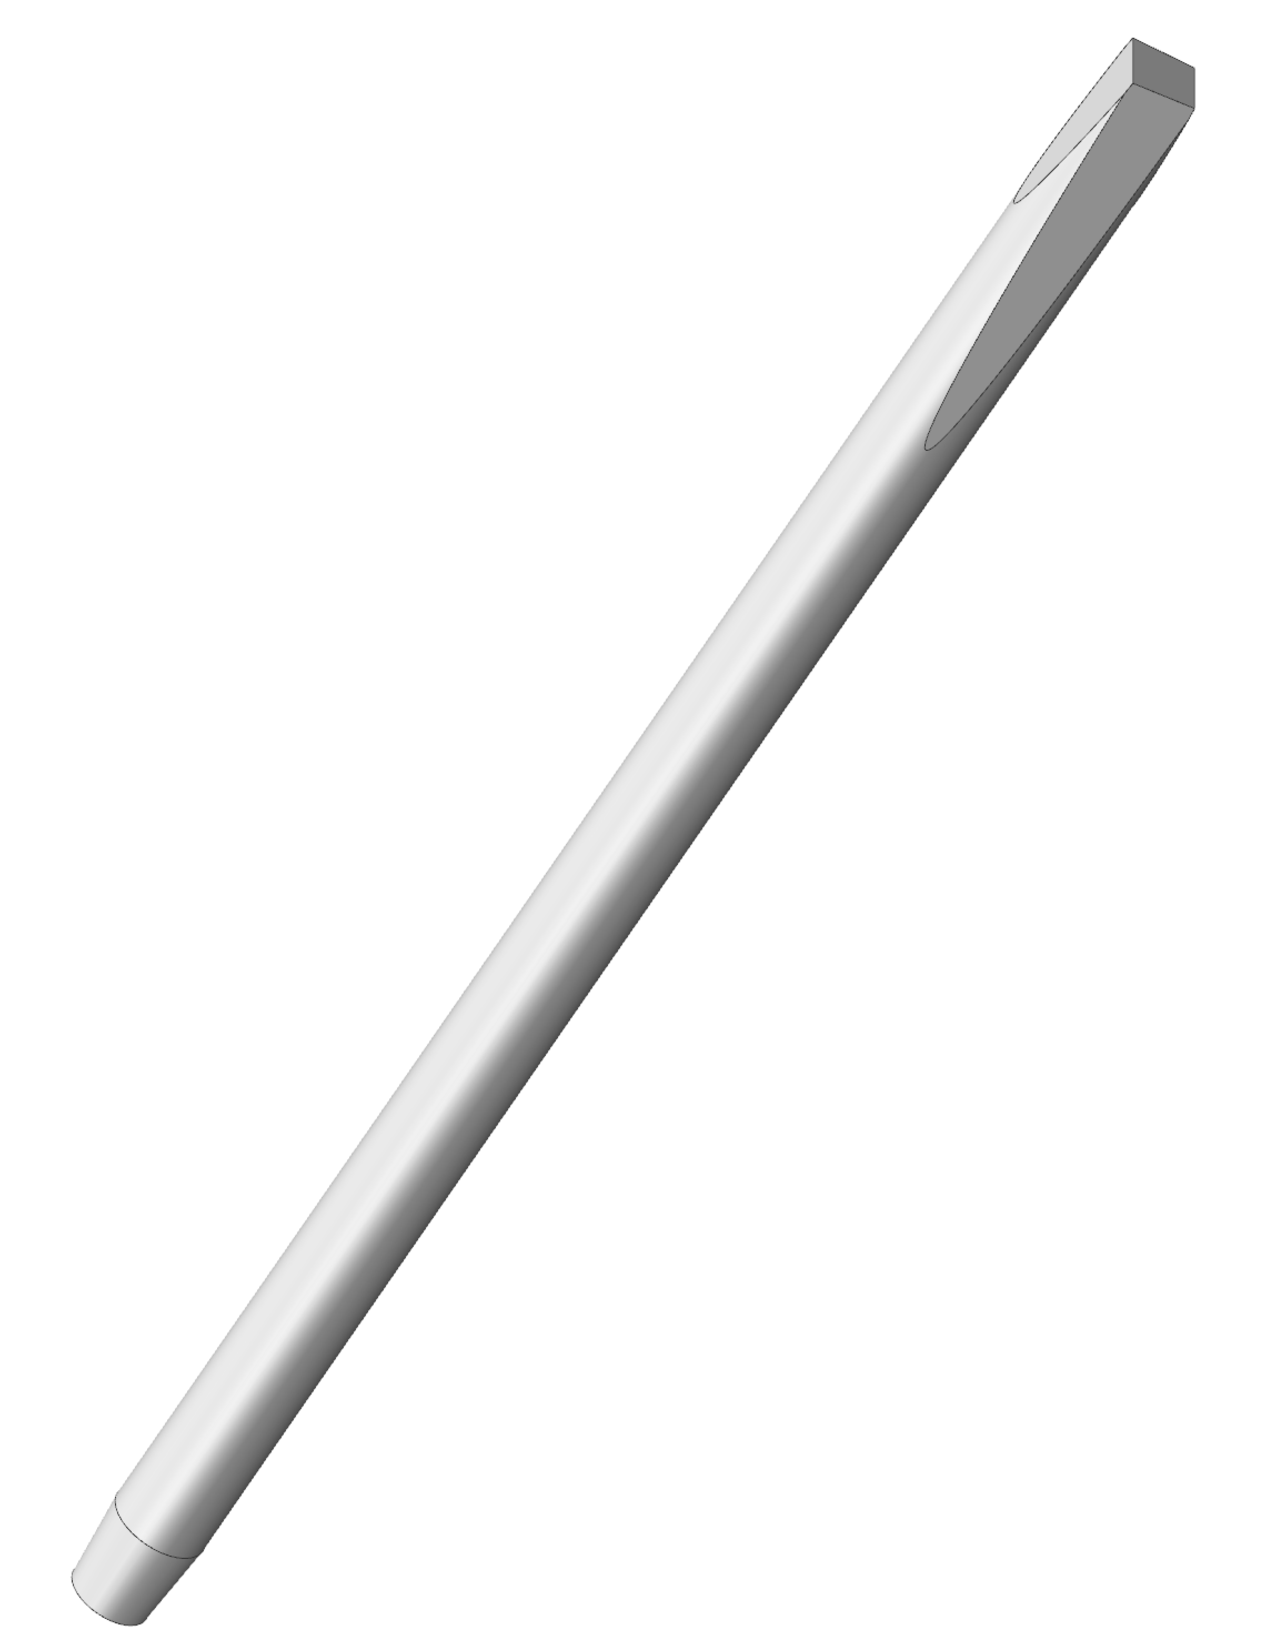
\includegraphics[width=0.18\textwidth,natwidth=610,natheight=642,angle=-95]{pics/ctof-lgu.pdf}}}
\put(90,80)
{\hbox{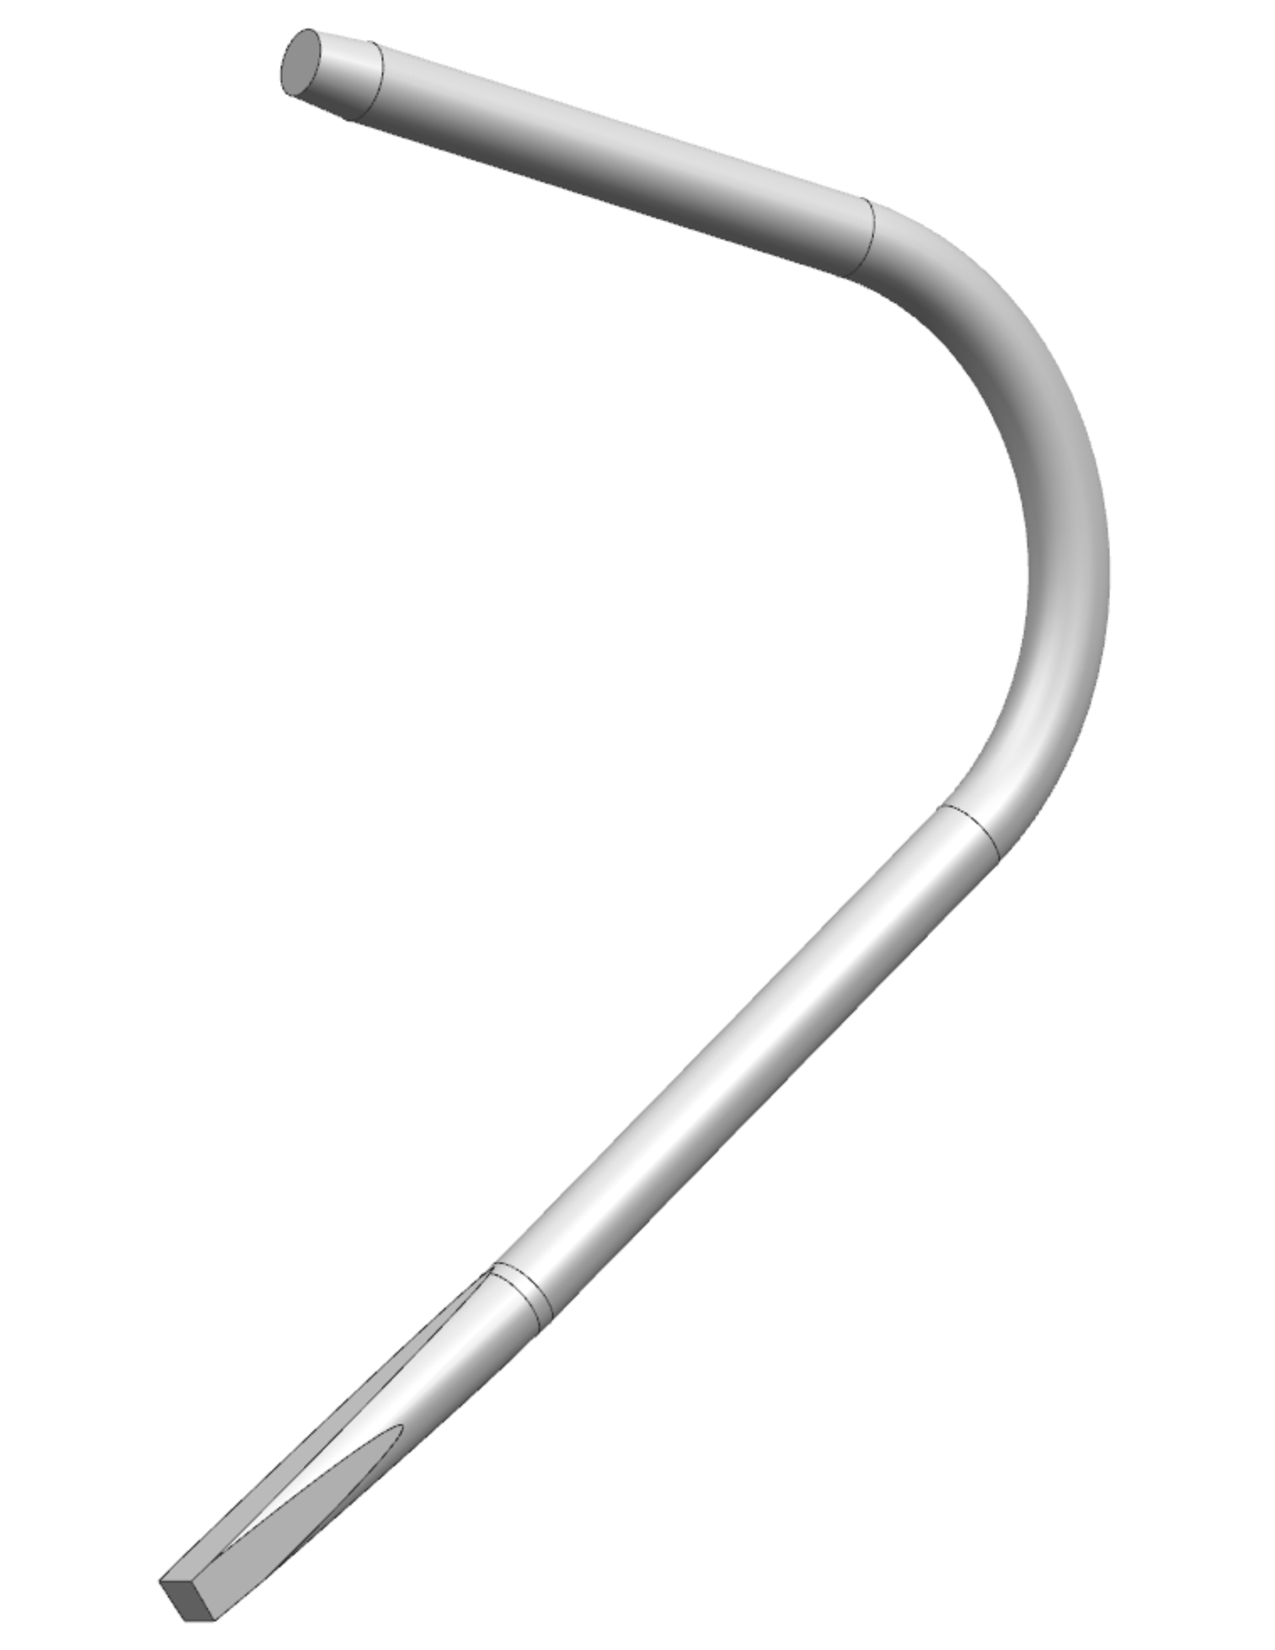
\includegraphics[width=0.20\textwidth,natwidth=610,natheight=642,angle=-80]{pics/ctof-lgd.pdf}}}
\end{picture}
\put(20,-5){(a)}
\put(140,-5){(b)}
\caption{The design of the CTOF (a) upstream and (b) downstream light guides. The wedge-shaped end
of each guide couples to the scintillation bar and the cylindrical end couples to the PMT.}
\label{ctof-lg}
\end{figure}
%%%%%%%%%%%%%%%%%%%%%%%%%%%%%%%%%%%%%%%%%%%%%%%%%%%%%%%%%

The constraints on the light guides required that they match the wedge-shaped cross section of the
scintillation bar at one end and match the circular shape of the PMT at the other end, while being restricted
to lie fully within the 7.5$^\circ$ azimuthal allotment for each of the counters. The light guides were
manufactured by Plastic-Craft Products Corporation from 5.08-cm diameter cast acrylic rods ($n$=1.49).
The downstream light guides were cast as straight rods and bent on a forming mandrel after heating in a
low-temperature oven. After the casting and machining processes, the light guides were polished to a mirror
surface at the vendor with additional polishing performed at JLab only in the case of scratches incurred
during handling.

The design of the upstream light guide is shown in Fig.~\ref{ctof-lg}(a). The sides of the acrylic
cylinder were milled to a length of 25~cm along the light guide to form a wedge up to a radius of 37~cm
in the $(r,\phi)$-plane in order to fit into the $\Delta \phi=7.5^\circ$ region. The straight cylindrical
section is 75~cm long to position the PMT in the solenoid fringe field at a position where the maximum
field is at the level of $\sim$1~kG. The design of the downstream light guide is shown in
Fig.~\ref{ctof-lg}(b). The sides of the cylinder were milled to a length of 30~cm along the light guide to
form a wedge up to a radius of 40~cm in the $(r,\phi)$ plane. The light guide bends through an angle of
135$^\circ$ over a length of 45~cm around the downstream face of the solenoid magnet to position the
downstream PMTs in a lower maximum value of the solenoid fringe field of about 400~G. 
 
\subsubsection{Monte Carlo Design Studies}
\label{lg-mc}

The light guide design was optimized using a Monte Carlo program to simulate light propagation through the
CTOF counter assemblies consisting of the scintillation bar, the upstream and downstream light guides, and
the PMT entry windows. The transmittance of the light guide is a function of its material properties, such as
refractive index, bulk attenuation length, and surface reflectivity. Additionally, the light guide transmittance
depends on its geometrical shape and size. In particular, the ratio of the light guide entrance area $S_i$ to
its exit area $S_o$ is of critical importance since Liouville's phase space theorem dictates that the 
transmittance $T$ of the guiding system is constrained to be $\le S_o/S_i$. Thus, in order to avoid this
fundamental limitation, the PMT photocathode area $S_{pc}$ must be larger than the area of the end of the
scintillation bar. For the CTOF system we required that $S_{pc}$ be larger than 12.5~cm$^2$, a condition
satisfied by our chosen PMTs with a 5.08-cm diameter and $S_{pc}$ = 16.6~cm$^2$. The cross section of the
focusing light guide almost doubles from the scintillation bar end to the PMT. As was shown through both
Monte Carlo calculations and light transmission measurements~\cite{barbosa06}, this feature roughly doubles
the transmittance of the focusing light guides compared to guides of a constant cross section.

The light guides for CTOF are therefore based on a focusing design where the cross section of the light
guide matches to the wedge-shaped face of the scintillation bar and expands in cross section along its
length to match the area of the PMT. The shape of the light guide gradually transforms from a truncated
pyramid with a trapezoidal cross section at the end of the scintillation bar to a cylinder in the middle part
of the guide with area $S_c$=20.3~cm$^2$. It then maintains a constant cross section until very near the
PMT location when it then becomes a truncated focusing cone that mates with the PMT as shown in
Fig.~\ref{ctof-lg}.

We calculated the transport efficiency of the CTOF light guides using the Guide7 code~\cite{guide7} to
track the photons through the system from their generation point in the scintillation bar until they crossed
a material boundary or they interacted with a surface. At such an interface, the photon was then either
totally internally reflected, reflected, or refracted according to the Fresnel equation. Imperfections on
the surface of the scintillation bar or light guide were modeled by reducing the total internal reflection
coefficient, $IR$, below 100\%. Any light that escaped from wall boundaries was specularly reflected
with an appropriate reflection coefficient $R$. Photons that were absorbed were tabulated as lost. At
the boundary between materials (e.g. scintillation bar - light guide, light guide - PMT), Snell's law was
used to give the angle of the refracted photon. The process was repeated over thousands of photons to
gain sufficient statistics to make design choices.

The photons generated in the scintillation bar were modeled assuming that minimum-ionizing particles were
perpendicularly incident upon the middle of the counter. The parameters used in our calculations were
$R$=0.9, $IR$=0.99, and a bulk attenuation length of $\lambda$=6.65~m in the acrylic. It was assumed
that the wrapping was a radiant mirror film. The simulation studies for the final production designs of the
CTOF light guides yielded average transmittances of $\sim$65\% for the upstream light guides and
$\sim$50\% for the downstream light guides.

Each aspect of the light guide design was studied in detail to optimize its light transport efficiency. In the
remainder of this section, some comments on different aspects of the design from the results of our Monte
Carlo studies are highlighted.

\begin{itemize}

\item Light Guide Pitch Angles: The effect of changing the pitch angle of the upstream light guide from
18$^\circ$ to 30$^\circ$ was investigated. The transmission varied by less than 1\%. Varying the
downstream pitch angle was not investigated as a different pitch angle would violate the defined keep-out
zones of the CTOF for both the solenoid and the HTCC.

\vskip 0.5cm

\item Light Guide Length: We investigated the effect of decreasing the light guide length by about 250~mm.
The transport efficiency of the upstream and downstream light guides improved by $\sim$10\% compared
to our final design choice. However, the constraints on the CTOF from the neighboring detector subsystems
and the practical design limits for the PMT magnetic shields, effectively set the positions of the PMTs and
prevented a shorter light guide design from being employed.

\vskip 0.5cm

\item Extent of Wedge-Shaped Region: The transition of the light guides from the wedge-shaped end at
the scintillation bar to the cylindrical cross section was optimized through Monte Carlo studies that showed
the light transport efficiency strongly depends on the length of the cylindrical portion of the light guide. The
longer the cylindrical portion of the light guide compared to the wedge-shaped region, the better the
transmittance. For the upstream (downstream) light guides the wedge-shaped portion has an extent of 25~cm
(30~cm), which could not be made shorter and still have the light guide fit within its 7.5$^\circ$ azimuthal
restriction.

\vskip 0.5cm

\item Light Guide to PMT Matching: The inner photocathode surface of the PMT used for readout is part of
a sphere with a radius of 2.3~cm. Due to this shape, the thickness of the entry window varies from 1~mm in
the center to 7~mm at the periphery. Thus, the geometry of the PMT entry window needs to be taken into
account since photons may escape through the periphery of the glass window, and according to our Monte
Carlo simulations, the PMT window effect may reduce the number of primary photoelectrons up to 30\%. In
order to compensate for this effect, the light guides transition from a constant cylindrical cross section to a
focusing cone over their last 5~cm. The focusing cone slightly increases the photon angle at the exit.
Simultaneously, the cone shrinks the luminous area and provides for slightly better targeting on the
photocathode. Since most of the photons at the end of the cylindrical part of the light guide propagate within
the total internal reflection angle, the focusing cone directs a substantial fraction of the escaping photons to
the spherical photocathode. The cone length and opening angle were optimized for the best possible
transmittance. 

\end{itemize}

\subsubsection{Light Guide Transmittance Measurements}
\label{optical-tests}
  
In order to evaluate the optical properties of the light guides in terms of light transmittance, we developed
a technique for rapid measurements using the setup shown in Fig.~\ref{trans-setup}. We define the light
transmittance as the ratio of the light guide output radiation to input radiation. For our measurements we
injected diffuse light of $\sim$450~nm wavelength into the light guide along its axis from one end. At the
opposite end we mounted a radiometer, which functioned as a photodetector. In order to determine the
transmittance $T$ we compared two measurements of the transmitted radiation $R$. The first value was
measured with a very short reference light guide and the second value was measured with the light guide
under study. This method automatically compensated for apparent light losses due to surface reflections.
The transmittance of the light guide was computed as:  

\begin{equation}
\label{trans}
T = \frac{R(l_x)}{R(l_s)},
\end{equation}

\noindent
where $l_x$ is the length of the light guide (1~m upstream, 1.6~m downstream), $l_s$ is the length of the
short rod (2.5~cm), and $R(l)$ is the transmitted light intensity measured with the sample of length $l$. 

%%%%%%%%%%%%%%%%%%%%%%%%%%%%%%%%%%%%%%%%%%%%%%%%%%%%%%%%%
\begin{figure}[htbp]
\vspace{1.1cm}
\begin{picture}(50,50) 
\put(45,-48)
{\hbox{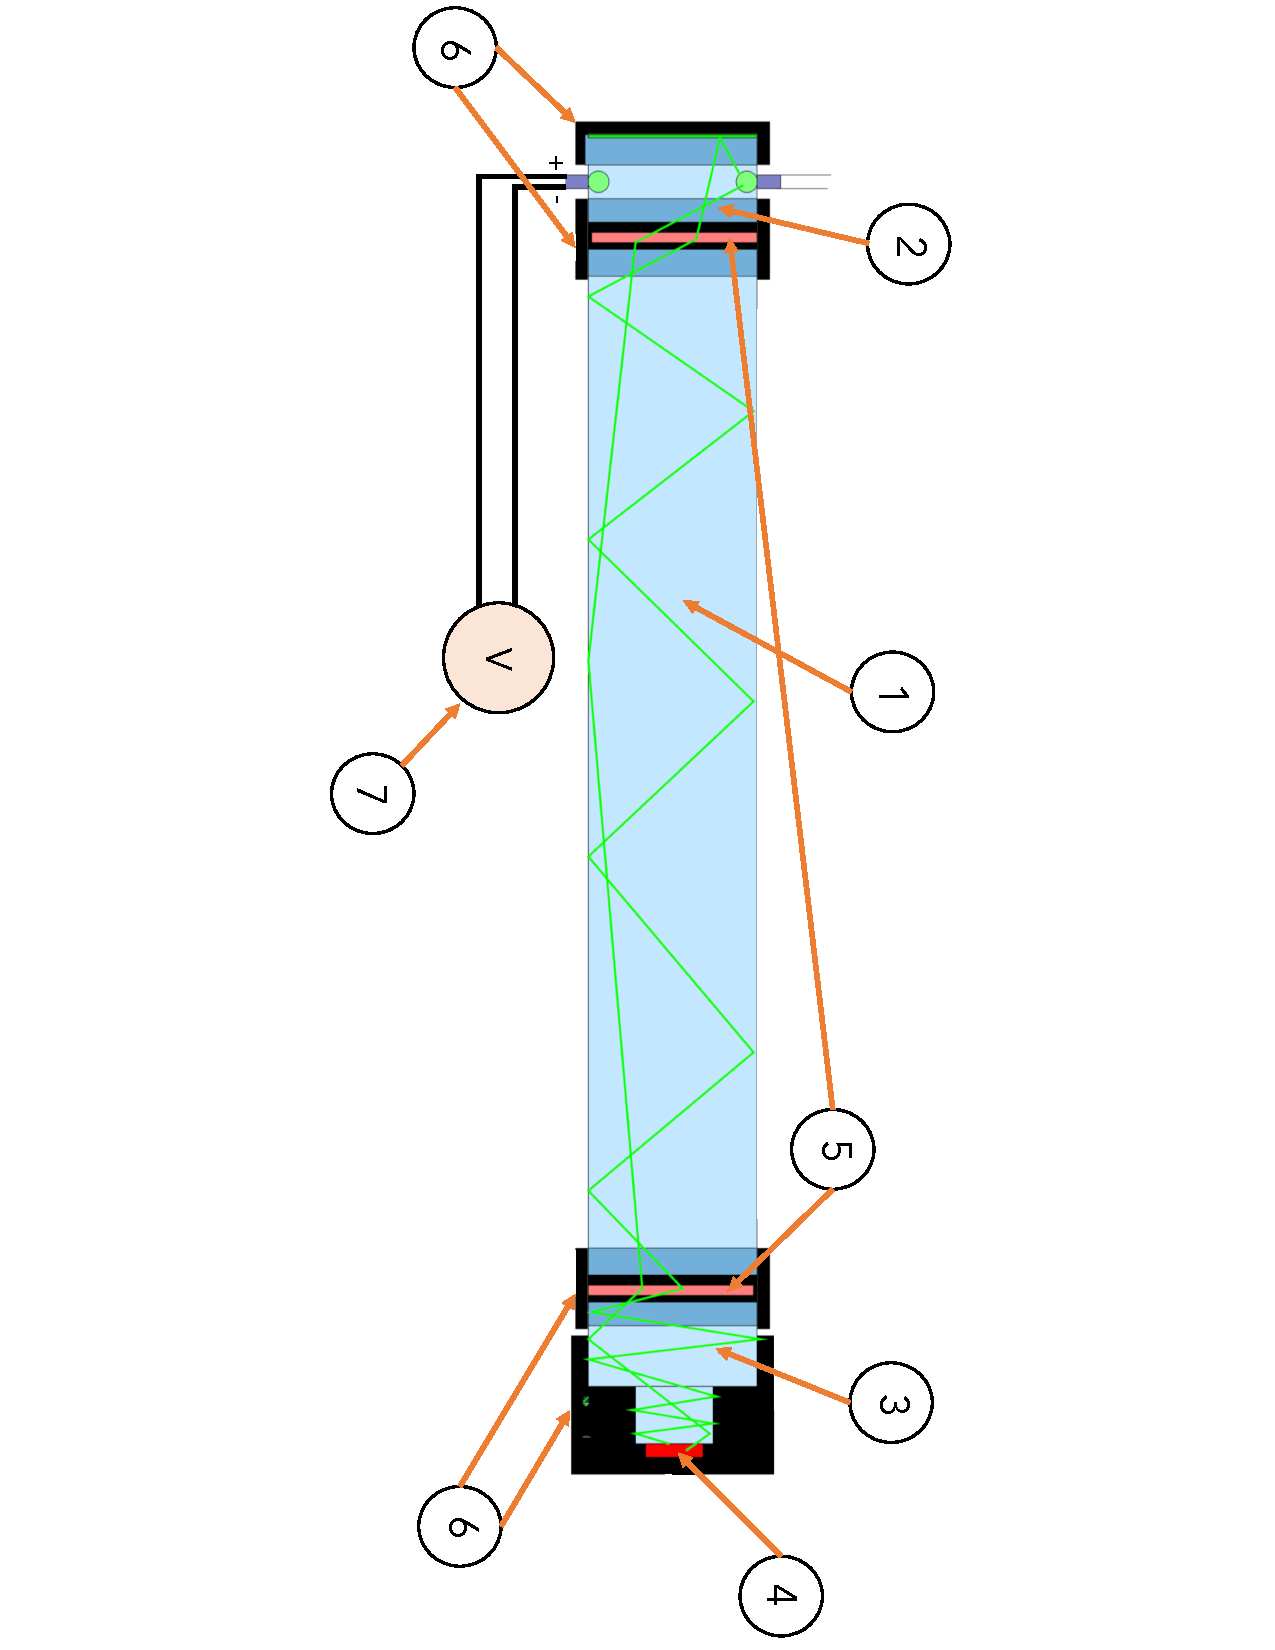
\includegraphics[width=0.35\textwidth,natwidth=610,natheight=642,angle=90]{pics/lg-trans-setup.pdf}}}
\end{picture} 
\caption{Setup for the light guide transmittance measurements. (1) Acrylic rod, (2) light source,
(3) acrylic piece, (4) silicon photodetector, (5) Teflon film as a diffuser, (6) mount units, and (7)
radiometer.}
\label{trans-setup}
\end{figure}
%%%%%%%%%%%%%%%%%%%%%%%%%%%%%%%%%%%%%%%%%%%%%%%%%%%%%%%%%

The measured transmittances were in full accord with our transport calculations (see Section~\ref{lg-mc}).
Studies of our test setup indicated that our measurements were accurate to the few percent level. These
values can be compared directly to measurements of the photoelectron statistics using cosmic ray data for
a configuration with a CTOF scintillation bar coupled directly to a PMT to that where the scintillation bar is
coupled to a light guide. Our findings showed that the ratio of photoelectrons was in agreement with our
bench measurements and our Monte Carlo results.

From the transmittance data the practical attenuation length (see Section~\ref{scint-mat} for a discussion
of practical vs. bulk attenuation lengths) of the light guide can be defined as:

\begin{equation}
\label{pracat}
\lambda= \frac{(l_s-l_x)}{\ln(T)},
\end{equation}

\noindent
which assumes an exponential attenuation of light along the light guide. Our measurements gave
$\lambda$ = 2.3$\pm$0.2~m.

\subsection{Photomultiplier Tube/Voltage Divider Assemblies} 
\label{PMTs}

The selection of the PMTs for the CTOF detector considered a number of different solutions, including
both conventional and field-resistant PMTs. Our final choice, which was thought to be the most conservative
design, opted for conventional PMTs contained within a magnetic shield system at the ends of long light
guides that positioned the PMTs well outside of the high field region of the solenoid magnet.

%%%%%%%%%%%%%%%%%%%%%%%%%%%%%%%%%%%%%%%%%%%%%%%%%%%%%%%%%
\begin{figure}[htbp]
\vspace{5.0cm}
\begin{picture}(50,50) 
\put(-20,200)
{\hbox{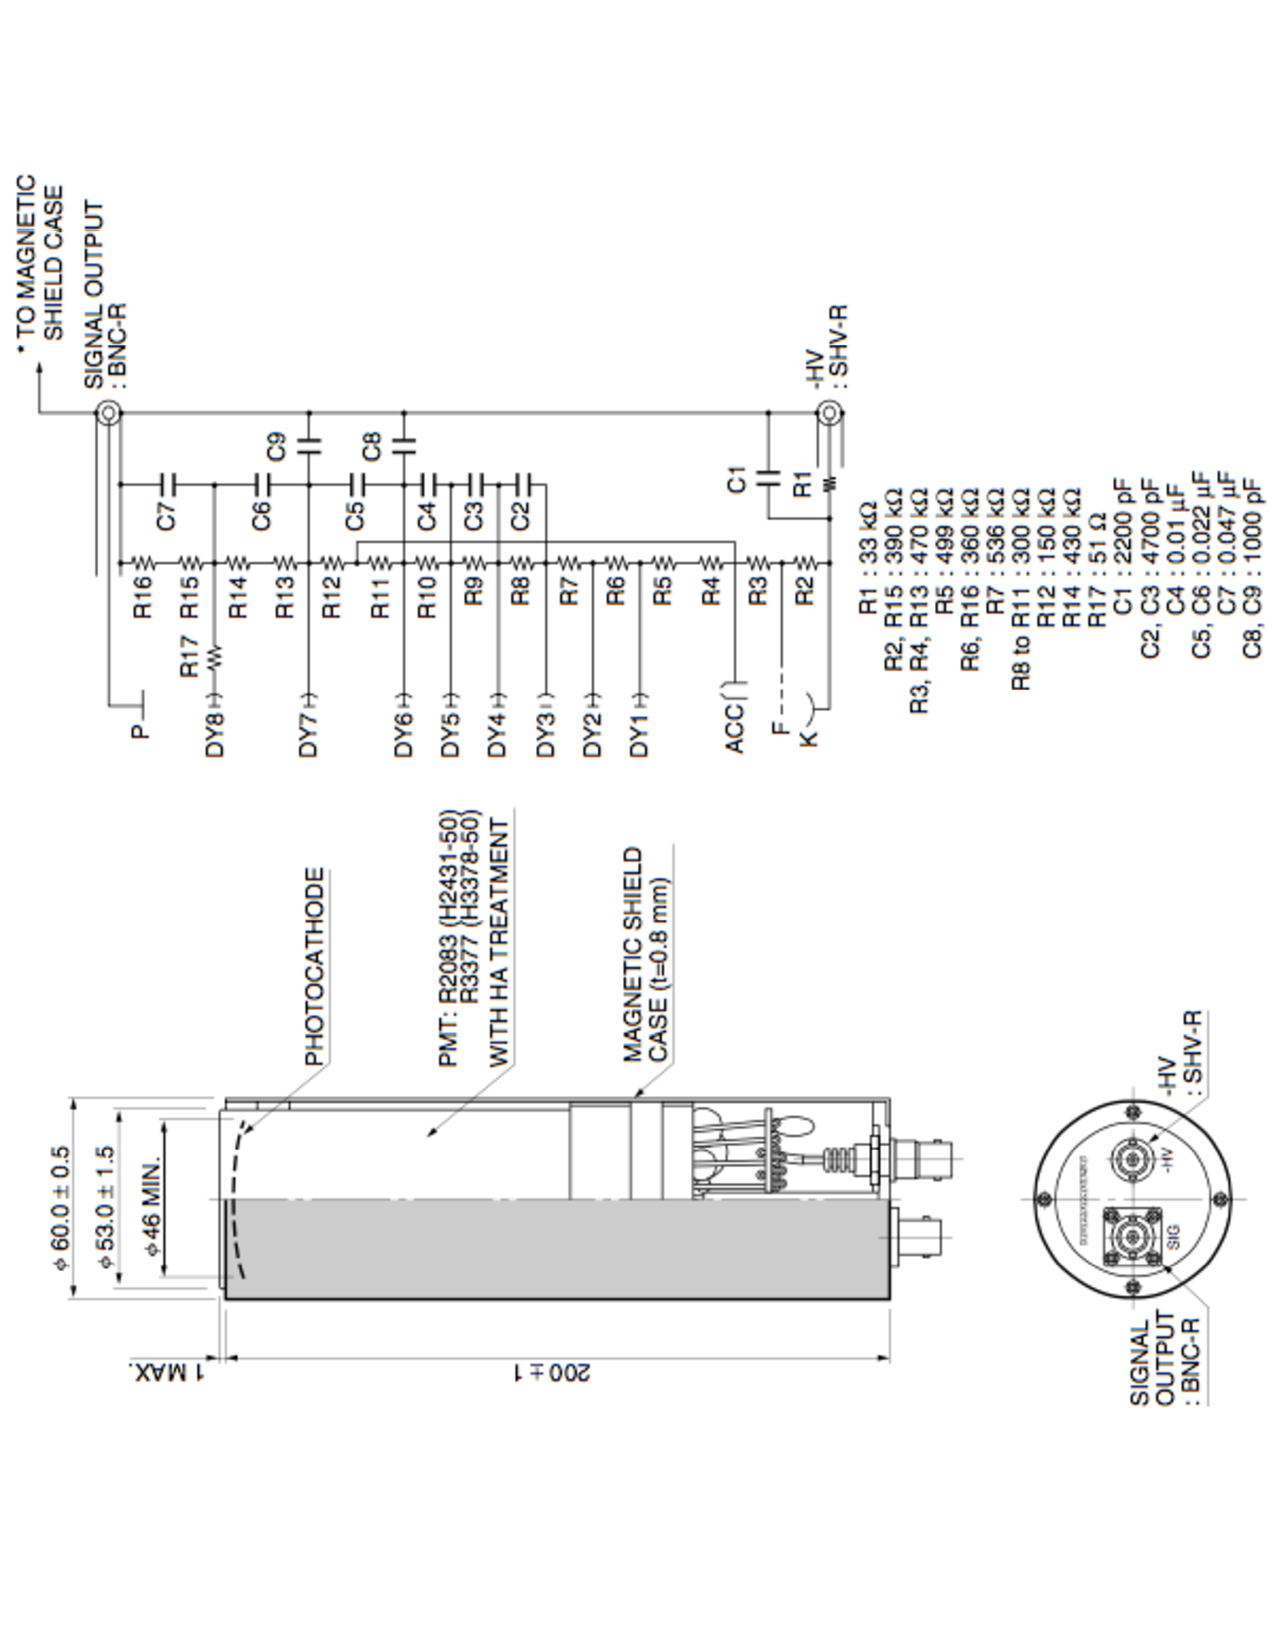
\includegraphics[angle=-90,width=0.47\textwidth,natwidth=610,natheight=642]{pics/h2431.pdf}}}
\end{picture} 
\caption{Schematic diagram of the Hamamatsu H2431 assembly based on the R2083 5.08-cm diameter
PMT used for the CTOF readout~\cite{ham-schem}. Note that for this application the supplied magnetic
shield case was not used.}
\label{H2431}
\end{figure}
%%%%%%%%%%%%%%%%%%%%%%%%%%%%%%%%%%%%%%%%%%%%%%%%%%%%%%%%%

Our choice for the CTOF readout was the H2431 PMT/voltage divider assembly from Hamamatsu. This
integrated assembly employs the 5.08-cm diameter Hamamatsu R2083 PMT. The relevant specifications
for this PMT are listed in Table~\ref{pmt-specs}. Figure~\ref{H2431} shows a schematic of the H2431
assembly and the circuit diagram for the voltage divider. The expectation for these PMTs is that they can
operate in an environment such that the maximum allowable axial field at the photocathode is 0.4~G.
However, we have aimed to achieve fields of $\le$0.2~G at the photocathode to maintain a reasonable
safety margin.

%%%%%%%%%%%%%%%%%%%%%%%%%%%%%%%%%%%%%%%%%%%%%%%%%%%%%%%%%
\begin{table*}[htbp]
\begin{center}
\begin{tabular}{l|l} \hline
Spectral response           & 300 $\to$ 650~nm \\
Wavelength of max. emission & 420~nm \\
Photocathode material       & Bialkali \\
Minimum effective area      & 46~mm \\
Window material             & Borosilicate glass \\
Dynode                      & 8 stage, linear focused \\
Gain                        & 2.5$\times$10$^6$ \\
Quantum Efficiency @ $\lambda_{max}$ & 27\% \\
Max. anode current rating   & 200~$\mu$A \\
Anode dark current (typical) & 100~nA \\
Anode pulse rise time       & 0.7 ns \\
Electron transit time       & 16 ns \\
Transition time spread      & 0.37 ns \\ \hline
\end{tabular}
\end{center}
\caption{The properties of the Hamamatsu R2083 PMT used for the CTOF readout~\cite{r2083-ref}.}
\label{pmt-specs}
\end{table*}
%%%%%%%%%%%%%%%%%%%%%%%%%%%%%%%%%%%%%%%%%%%%%%%%%%%%%%%%%

%%%%%%%%%%%%%%%%%%%%%%%%%%%%%%%%%%%%%%%%%%%%%%%%%%%%%%%%%
\begin{figure}[htbp]
\vspace{0.7cm}
\begin{picture}(50,50) 
\put(-13,-102)
{\hbox{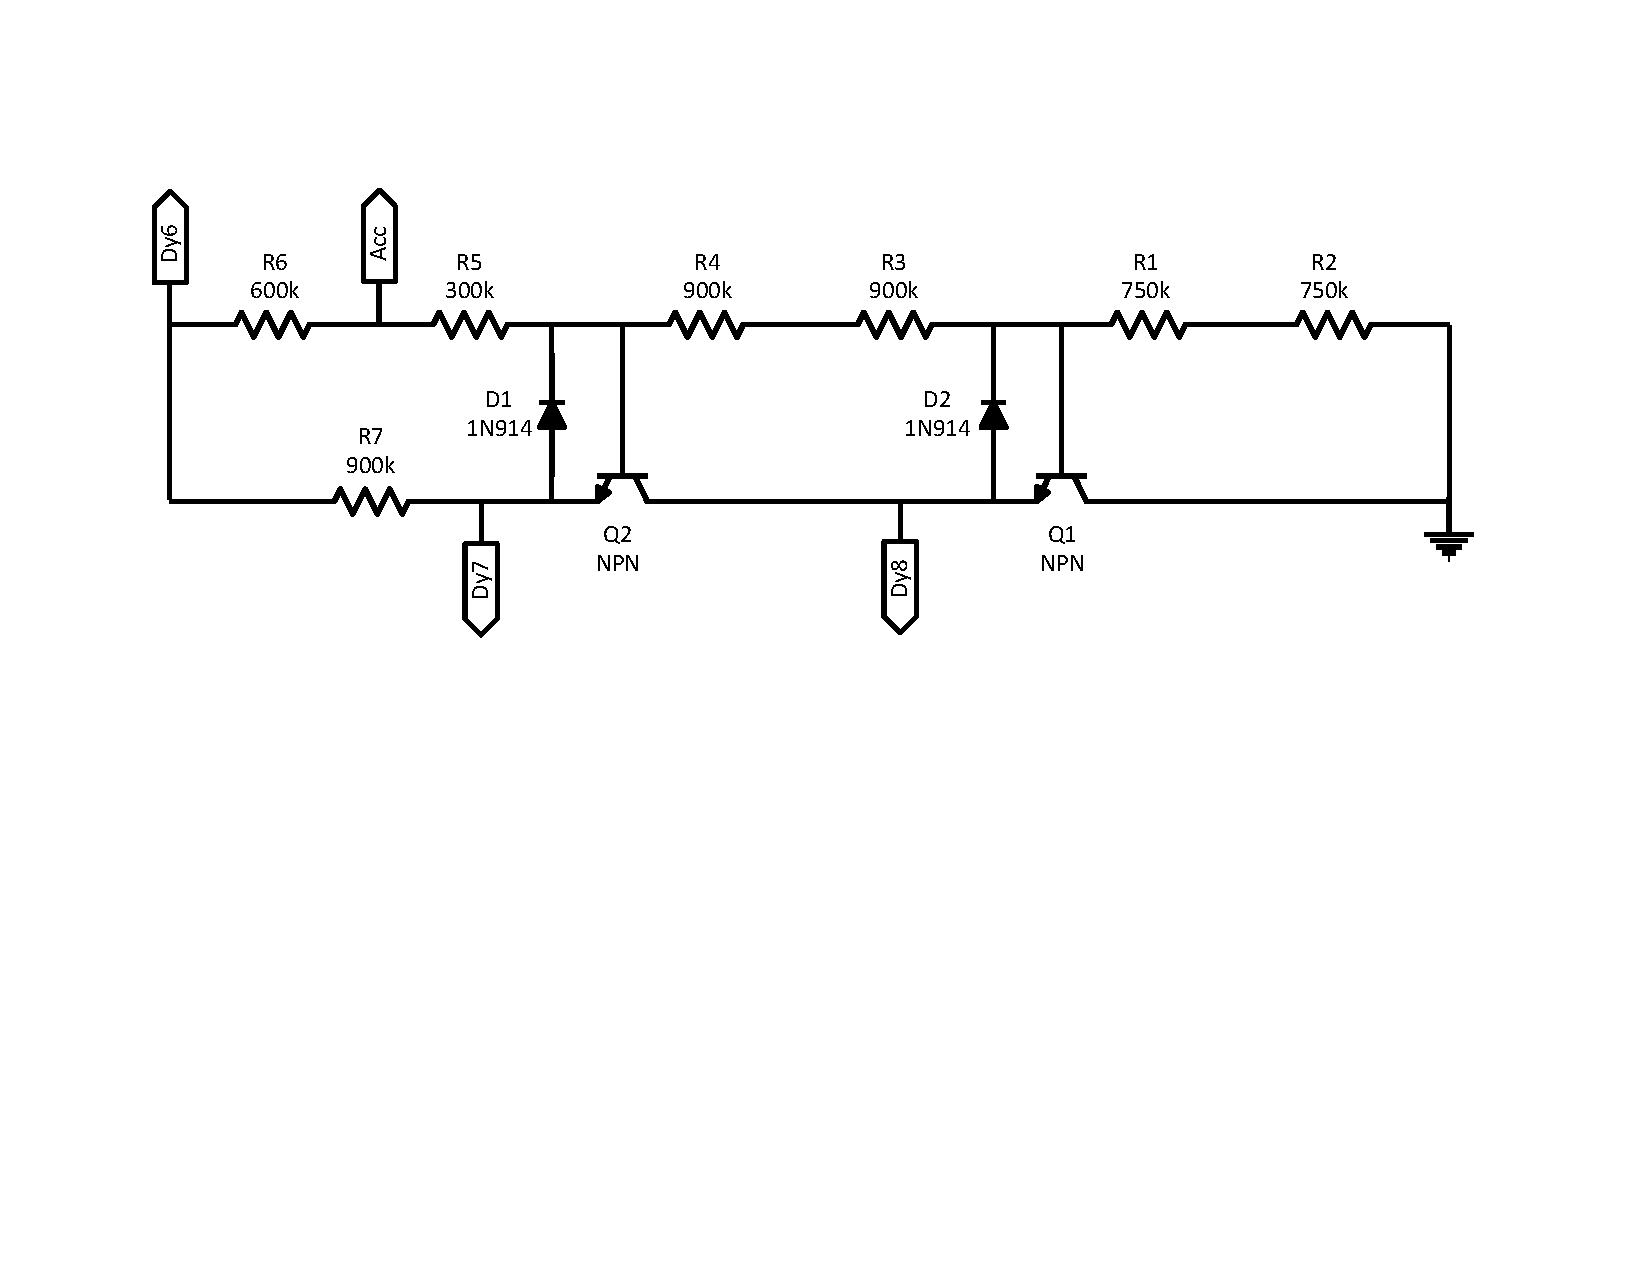
\includegraphics[width=0.42\textwidth,natwidth=610,natheight=642]{pics/amp-circuit.pdf}}}
\end{picture} 
\caption{Schematic diagram of the JLab-designed transistorized impedance matching amplifier 
circuit added to the standard Hamamatsu R2083 voltage divider.}
\label{popov-mod}
\end{figure}
%%%%%%%%%%%%%%%%%%%%%%%%%%%%%%%%%%%%%%%%%%%%%%%%%%%%%%%%%

\subsubsection{Rate-Stabilized Divider}
\label{divider}

The voltage divider circuit shown in Fig.~\ref{H2431} is a standard inclusion with the R2083 PMT in the
Hamamatsu H2431 assembly. Due to the requirement of stable PMT performance in terms of gain and
timing response in the high rate environment of the CTOF detector just outside of the beam-target
interaction region, we modified the stock Hamamatsu divider to improve its stability to higher currents.
A small amplifier circuit has been inserted as a sequential component after the last resistor in the divider. 
This active division circuit consists of two transistors that are powered by the current flowing through the
divider. A version of this circuit design is described in Ref.~\cite{popov}. 

%%%%%%%%%%%%%%%%%%%%%%%%%%%%%%%%%%%%%%%%%%%%%%%%%%%%%%%%%
\begin{figure}[htbp]
\vspace{3.9cm}
\begin{picture}(50,50) 
\put(20,-55)
{\hbox{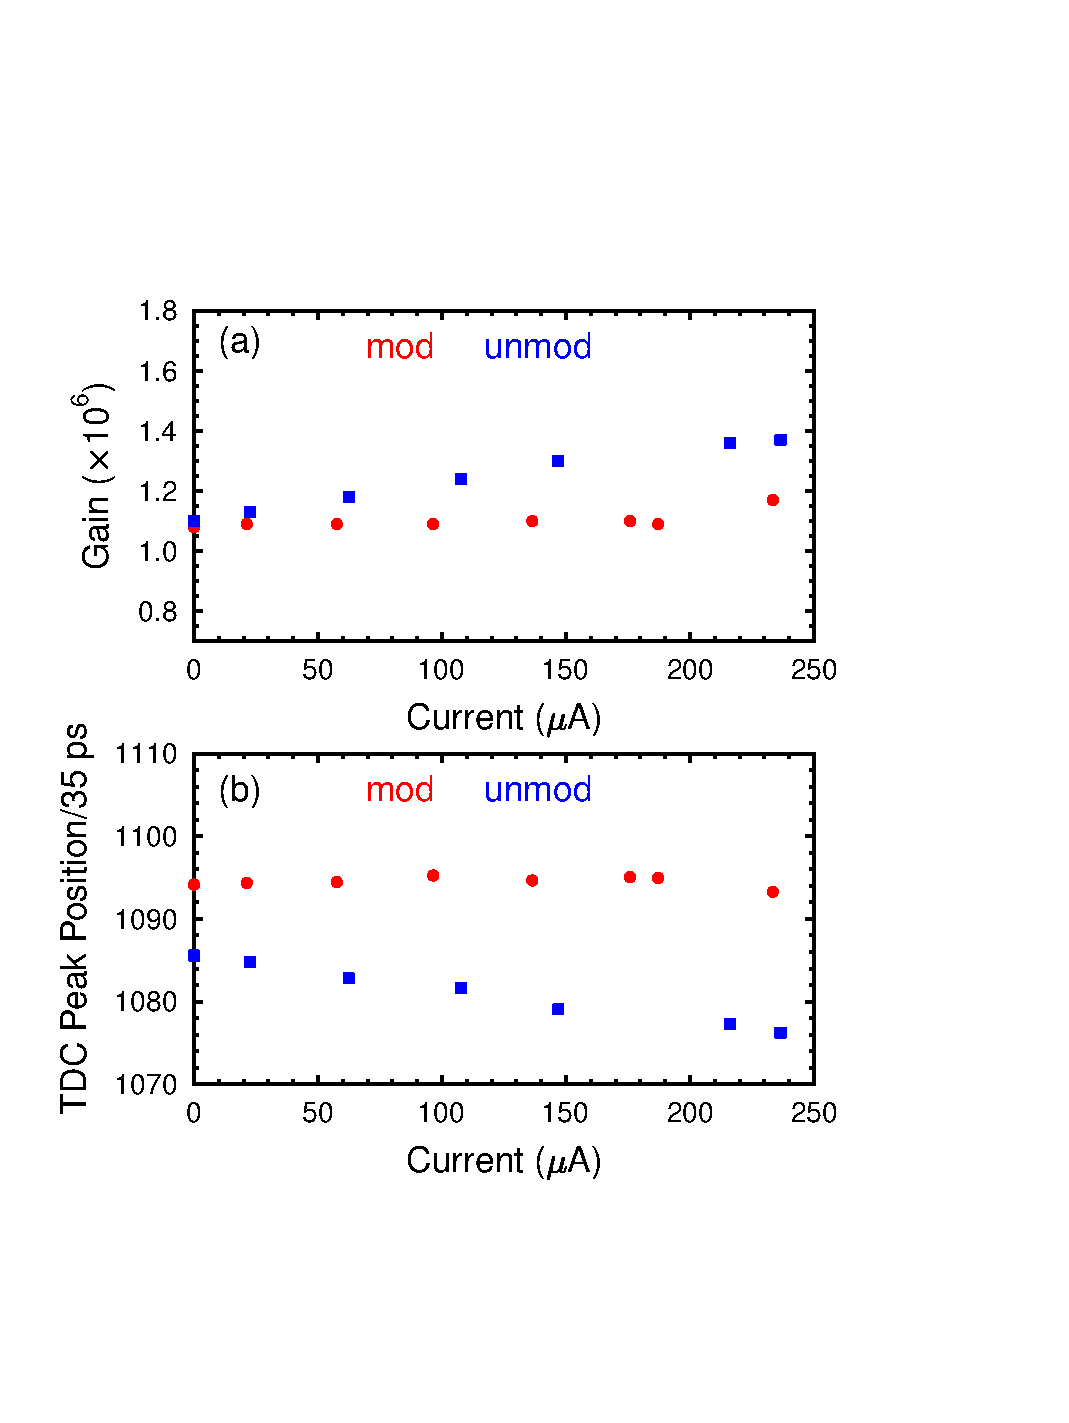
\includegraphics[width=0.52\textwidth,natwidth=610,natheight=642]{pics/divider.pdf}}}
\end{picture} 
\caption{Comparison of the performance of the R2083 PMT vs. PMT anode current ($\mu$A) with its
stock divider (blue squares) compared to that of an R2083 PMT with the modified divider (red circles)
showing (a) the gain stability and (b) the timing response stability.}
\label{mod-div-plots}
\end{figure}
%%%%%%%%%%%%%%%%%%%%%%%%%%%%%%%%%%%%%%%%%%%%%%%%%%%%%%%%%

The active divider amplifier circuit is actually an impedance converter, which provides an output impedance
termination matching to a standard 50~$\Omega$ coaxial cable. The circuit is mounted on a small
mezzanine board that is soldered into the divider. It is connected to Dy6, Dy7, Dy8, ACC (see
Fig.~\ref{H2431}), and grounded as shown in the circuit schematic of Fig.~\ref{popov-mod}. The passive
divider resistors connected to those dynodes were removed and all capacitors were left in place. The 
transistors employed are high voltage (400~V or better rated) Si NPN types. 

Figure~\ref{mod-div-plots} compares the performance of the stock R2083 voltage divider to that of a
typical modified divider. This figure shows a comparison of the gain stability of the PMT/divider
assemblies as a function of the PMT anode current. The gain of the modified divider is seen to be more
independent of current up to 200~$\mu$A, the maximum rated current of the device, compared to the
stock divider. Figure~\ref{mod-div-plots} also shows a corresponding improvement in the stability of the
timing response up to 200~$\mu$A.

\subsection{Magnetic Shields}
\label{sec:shields}

The timing performance of PMTs in external magnetic fields deteriorates due to the Lorentz force. After
an external photon hits the surface of the photocathode and knocks out a primary photoelectron, the electron
accelerates toward the first dynode along the electric field lines. In most timing PMTs, the photocathode is
shaped as a segment of a sphere. The first dynode is located close to the center of this sphere where the
electric field lines concentrate. This design provides for equal travel times for the electrons created at
different parts of the photocathode. However, even an axial magnetic field has a transverse component to
the electric field, and Lorentz forces affect both the propagation time and the destination of the electrons, 
depending on the design of the accelerating electrode. In designing magnetic shields for the CTOF PMTs, we
have been careful to consider both axial and transverse magnetic field components.

To determine the necessary shield reduction factors, the field values at the locations of the PMTs for one
upstream high-pitch angle and one low-pitch angle counter were determined using a map of the CLAS12 solenoid
fringe field based on a full 3-D finite-element analysis (FEA) calculation using the OPERA-TOSCA suite to model
the magnet. Note that due to the azimuthal symmetry of the solenoid fringe field, the field strengths and
gradients at the locations of the full set of upstream high-pitch or low-pitch angle PMTs can be assumed to be
the same. Table~\ref{field-position} provides the field components of the CLAS12 solenoid fringe field at the
locations along the axis of the PMTs at the photocathode (i.e. the face of the PMT), the first dynode (a distance
3~cm from the photocathode), and the middle of the accelerating structure (a distance 5.5~cm from the
photocathode) for both PMTs. All of the fields are necessarily given without any shields present as the shields
strongly modify the local fringe field distributions. Table~\ref{field-position} also includes the field components
along the PMT axes at the locations of the end faces of the shield assemblies. Shield end \#1 is the end closest
to the magnet and shield end \#2 is the end farthest from the magnet. For shield end \#1, the strength of the
field for the high-pitch design is 1000~G and for the low-pitch design is 1076~G. However, due to the different
positions of these shields in the solenoid fringe field, the corresponding axial and transverse field components at
these locations are different.

%%%%%%%%%%%%%%%%%%%%%%%%%%%%%%%%%%%%%%%%%%%%%%%%%%%%%%%%%
\begin{table*}[htbp]
\begin{center}
\begin{tabular} {c|c|c} \hline
               & High-Pitch Angle & Low-Pitch Angle \\ \hline
Position       & $(B_y,B_z)$      & $(B_y,B_z)$  \\
Shield End \#1 & (776, 630) G   & (702, 815) G \\
Photocathode   & (485, 392) G    & (463, 542) G \\
First Dynode   & (390, 313) G     & (444, 209) G \\ 
Middle Dynode  & (318, 265) G   & (303, 361) G \\ 
Shield End \#2 & (261, 227) G   & (245, 308) G \\ \hline
\end{tabular}
\end{center}
\caption{Magnetic field components along the central axis of a representative upstream CTOF PMT of the
high-pitch and low-pitch designs. The magnetic field components are given in a coordinate system with the
$z$-axis along the PMT central axis and the $y$-axis perpendicular to $z$. The associated field components
are from a 3-D field map of the CLAS12 solenoid. The positions are locations along the associated PMT axes
at the photocathode, the first dynode, the middle of the accelerating structure, and at the end faces of the
magnetic shield volumes.}
\label{field-position}
\end{table*}
%%%%%%%%%%%%%%%%%%%%%%%%%%%%%%%%%%%%%%%%%%%%%%%%%%%%%%%%%

For the positioning of the CTOF magnetic shields in the CLAS12 solenoid fringe field, the field lines are at
roughly 40$^\circ$ with respect to the axis of the PMT. In this case roughly two-thirds of the field is axial,
which produces a smaller effect on PMT performance than the transverse component, but is more difficult
to shield. We do not consider here the PMTs at the downstream end of the magnet. However, using the field
map and the known downstream PMT locations, the maximum field strength for the downstream PMTs within
the shield volume is $\sim$400~G. Because we have opted to use an identical shield for all CTOF PMTs, the
discussion here focuses only on the shield design for the upstream PMTs. A shield designed for the fields
seen at the upstream PMT locations will necessarily work to shield the lower field seen at the downstream
PMT locations.

Various multi-layer shield designs for the CTOF PMTs were studied that were comprised of different
coaxial ferromagnetic cylinders. Ultimately we found that a 28-cm-long, three-layer shield composed of 1008
steel of maximum thickness of 1.7~cm for the outer layer, a 3-mm-thick layer of the ferromagnetic alloy
HiPerm-49 (48\% Ni, 0.5\% Mg, 0.35\% Si, 0.02\% C, balance Fe) for the middle layer, and a 0.8-mm-thick
layer of the ferromagnetic alloy Co-NETIC (80.6\% Ni and 14\% Fe) for the inner layer, provided the best
performance within the CTOF magnetic field environment. Modeling calculations and measurements with
physical prototypes showed that such a shield design can reduce a 1~kG external axial field to the level of 
$<$0.5~G at the location of the PMT. To reduce the remaining remnant field to the level of $<$0.2~G, a
compensation solenoid coil is included just outside of the inner ferromagnetic layer. The design of the magnetic
shield system for the CTOF PMTs is discussed in Refs.~\cite{baturin12,cn2015-003}.

In order to make the magnetization more uniform across the outer shielding cylinder, an improved design has
been realized by using a tapered cylinder 1.0~cm thick at the ends and 1.7~cm thick in the middle.  Since both
the magnetic field flux and the material thickness increase linearly toward the middle of the cylinder, the
magnetic field density in the shield layer is almost constant. This maximizes the permeability and results in
significantly lower and more uniform fields inside the cylinder, which improves the shielding capability of the 
inner layers.

Figure~\ref{bshield-3d} shows a cut view of the CTOF PMT shield system from our 3-D design model to
highlight the components that make up the different layers and their positioning with respect to each other. The
inner shield layers are attached to the light guide using a supporting clamp and the steel shield layer is attached
to a support structure secured to the CLAS12 solenoid. Note that both the external and the intermediate shield
layers actually consist of a cylindrical section with conical endcaps that fit tightly together. The conical endcaps
help to capture more field lines at low radial coordinates compared to a flat cylinder. This feature results in a
lower inner field with better uniformity along the central axis. The PMT itself fits within the inner shield cylinder
and the light guide feeds into the opening on the downstream end of the shield. The full weight of each shield
assembly is $\sim$18~kg.

%%%%%%%%%%%%%%%%%%%%%%%%%%%%%%%%%%%%%%%%%%%%%%%%%%%%%%%%%
\begin{figure}[htbp]
\vspace{1.4cm}
\begin{picture}(50,50) 
\put(-30,-66)
{\hbox{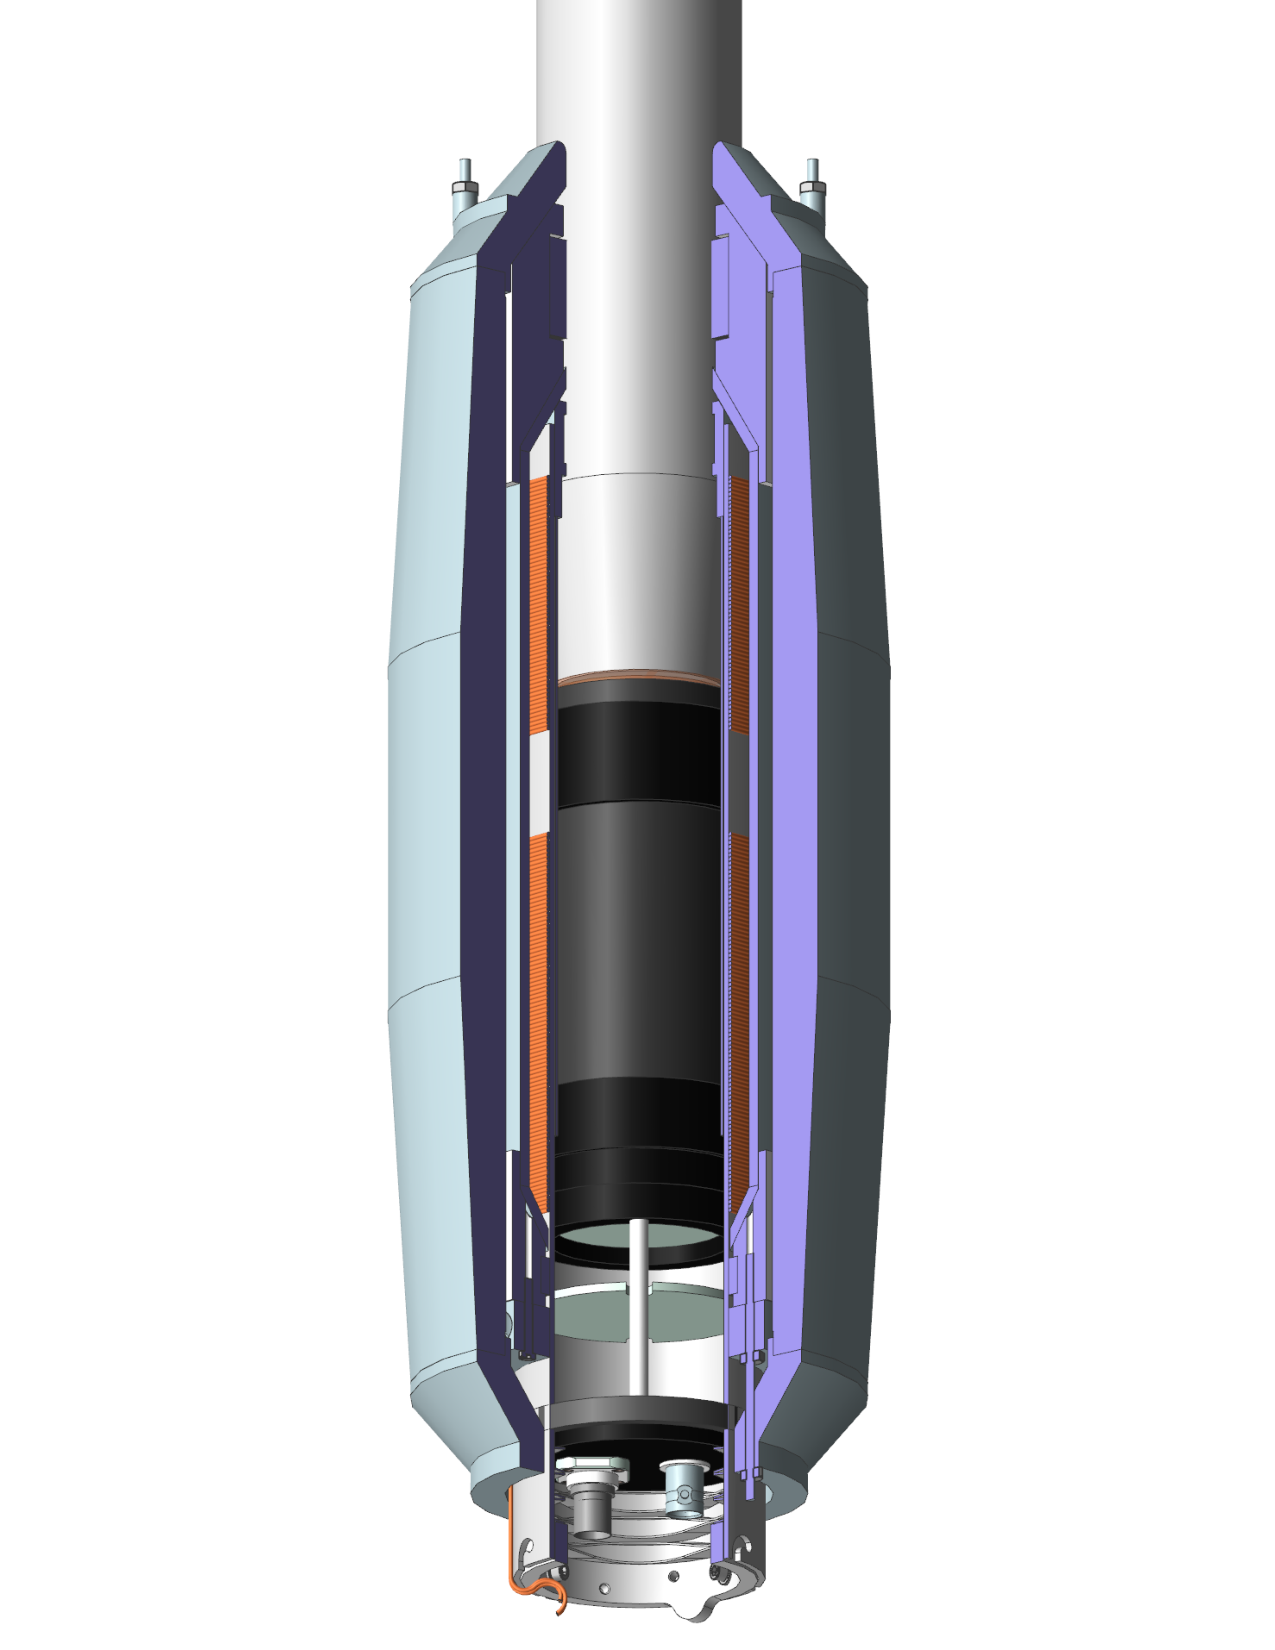
\includegraphics[angle=-90,width=0.53\textwidth,natwidth=610,natheight=642,angle=90]
{pics/bshield.pdf}}}
\end{picture} 
\caption{The CTOF magnetic shield as shown in a 3-D cut view with the different components labeled.
The light guide enters the shield from right side.}
\label{bshield-3d}
\end{figure}
%%%%%%%%%%%%%%%%%%%%%%%%%%%%%%%%%%%%%%%%%%%%%%%%%%%%%%%%%

A compensation coil of 150 turns of 1-mm-thick magnet wire (18~AWG copper with a polyurethane and
polyimide overcoat) was wound on an aluminum mandrel that was positioned between the inner and middle
ferromagnetic layers. The compensation coil consists of two wholly independent coils, the first $z_1$ of
90 turns placed about the middle of the PMT accelerating structure and the second $z_2$ of 60 turns
placed about the PMT photocathode. A gap between the coils was included to achieve a more uniform field
along the PMT axis. 2-D FEA calculations  showed that coil currents on the order of 0.5~A to 1~A were
sufficient to reduce the inner remnant field of 0.5~G to 1~G down to the level of 0.2~G for optimal PMT
response. For these currents, the coils generate a field of 5~G to 10~G at the surface of the mandrel.

It should be emphasized that the compensation coils are placed outside of the innermost ferromagnetic
cylinder. The whole point is that the effective field in the PMT area is a superposition of the ferromagnetic
magnetization, the residual external fields, and the coil field. Unlike the case of an external compensation
coil, the inner coil positioning creates two opposite axial fields. The first field is that of the compensation
coil and the second field with the opposite direction is due to the additional ferromagnetic magnetizations
by the compensation coil. Field calculations were carried out to show that the two opposing fields reduced
the field along the PMT accelerating structure from $\sim$1~G down to $\sim$0.2~G.

For the CTOF shields the compensation coils $z_1$ and $z_2$ are independently controllable. The low
voltage power supply for the coils is a Wiener MPOD mini-crate outfitted with two MPV8016I modules. Each
module has eight channels that can individually provide up to 50~W per channel with a maximum current of
5~A. Each channel powers 12 individual $z_1$ or $z_2$ upstream or downstream coils in series. The coils
corresponding to the upstream low-pitch angle PMTs are on separate channels than for the upstream
high-pitch angle PMTs as the remnant field components inside the shield are slight different. The power
supply is connected to the coils through $15 - 21$~m long power cables. 

In order to optimize the performance of the CTOF magnetic shields, studies were performed using both
2-D and 3-D FEA calculations. Ultimately, full consistency between these approaches was achieved
\cite{cn2015-003}. Full 3-D calculations with the OPERA-TOSCA suite for the CTOF shields in a 1~kG
uniform external field tilted at 40$^\circ$ with respect to the shield axis yielded the results shown in
Fig.~\ref{shield-opera1}, where the field profile is shown as a function of transverse coordinate across the
shield at the location of the photocathode, the first dynode, and the middle of the accelerating structure.
This shows that as the outer shield layer is approached, the field magnitude slightly changes and that the
behavior depends on the coordinate along the axis. Inside the outer ferromagnetic layer, the field magnitude
rises up by a factor of 10 to $>\!10^4$~G due to the very high magnetization of the ferromagnetic material
that may be close to saturation. In the region between the outer and middle ferromagnetic cylinders, the
field magnitude drops by a factor of 10-50 depending on the axial coordinate along the shield. A similar
effect is seen between the middle and the inner layers. At the location of the PMT the field magnitude is
$\sim$0.4~G. Note that the compensation coils were not energized for these calculations. 

%%%%%%%%%%%%%%%%%%%%%%%%%%%%%%%%%%%%%%%%%%%%%%%%%%%%%%%%%
\begin{figure}[htbp]
\vspace{3.0cm}
\begin{picture}(50,50) 
\put(-18,-32)
{\hbox{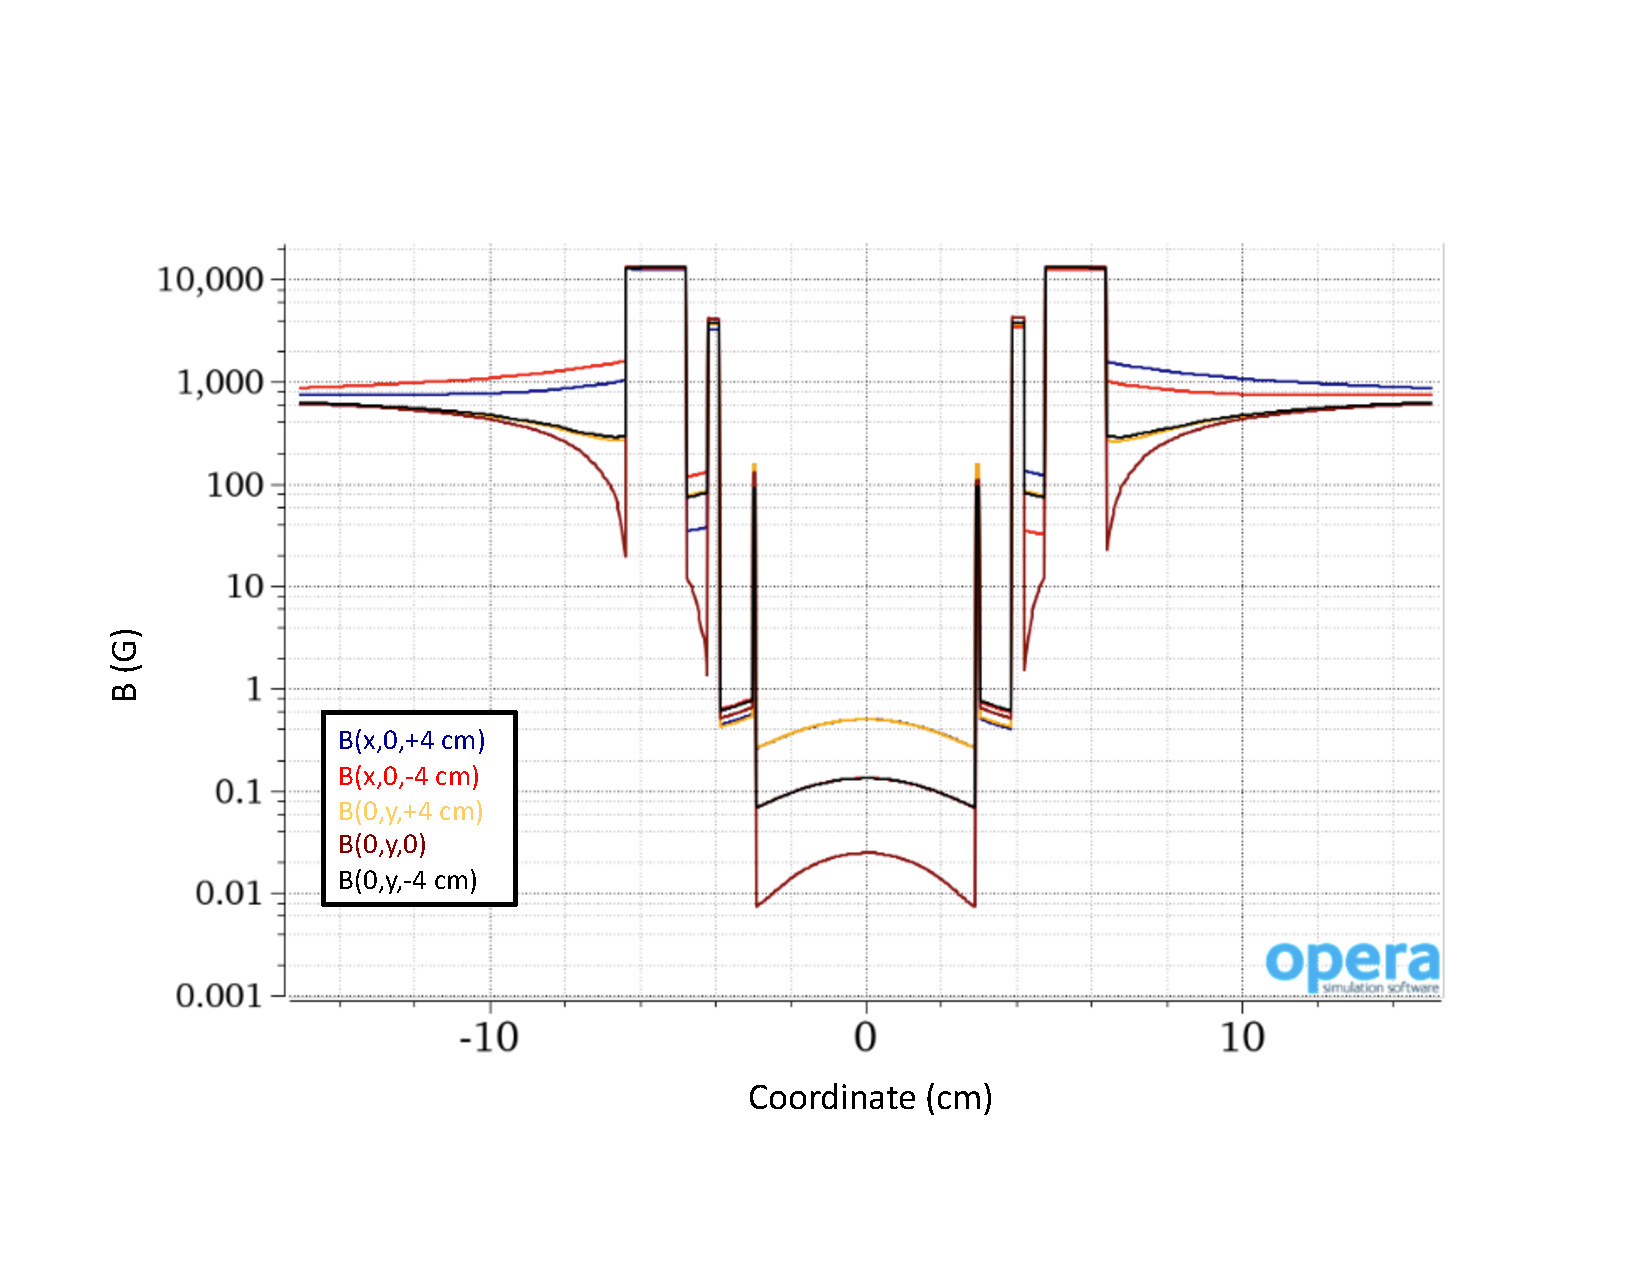
\includegraphics[width=0.44\textwidth,natwidth=610,natheight=642]{pics/opera-mod1a.pdf}}}
\end{picture} 
\caption{3-D FEA Opera calculations for the CTOF PMT shield in a uniform 1~kG field. The field profile
(in G) is plotted across the transverse coordinate (in cm) of the shield. The curves correspond to different
coordinates along the PMT (photocathode at $z$=+4~cm, first dynode at $z$=0, and middle of the
accelerating structure at $z$=-4~cm). The external field lines were at an angle of 40$^\circ$ relative to
the shield to reflect the operational configuration.} 
\label{shield-opera1}
\end{figure}
%%%%%%%%%%%%%%%%%%%%%%%%%%%%%%%%%%%%%%%%%%%%%%%%%%%%%%%%%

In order to validate the 2-D and 3-D FEA calculation results for the CTOF magnetic shield design, studies
were completed placing one of the shields in the fringe field of a 5-T superconducting test magnet. For these
tests the shield was set in the fringe field at positions that matched the field strength and gradient for
what was expected from Table~\ref{field-position} for the shield positioning in the fringe field of the
CLAS12 solenoid. The tests showed that all field components were measured to be less than 0.5~G at all
positions along the PMT volume even with the compensation coils turned off. The studies further showed
that the remnant field could be reduced by a factor of two with the compensation coils set to 1~A (with
$i_{z_1} = i_{z_2}$). The full results from these tests are detailed in Ref.~\cite{shield-test}. The
effectiveness of the shields was also studied after CTOF counter installation in the CLAS12 solenoid. The
PMT gains as seen through the average ADC response for minimum-ionizing particles were in agreement with
the solenoid off and energized to full field.

\subsection{Counter Assembly}
\label{assembly}
           
The counter assembly employed a precision alignment table configurable to match the geometry of the CTOF
counters with both the high-pitch and the low-pitch upstream light guides that was designed to position the
counter component parts into their proper alignment for gluing. To bond the pieces together Bicron BC-600
optical cement was employed. After gluing, the counters were wrapped first in a reflective layer and then
in a fully opaque layer. The reflective wrapping layer employs the Enhanced Specular Reflector VM-2002. This
layer serves to increase the light transmittance along the counter from the charged particle ionization path to
the PMTs. The outer opaque layer employs Tedlar, a polyvinyl fluoride film from DuPont.

The nominal gap between the bare faces of neighboring CTOF scintillation bars in the barrel is 800~$\mu$m.
In order to have sufficient space to form the barrel at its nominal radial position, allowing for assembly and
component tolerances, it was imperative that the wrapping be completed so that there were no wrinkles or
excess material on the inter-counter sides of the bars and that all tape seals were applied only to the inner
and outer radial surfaces of the bars. To meet this requirement both the VM-2002 and Tedlar wrapping
materials were cold-formed using tooling that made precise creases that matched the shape of the scintillation
bars. Full details on the counter wrapping for the scintillation bars are included in Ref.~\cite{ctof-wrapping}.
The final nominal inter-counter gap after wrapping is $\sim$435~$\mu$m.

After wrapping was completed, the counters were secured on storage carts and the magnetic shields were
partially installed. Due to the weight of the shield assemblies, counter testing proceeded without the heavy
steel cylinder and its associated upstream steel cone (see Fig.~\ref{bshield-3d}). These pieces were not
attached to the counters until they were moved to Hall~B for installation into the solenoid using the CTOF
installation strongback that supported the weight of the shields. The installation procedure for the counters
is detailed in Section~\ref{installation}. Full details on the procedures for assembly of the CTOF magnetic
shields are included in Ref.~\cite{ctof-sh-assy}.

With the inner and intermediate shield layers installed on each light guide, the final step of the counter
assembly was to install the R2083 PMTs with their voltage dividers into the shield volume. Note that the
azimuthal orientation of the PMTs within the shield is set to minimize $\vec{v} \times \vec{B}$ effects from
the remnant solenoid field within the shield volume that might otherwise result in loss of photoelectrons from
the acceleration chain. The coupling contact between the PMT and the end of the light guide was made up with
BC-630 silicone optical grease ($n$=1.465) to match the indices of refraction of the two materials. The PMTs
are held against the light guide using pressure from a spring clamp at the end of the voltage divider (see
Fig.~\ref{bshield-3d}).

The storage carts served as the basis for the CTOF cosmic ray test stand and extensive characterizations of
the counters and their performance were completed during the year between the completion of counter
assembly and installation in Hall~B. The results of the cosmic ray studies in the assembly area are detailed in
Section~\ref{sec:performance}.

\subsection{Installation}
\label{installation}

Due to the geometry of the CTOF counters, they were inserted into the solenoid one at a time, with the
insertion taking place from the downstream end of the magnet. For installation each counter was attached
to a stiff aluminum support beam that kept the counter supported along its full length. Using a fixture that
moved along the solenoid axis, the counters were inserted into the solenoid, and rotated into their correct
azimuthal position. The counters are supported by their magnetic shields and brackets that attach along the
upstream and downstream light guides. 

The installation sequence proceeded with installing the counters in quadrants, starting at the bottom position on
the solenoid and installing counters alternating back and forth between the high-pitch and low-pitch designs. The
final counter for insertion (with the low-pitch design) was machined to have a rectangular cross section of 24~mm
width to fit into the last gap in the barrel.

After installation of the counters, survey measurements were taken to ensure counter positioning was within
tolerances and any adjustments necessary were made. The final survey of the counters after installation and
adjustments showed that all counters were positioned radially to within $\pm$3~mm of their design position.
The scintillation bars themselves are stiff enough along their length that they exhibit no appreciable sag
($< 100$~$\mu$m) due to gravitational load. After the counter installation was complete, the signal and
high voltage cables were connected, followed by the power connections to the magnetic shield compensation
coils.

\subsection{Electronics}
\label{sec-elec}

The CTOF counters generate prompt signals for pulse-height and timing analysis. The anode from each PMT
is connected to a passive signal splitter. 20\% of the anode pulse is fed to a JLab-designed flash
analog-to-digital converter (FADC). 80\% of the anode pulse is fed to a constant fraction discriminator (CFD)
connected to a high-resolution time-to-digital converter (TDC). The overall layout of the CTOF electronics
that processes these signals is shown in Fig.~\ref{electronics}.

%%%%%%%%%%%%%%%%%%%%%%%%%%%%%%%%%%%%%%%%%%%%%%%%%%%%%%%%%
\begin{figure}[htbp]
\vspace{3.4cm}
\begin{picture}(50,50) 
\put(0,-20)
{\hbox{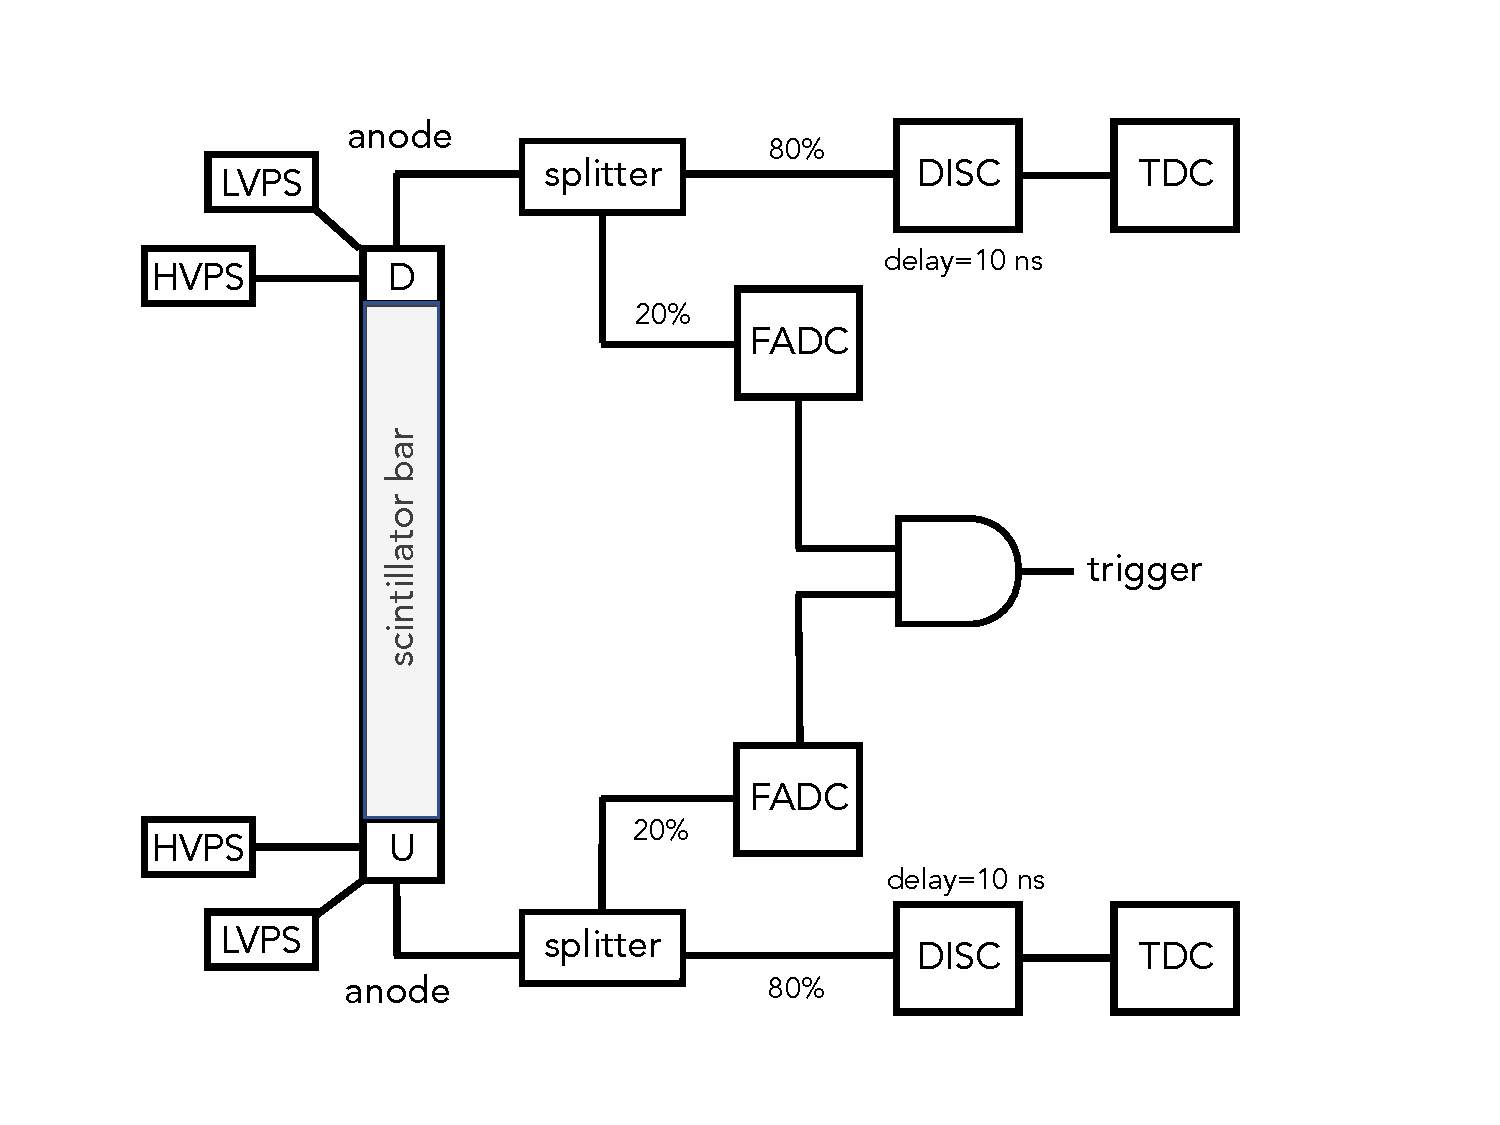
\includegraphics[width=0.43\textwidth,natwidth=610,natheight=642]{pics/ctof-electronics-block.pdf}}}
\end{picture} 
\caption{Block diagram showing the layout of the readout electronics and power connections for a single
CTOF counter.}
\label{electronics}
\end{figure}
%%%%%%%%%%%%%%%%%%%%%%%%%%%%%%%%%%%%%%%%%%%%%%%%%%%%%%%%%

Due to the limited number of channels in the CTOF system, the decision was made to employ CFDs for the
readout. The constant fraction technique permits optimal timing measurements to be made without the need
for sizable offline time-walk corrections to remove the effects of time offsets due to pulses of different
amplitudes crossing threshold at different times. Ortec 935 4-channel 100~MHz CFDs are employed. The
single-width NIM modules accept negative input pulses and generate three simultaneous NIM-standard fast
negative logic pulses for each input pulse that exceeds the set threshold level. The unused bridged outputs
are terminated into 50~$\Omega$ as recommended by the manufacturer.

The constant-fraction shaping delay for each discriminator channel is determined by the length of
external 50~$\Omega$ coaxial cable connected to the channel shaping circuit. To select the optimal
shaping delay the counter time resolutions were studied for delay cables from 4~ns to 16~ns for
each counter relative to a fixed reference time. Figure~\ref{cfd-study}  shows the results of these
studies for a set of 8 counters. The time resolution was seen to improve until a minimum is reached and
then remains relatively flat. Based on these results we chose to use 10~ns delay cables (with the internal
module offset delay omitted) with the time-walk compensation network setup according to the
manufacturer's recommendations.

%%%%%%%%%%%%%%%%%%%%%%%%%%%%%%%%%%%%%%%%%%%%%%%%%%%%%%%%%
\begin{figure}[htbp]
\vspace{2.3cm}
\begin{picture}(50,50) 
\put(25,-135)
{\hbox{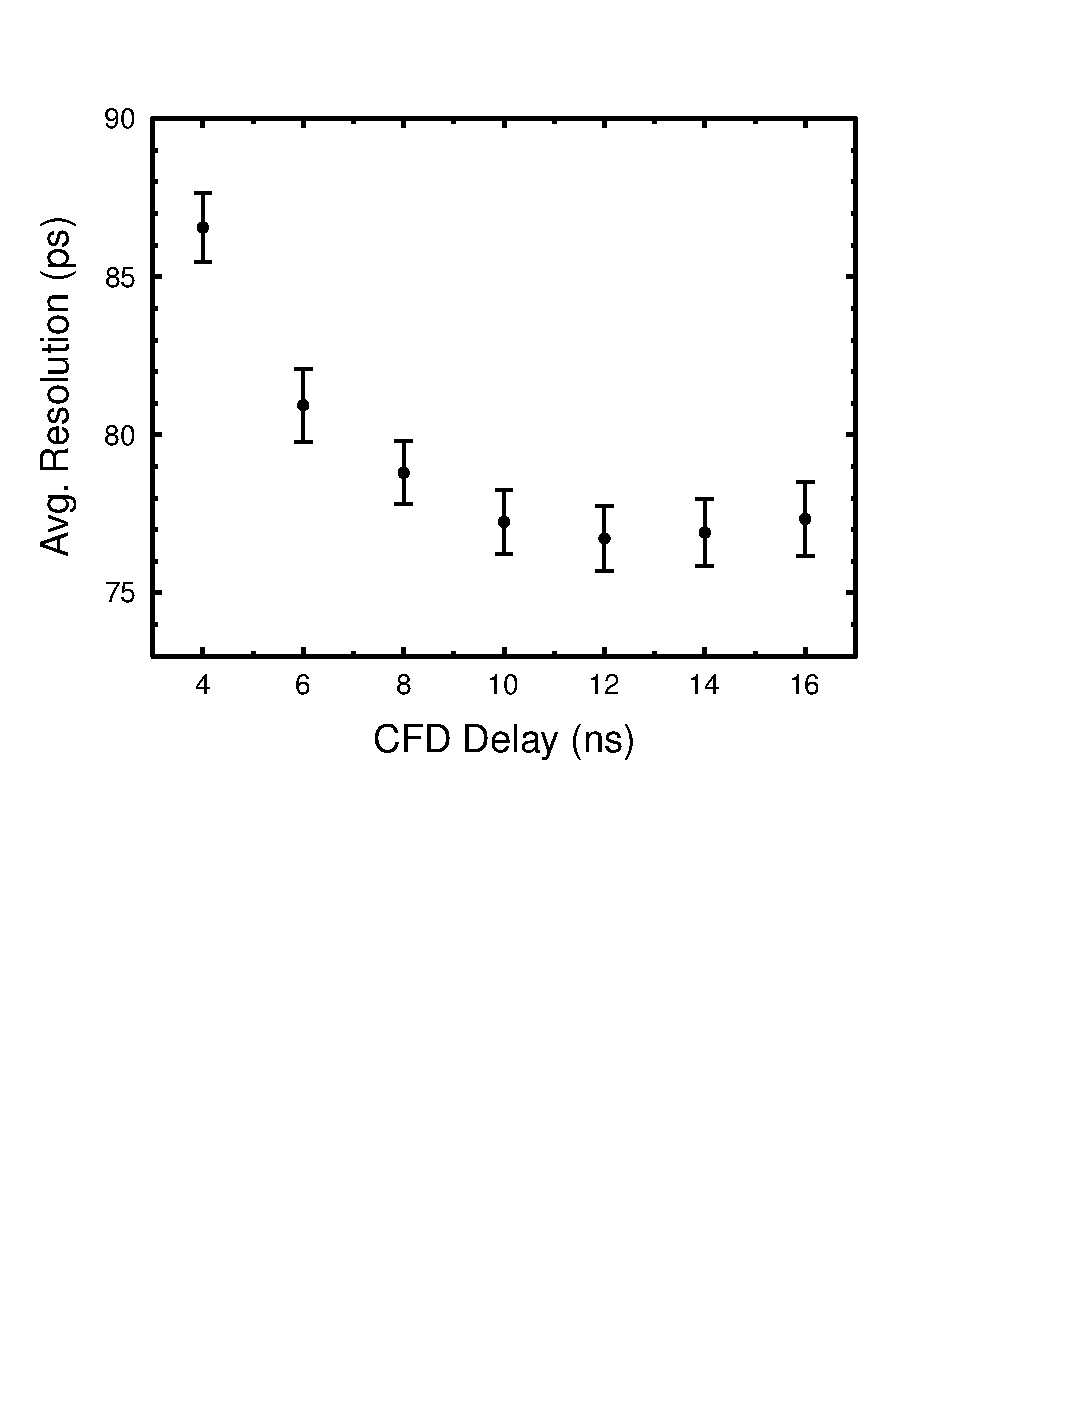
\includegraphics[width=0.52\textwidth,natwidth=610,natheight=642]{pics/res-comp19b.pdf}}}
\end{picture} 
\caption{Average resolution for a set of 8 counters (ps) vs. CFD shaping delay (ns).}
\label{cfd-study}
\end{figure}
%%%%%%%%%%%%%%%%%%%%%%%%%%%%%%%%%%%%%%%%%%%%%%%%%%%%%%%%%

During operation of the CTOF system in Hall~B, the discriminator thresholds were set to 35~mV. After
setting the PMT gains, this corresponded to a threshold of 1~MeV of deposited energy. This threshold is
well below the 6~MeV energy deposited by a perpendicularly incident minimum-ionizing particle.

The output of the discriminator goes to a CAEN VX1290N 16-channel 25~ps LSB (least significant bit)
VME TDC. These multi-hit pipeline TDCs were chosen in order to allow for readout capability at the
operating luminosity of $1 \times 10^{35}$~cm$^{-2}$s$^{-1}$. The TDC readout window was set to 250~ns
to ensure the full dynamic range of the data was safely in time with the trigger. The key performance
specifications of these units are given in Table~\ref{tdcadc-specs}. Note that the integral non-linearity
of each TDC channel in the system was measured and corrected for using a look-up table stored in the
system memory. See Ref.~\cite{daq-nim} for more details.

The PMT signals are also connected to the FADCs for the pulse charge measurement. The readout employs
JLab-designed FADC250 16-channel VME 250~MHz flash ADCs~\cite{fadc-manual}. The key performance
specifications of these units are given in Table~\ref{tdcadc-specs}. Figure~\ref{fadc-pulse} shows a raw
ADC pulse from a representative CTOF PMT where the pedestal has been subtracted. Our procedure
determines the pedestal by averaging over the first part of the readout window before the pulse. This
average is subtracted from the signal region about the ADC pulse. A pulse fitting algorithm that fits the
leading edge of the pulse down to the baseline is used to determine the hit time from the FADC signal and
the charge associated with the pulse. The readout window for the CTOF FADCs is set to 48 samples (192~ns).
The applied readout threshold is set to 1~MeV to ensure that the hit cluster energy can be determined with
a reasonable accuracy. Details on the hit clusterization for CTOF are described in Ref.~\cite{recon-nim}. 

%%%%%%%%%%%%%%%%%%%%%%%%%%%%%%%%%%%%%%%%%%%%%%%%%%%%%%%%%
\begin{figure}[htbp]
\vspace{2.5cm}
\begin{picture}(50,50) 
\put(10,-80)
{\hbox{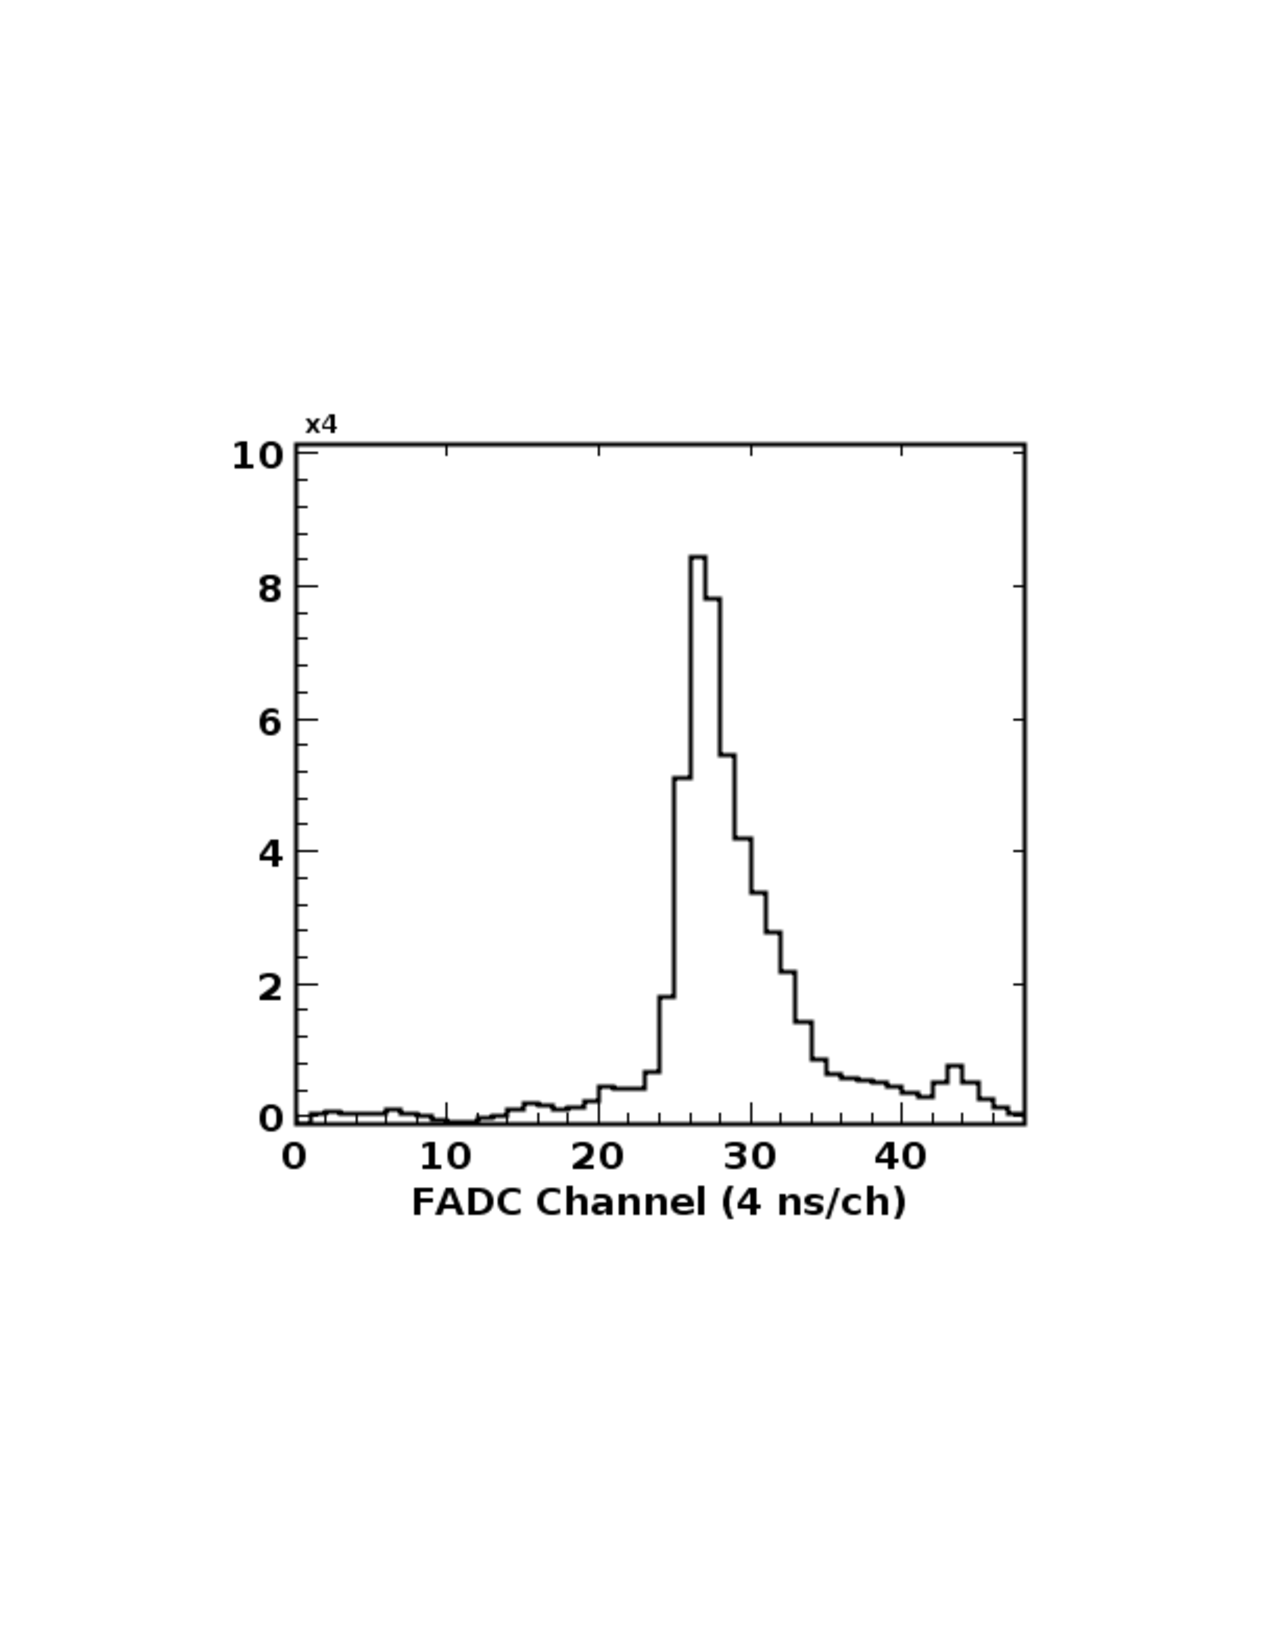
\includegraphics[width=0.45\textwidth,natwidth=610,natheight=642]{pics/ctof-fadc.pdf}}}
\end{picture} 
\caption{Average pedestal-subtracted FADC spectrum from a CTOF counter read out from beam data
with a 10.6~GeV electron beam incident upon a 5~cm liquid-hydrogen target with the JLab FADC250
module.}
\label{fadc-pulse}
\end{figure}
%%%%%%%%%%%%%%%%%%%%%%%%%%%%%%%%%%%%%%%%%%%%%%%%%%%%%%%%%

%%%%%%%%%%%%%%%%%%%%%%%%%%%%%%%%%%%%%%%%%%%%%%%%%%%%%%%%%
\begin{table*}[htbp]
\begin{center}
\begin{tabular}{c|c} \hline
TDC Specs                           & ADC Specs \\ \hline
RMS resolution $\le$ 35~ps          & Sampling 250 MHz \\  
Resolution: 21~bit                  & Resolution: 12-bit \\
Inter-channel isolation $\le$ 3 LSB & Clock jitter 350~fs \\
Double-hit resolution 5~ns          & Data memory 8~$\mu$s \\    
Full-scale range 52~$\mu$s          & Trigger/Data latency 8~$\mu$s / 32~ns \\
\multicolumn{2}{c}{Integral/Differential non-linearity} \\
$<$ 2.5 LSB / $<$ 3 LSB             & $\pm$0.5 LSB / $\pm$0.8 LSB \\
Inter-channel isolation $<$ 3 LSB   & SNR 56.8~dB @ 100~MHz input \\ \hline
\end{tabular}
\end{center}
\caption{The key performance specifications of the CTOF CAEN VX1290N pipeline TDCs and JLab 
FADC250 flash ADCs.}
\label{tdcadc-specs}
\end{table*}
%%%%%%%%%%%%%%%%%%%%%%%%%%%%%%%%%%%%%%%%%%%%%%%%%%%%%%%%%

The PMT anode to splitter panel connections are made using LMR-195 cables, a low-loss variant of RG-58.
LMR-195 is a coaxial cable with a 50~$\Omega$ characteristic impedance. The upstream PMTs were
connected to cable lengths of 15.9~m, 16.3~m, and 16.8~m and the downstream PMTs were connected to
cable lengths of 20.7~m, 21.2~m, and 21.7~m. These cable lengths were required given the location of the
CTOF electronics relative to the PMTs and were made as short as possible to minimize attenuation and
dispersion of the anode signals. The three different cable lengths are connected to neighboring PMTs in
a repeating cyclical pattern to mitigate the effects of possible counter-to-counter cross talk. The signal
connections to the ADCs and TDCs were also set such that neighboring counters were not connected within
the same module. The cable connections from the splitters to the readout electronics used RG-316 cables
of 1.5~m length. RG-316 is a low-loss variant of RG-174 with a 50~$\Omega$ characteristic impedance.

The PMTs for the CTOF counters typically operate at about 1.5-2.0~kV with negative polarity. The typical
dark current drawn by the PMTs on the assembled counters is $<$20~nA. The system is powered by a
single CAEN 527 high voltage mainframe outfitted with negative-polarity 24-channel A1535N modules
that can supply up to 3.5~kV per channel with a maximum current of 3~mA. The power supply has a voltage
ripple specification of $<$20~mV peak-to-peak. Each channel consumes less than 1~W during counter
operation. The typical supply currents per channel are 300~$\mu$A to 500~$\mu$A.

The mainframe is controlled remotely through the Hall~B Slow Controls system. A graphical user interface
using EPICS~\cite{epics} running on a UNIX system communicates with the mainframe via Ethernet. The
mainframe settings enable basic protection of the PMTs in terms of maximum voltage and current settings,
and channel ramp rates.

The high voltage cables for each PMT are fire-retardant RG-59 coaxial cables that run from the voltage
divider to a local disconnect high voltage (HV) distribution box. There are two 48-channel HV distribution
boxes for the CTOF. The output of each HV distribution box is a pair of 35-ft long multi-conductor cables,
each containing 24-channels, with a Radiall connector to mate with the CAEN HV A1535N board input
connector. Each multi-conductor high voltage cable contains individual conductors wrapped in Tefzel
insulation, an outer wire shield, and a PVC insulation wrap, with each conductor rated at 5~kV.

\section{CTOF Performance}
\label{sec:performance}

This section highlights the performance results of the CTOF system from the bench studies, including
the counter photoelectron statistics measurements and the benchmark intrinsic counter time resolutions.
The algorithms employed to calibrate the CTOF and quantify its counter time resolution are also presented.
The effective counter time resolutions with data from the first beam runs for CLAS12 in 2018 are shown.
Finally, this section provides the current status of the particle identification capabilities of the CTOF system.
These results can be compared against the performance specifications as detailed in Table~\ref{spec-table}
to demonstrate the preliminary limits of the charged particle identification for CLAS12 in the central
direction based on the current calibration and reconstruction status.

\subsection{Bench Measurements}
\label{sec:bench}

\subsubsection{Counter Photoelectron Statistics}
\label{sec:npe}

The primary approach to determine the average number of photoelectrons at the photocathode of a PMT
generated by minimum-ionizing particles passing through the scintillation bars employs the ratio of the
integral of the pulse for a minimum-ionizing particle to the integral of a pulse for a single photoelectron.
For these measurements we used a 350~MHz (4 GSa/s) oscilloscope with a pulse averaging mode to average
over 1000 pulses. The minimum-ionizing particle signals were analyzed by connecting the scope to a PMT
mounted on one of the CTOF counters. For the single photoelectron signal, we took data using a bare PMT
on the bench using the same HV setting. For both measurements the oscilloscope threshold was adjusted
appropriately. For the minimum-ionizing peak analysis the threshold had to be set high enough ($>$200~mV)
to eliminate tracks that did not pass fully through the bar. For the single photoelectron peak the threshold
had to be set low enough (1~mV) to pick out the single-electron emission noise pulses from the photocathode
that are the dominant source of the PMT intrinsic dark current. This somewhat crude measurement yielded
200 photoelectrons per MeV of deposited energy at a gain of 1$\times$10$^6$, corresponding to
0.03~nC/MeV.

\subsubsection{Intrinsic Counter Time Resolution}
\label{sec-bench}

The algorithm used on the test bench to determine the time resolution of a given counter was to use cosmic
ray tracks to compare the measured time for each counter to the time measured by two other identical
counters in a triplet configuration (see Fig.~\ref{triplet}). For this measurement, where the track passes
through all three counters with double-sided readout, six times are measured ($t_1 \to t_6$). Each time
measurement represents the difference between the discriminated PMT signal (TDC start) and the trigger
time (TDC stop from the six PMT coincidence). These time measurements are then translated into three
counter hit times $t_{t,m,b} = \frac{1}{2}(t_{1,3,5} + t_{2,4,6})$.

%%%%%%%%%%%%%%%%%%%%%%%%%%%%%%%%%%%%%%%%%%%%%%%%%%%%%%%%%
\begin{figure}[htbp]
\vspace{2.0cm}
\begin{picture}(50,50) 
\put(25,-5)
{\hbox{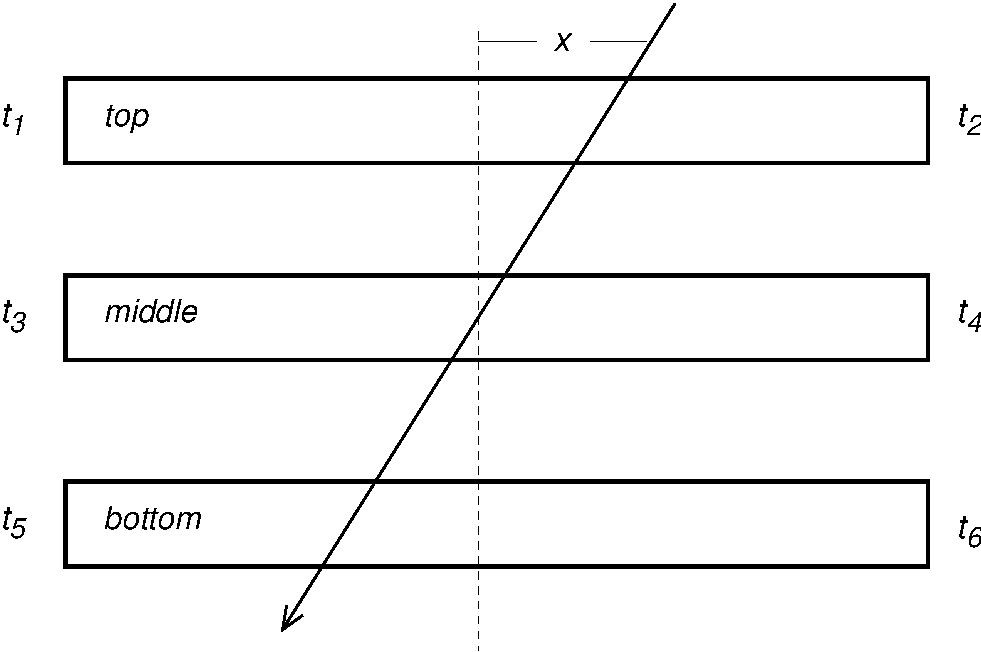
\includegraphics[width=0.47\textwidth,natwidth=610,natheight=642]{pics/triplet-alt.pdf}}}
\end{picture} 
\caption{Schematic representation of a triplet of counters (labeled top - $t$, middle - $m$, bottom -
$b$) with a cosmic ray track traversing the stack. The geometry of the triplet is configured such that
the counters are equally spaced.}
\label{triplet}
\end{figure}
%%%%%%%%%%%%%%%%%%%%%%%%%%%%%%%%%%%%%%%%%%%%%%%%%%%%%%%%%

For incident tracks that pass fully through each counter of the triplet, we can define a time residual
$t_r = t_m - \frac{1}{2}(t_t + t_b)$, where we should expect that the time $t_m$ of the middle scintillator
hit should be the average of the measured times $t_t$ and $t_b$ for the top and bottom scintillator hits,
respectively. Thus the measured residual $t_r$ should nominally be 0. However, due to the smearing of the
measured times $t_t$, $t_m$, and $t_b$ due to the finite time resolution of the measurements, the residual
time $t_r$ will be smeared. The width of the $t_r$ distribution can be used to determine the average time
resolution of each counter in the triplet. For the outer counters in the triplet, the definition of the time
residual must be slightly modified to account for the small path length difference between the reference
counter and the other two counters.

The average time resolution of each counter is computed from the variance $\delta t_r$ in the measured
time residual $t_r$. Assuming the average time resolution for each PMT in the triplet is identical and taking
into account that each counter is readout using two PMTs, we can write the final expression for the average
counter time resolution as:

\begin{equation}
\label{sig-counter}
\sigma_{counter} = \frac{2}{\sqrt{6}} \delta t_r.
\end{equation}

\noindent
Thus a measure of the width ($\sigma$) of the time residual distribution provides a measure of the
average resolution of each counter in the triplet. 

Figure~\ref{res-avg} shows the average time resolution measured for each CTOF counter using the
triplet counter configuration. This analysis included a minimum ADC cut to remove events with low photon
statistics that did not pass through the full width of the counter and also a coordinate cut of $\pm$10~cm
about the center of the scintillation bar. Here the average counter time resolution is 70~ps. The resolution
on average is 15-20\% worse for the top and bottom counters of each cart due to the uncertainties in the
path-length corrections mentioned above. Given the limitations in these measurements discussed below, these
results are quite encouraging compared to the design specifications.

%%%%%%%%%%%%%%%%%%%%%%%%%%%%%%%%%%%%%%%%%%%%%%%%%%%%%%%%%
\begin{figure}[htbp]
\vspace{2.8cm}
\begin{picture}(50,50) 
\put(25,-50)
{\hbox{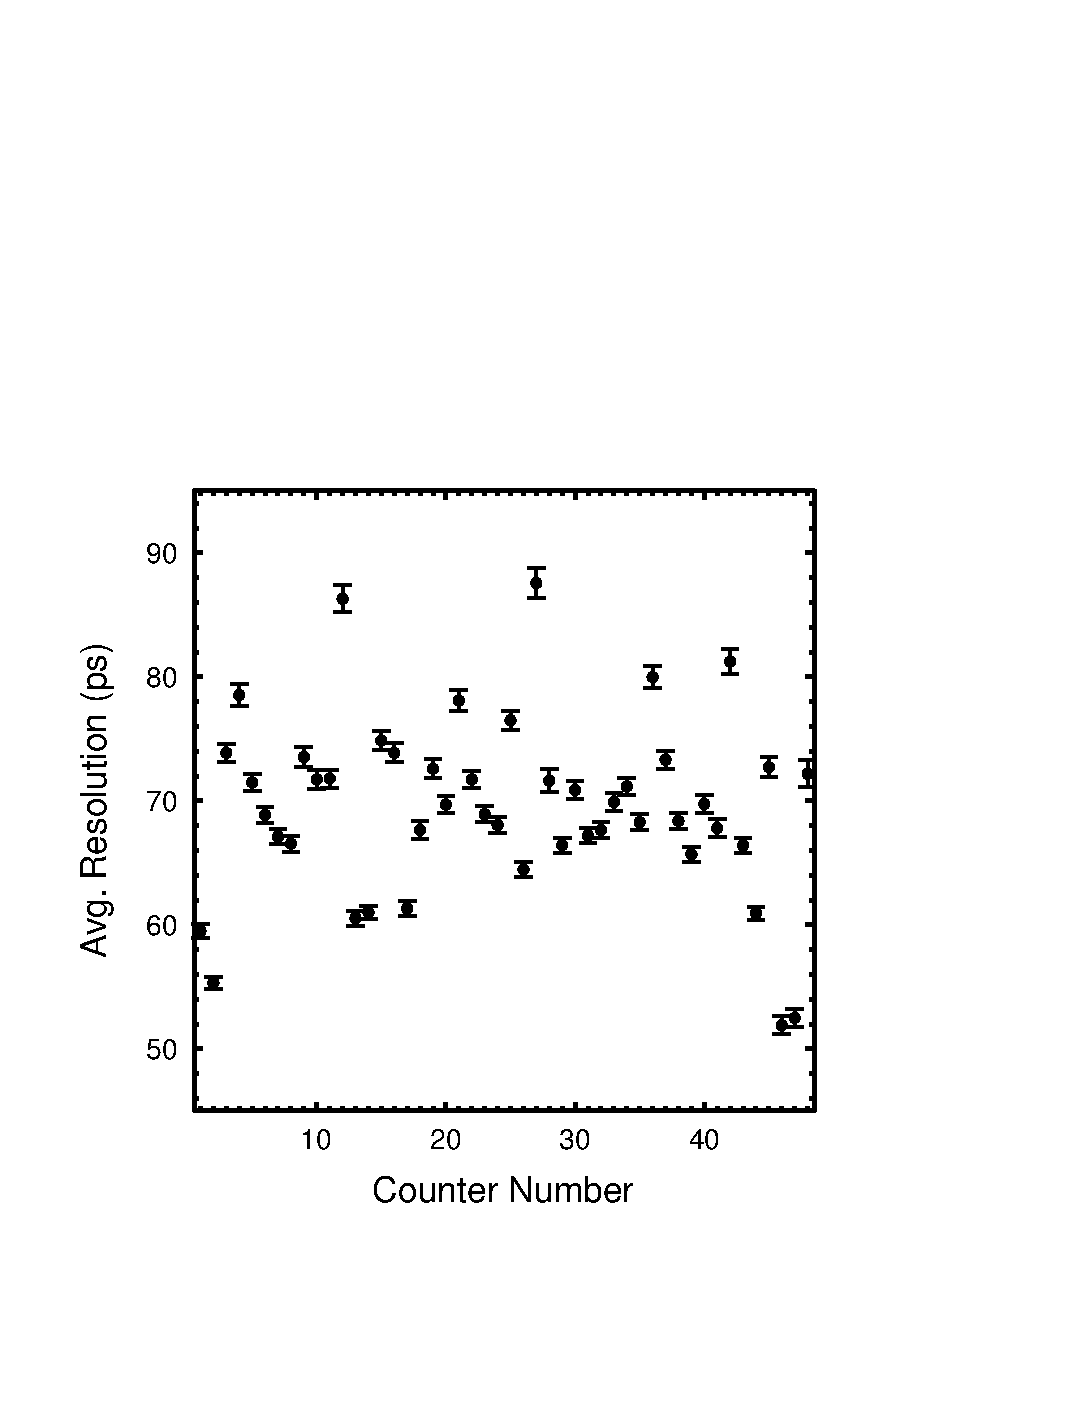
\includegraphics[width=0.50\textwidth,natwidth=610,natheight=642]{pics/res-comp35.pdf}}}
\end{picture} 
\caption{Measured average CTOF counter resolution with cuts on the measured ADC values and the
measured hit coordinates to select events going through the middle of the counter.}
\label{res-avg}
\end{figure}
%%%%%%%%%%%%%%%%%%%%%%%%%%%%%%%%%%%%%%%%%%%%%%%%%%%%%%%%%

Figure~\ref{res-ctof2} shows the average resolution for a representative CTOF counter as a function
of hit coordinate, ADC value, and track incidence angle. The resolution is optimal about the center of
the counter and gets worse near the ends where one PMT receives its minimum light due to attenuation
length effects. The resolution is reasonably flat over the ADC range corresponding to minimum-ionizing
tracks more or less perpendicularly incident upon the counters (channel 2000 for these studies). The
resolution improves with increasing angle due to a correspondingly longer path through the scintillation
material that results in increased photo-statistics.

%%%%%%%%%%%%%%%%%%%%%%%%%%%%%%%%%%%%%%%%%%%%%%%%%%%%%%%%%
\begin{figure}[htbp]
\vspace{1.3cm}
\begin{picture}(50,50) 
\put(-3,-128)
{\hbox{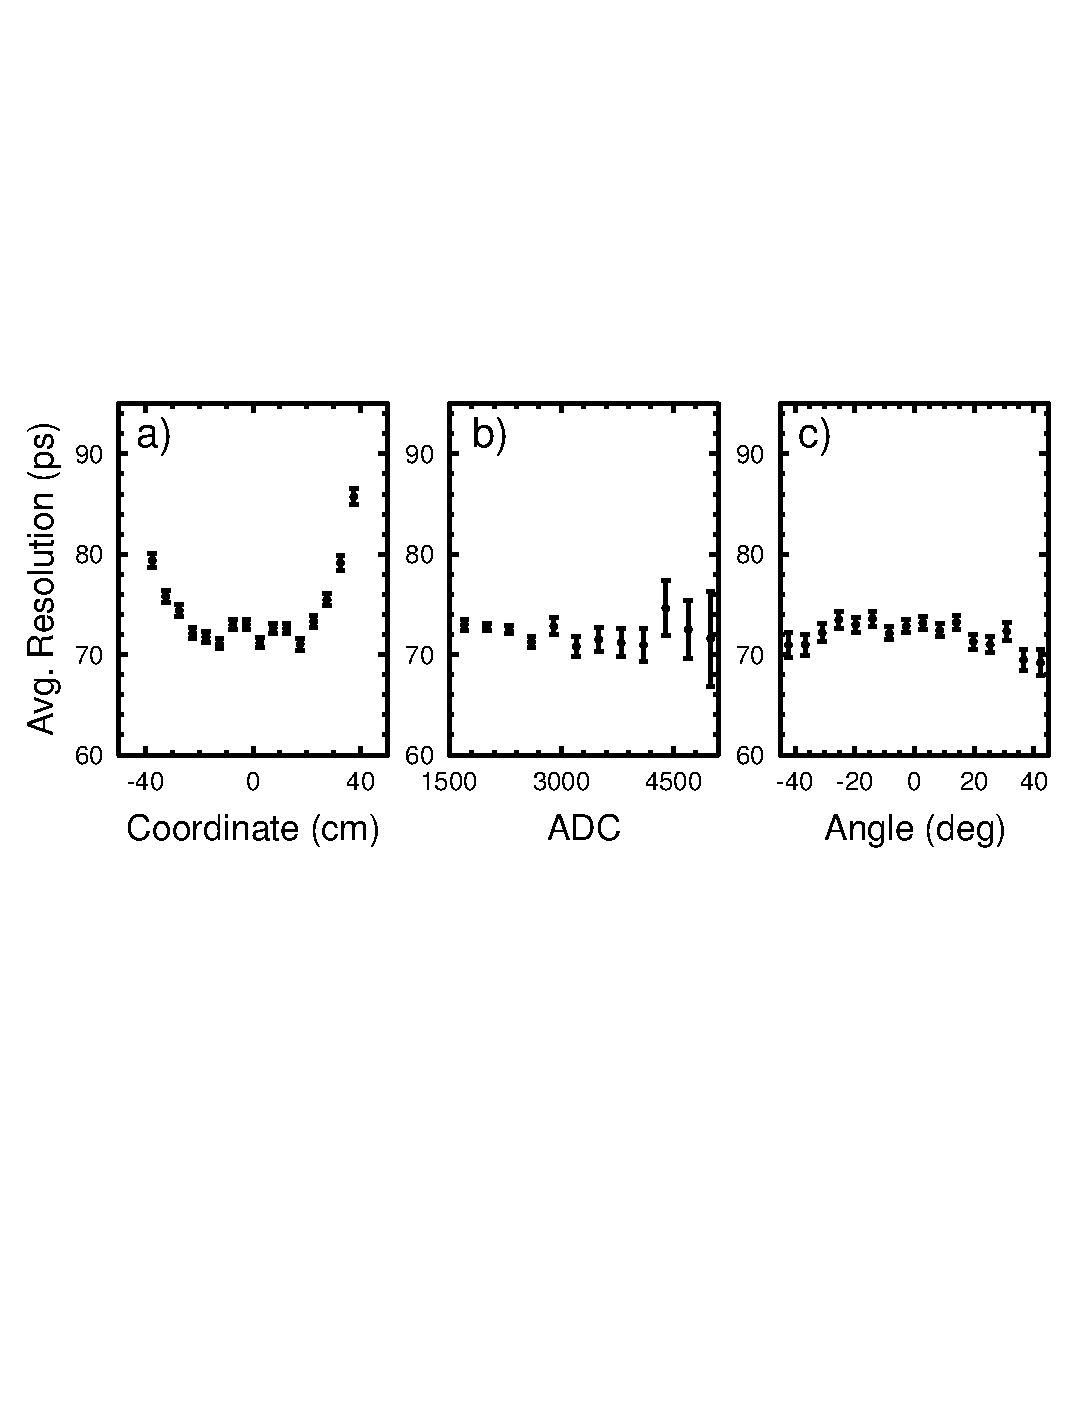
\includegraphics[width=0.57\textwidth,natwidth=610,natheight=642]{pics/res-dep.pdf}}}
\end{picture} 
\caption{Dependence of the counter time resolution for a representative counter on a) the coordinate of
the reference counter, b) the average reference counter ADC value, and c) the angle of incidence of the
track.}
\label{res-ctof2}
\end{figure}
%%%%%%%%%%%%%%%%%%%%%%%%%%%%%%%%%%%%%%%%%%%%%%%%%%%%%%%%%

There are two factors involved in the bench test studies that limited the accuracy of the measured
counter time resolutions. The first arose from the extremely low data rate for each triplet of counters
($< 0.1$~Hz) due to the narrow counter width and the average counter-to-counter separation of
$\sim$22~cm. Data runs of $\sim$1~week were necessary to collect sufficient statistics to determine
the counter resolutions. The inherent calibration drifts over this time could not be tracked precisely. The
second factor arose due to the counter-to-counter alignment within the carts, which  was only at the level
of $\pm$0.64~cm due to the fairly crude design of the carts and the counter supports, which were mainly
intended for counter assembly, wrapping, and storage. The inaccuracies of the alignment were such that the
residual centroids were correlated with the hit coordinates. The contributions of both factors smeared the
measured time resolutions by up to 15\%.  Further details on the bench test performance results for CTOF
are provided in Ref.~\cite{dsc-cn2016-009}. 

\subsection{Beam-Data Calibrations}

In the nominal data taking mode for CLAS12, whenever the CTOF is involved in an event that triggers
the spectrometer readout, the ADCs and TDCs for all PMTs with a signal above the readout threshold
are recorded. For the FADCs, the charge of the pulse is integrated over the extent of the pulse region
and the pedestal is subtracted event by event during offline data processing. For the TDCs the time
recorded is relative to the trigger. To determine the flight time of the charged track from the target to
the CTOF, the TDC time must be correlated with the time of the accelerator radio frequency (RF) pulse.
The RF signal from the accelerator has a period of 2.004~ns. The RF bunch length itself corresponds to
about 2~ps. Although the timing signal is very accurate (with a resolution of $<$20~ps), the determination
of which beam bunch produced a given interaction must be determined by the experiment. Note that for
the initial beam operations with CLAS12 the electron beam was actually delivered in every other beam bunch,
resulting in an effective $T_{RF}$ of 4.008~ns.

%%%%%%%%%%%%%%%%%%%%%%%%%%%%%%%%%%%%%%%%%%%%%%%%%%%%%%%%%%%
\begin{figure}[htbp]
\vspace{2.3cm}
\begin{picture}(50,50) 
\put(-42,-83)
{\hbox{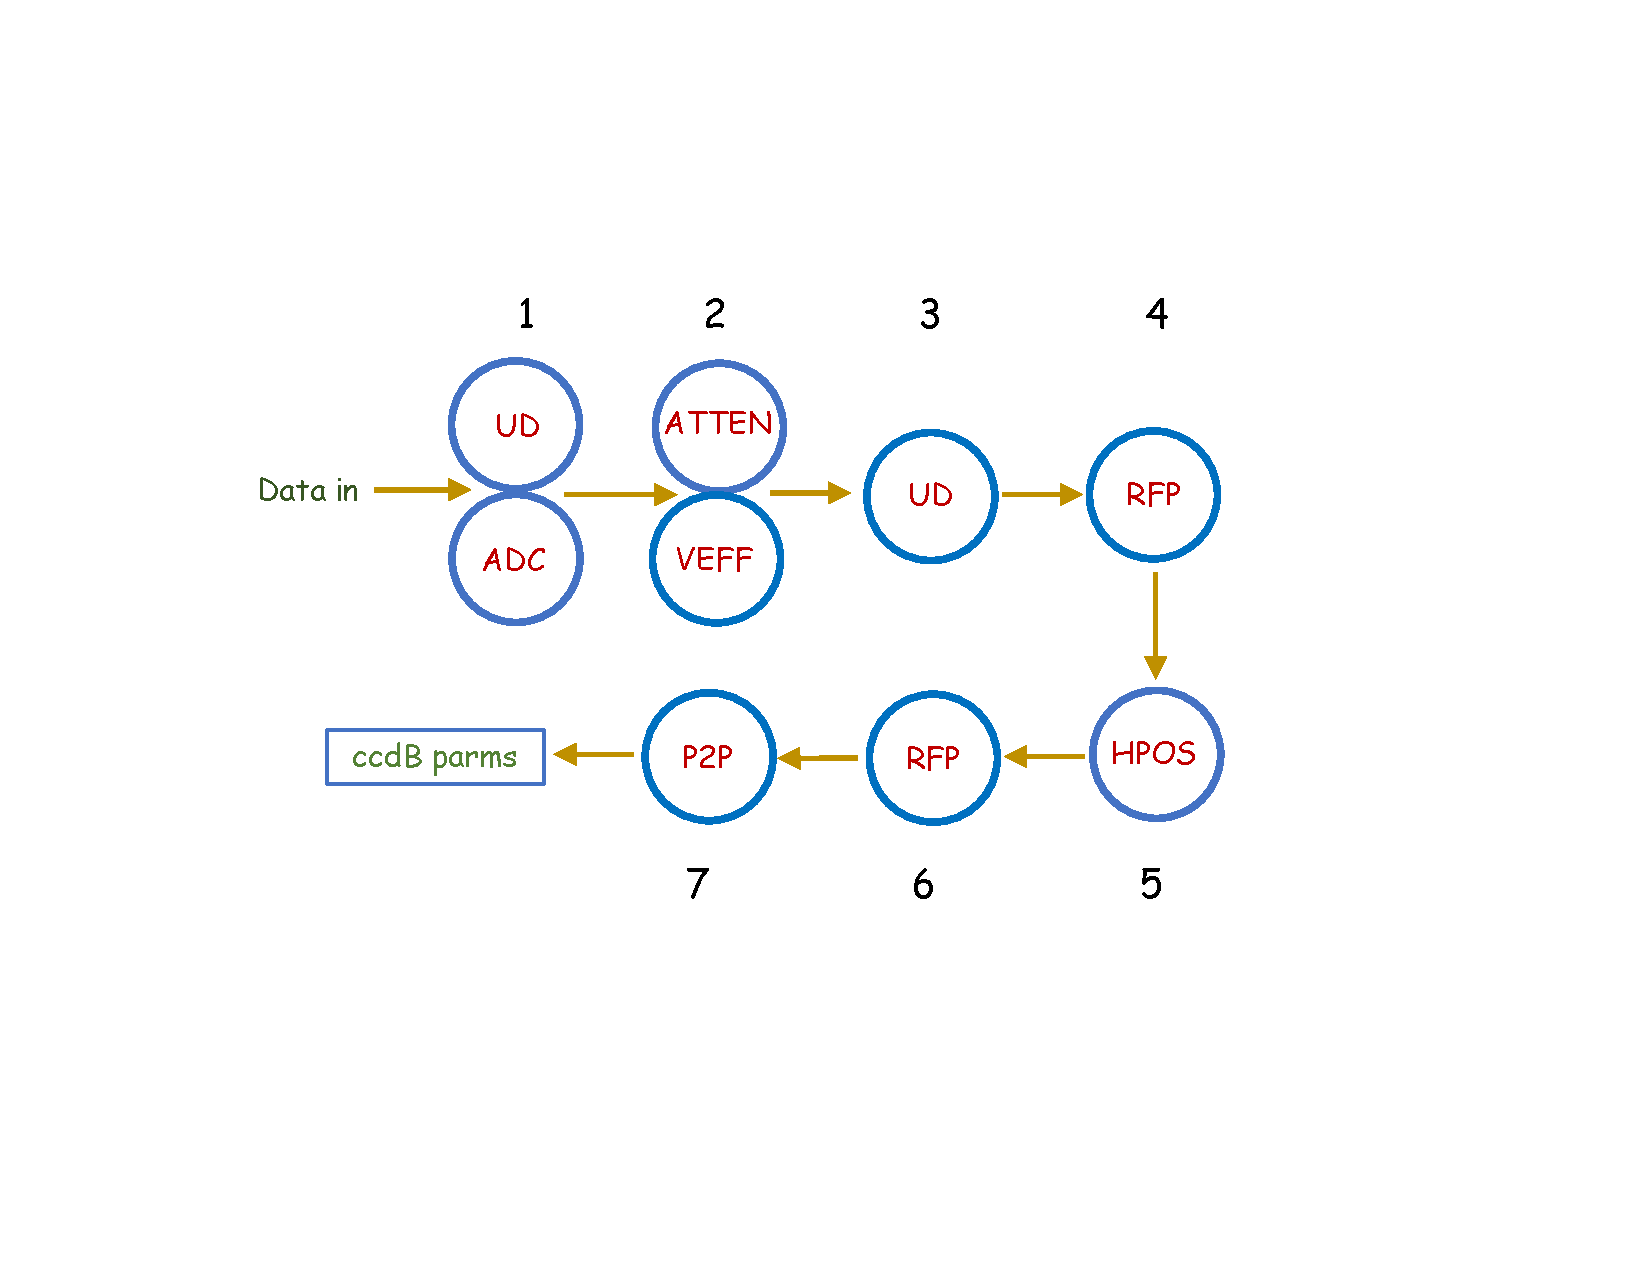
\includegraphics[width=0.55\textwidth,natwidth=610,natheight=642]{pics/calib-seq.pdf}}}
\end{picture} 
\caption{Schematic representation of the different steps in the CTOF calibration sequence and their
order.}
\label{calib-seq}
\end{figure}
%%%%%%%%%%%%%%%%%%%%%%%%%%%%%%%%%%%%%%%%%%%%%%%%%%%%%%%%%%%

The full calibration of each of the CTOF counters involves a number of discrete steps that are carried out
sequentially for a given data run (where a run typically lasts for about two hours of data collection). The
associated calibration constants for each run are stored in the CLAS12 calibration database (ccdB)
\cite{recon-nim}. After the calibration of a given data reference run is completed, the calibrations for
subsequent data runs are only carried out if there is a response shift outside of our allowed timing or energy
tolerances (which are typically 5\%). The steps to complete the CTOF calibration are carried out in a
particular sequence as detailed in Ref.~\cite{ctof-calib} and shown schematically in the calibration flowchart of
Fig.~\ref{calib-seq}. The individual steps include:

\begin{enumerate}
\item Upstream/downstream PMT time offsets (UD): This time offset accounts for the difference in the
time recorded between the upstream and downstream PMTs in a given counter due mainly to the different
signal cable lengths. These time offsets are determined from the centroid of the difference between the
upstream/downstream TDC time difference and the upstream/downstream hit times computed using the
counter hit point from the central tracking system divided by the effective speed of light in the counter.
These time offsets range between 25$\pm$5~ns. This step is carried out initially in order to compute a hit
coordinate from the CTOF information for the effective velocity determination and then a second time to
account for the fact that the effective velocity slightly shifts the time offset centroid.

\item ADC Calibration (ADC): Determine the ADC channel to energy deposition calibration factor for each
counter using minimum-ionizing events; see Section~\ref{gain-matching}.

\item Attenuation Length Calibration (ATTEN): Determine the practical attenuation length of the counters;
see Section~\ref{sec:attlen}.

\item Effective Velocity Calibration: Determine the effective speed of light propagation along the
counter; see Section~\ref{sec:veff}.

\item Counter-to-Counter Time Offset Calibration (RFP, P2P): In order to measure the absolute flight time
of a charged particle from the target to a CTOF counter and to be able to reconstruct exclusive events
when hits are associated with multiple CTOF counters, time offsets of each counter relative to all of the
other counters in the system need to be determined. This is done in two steps. The first step is to align each
counter hit time to the RF time, a step that amounts to a precision time alignment in bins of the TDC LSB. The
second step is a coarse alignment of each counter hit time in bins of the RF period $T_{RF}$; see
Section~\ref{sec-talign}. During this step the effective counter time resolutions are determined; see
Section~\ref{tres-beam}.

\item Hit Position-Dependent Time Correction (HPOS): Correct hit times for position-dependent shifts
associated with the curved ends of the scintillation bars; see Section~\ref{sec-hpos}.

\item TDC Calibration (TDC): After calibrating the integral non-linearities of each TDC channel in the system
(see Section~\ref{sec-elec}), the TDC channel to time calibration is completed using beam events; see
Section~\ref{sec-tdccal} for details and a note of why this step is not included on the Fig.~\ref{calib-seq}
flowchart.

\end{enumerate}

The calibration flowchart of Fig.~\ref{calib-seq} shows that the calibrations are completed in seven separate
calibration steps that proceed in series. The data run is analyzed to complete a given step and the determined
parameters are then used in the subsequent steps. Due to dependencies of the steps on each other, several
calibration steps (UD, RFP) have to be completed multiple times. As the CTOF calibration relies on accurate
determination of the event start time, which comes from the forward tracking system and the Forward
Time-of-Flight (FTOF) system~\cite{ftof-nim}, the calibrations of these subsystems are completed before
the CTOF calibrations in the overall CLAS12 subsystem calibration sequence.

To calibrate the CTOF system, events are selected that have a good electron reconstructed in the forward
direction as determined by the CLAS12 Event Builder (see Ref.~\cite{recon-nim} for details). The calibration
of CTOF relies on selecting tracks whose curvature in the solenoid field identifies them as negatively charged.
These tracks are overwhelmingly pions.

The average hit time resolution for the CTOF from the TDCs is $<$100~ps and that from the CTOF
FADCs, given the rapid fall time of the fast PMT signals that provide for only 2-3 samples on the falling
edge, is only $\sim$1~ns. A matching requirement of 10~ns between the TDC time and the FADC time is
employed during event reconstruction. While this matching requirement still needs to be tuned further,
at the current time it is already reasonably effective in allowing the FADC hits to be matched with their
corresponding TDC hits. This is important, as due to the slightly different thresholds on the discriminators
and the FADCs, the number of entries in the hit lists can be different. The matching criteria is also essential
in order to assign the correct ADC information to the hit for the proper energy deposition computation.

\subsubsection{PMT Gain Matching}
\label{gain-matching}

One of the purposes of gain-matching the CTOF PMTs is to equalize the detector response to tracks that
cross the barrel such that two counters are involved. This is a necessary procedure because each counter
must contribute equally to the trigger for a common-threshold discriminator level (see Ref.~\cite{trigger-nim}
for details on the CTOF within the trigger). Gain matching so that the minimum-ionizing particle peak appears
in the same ADC channel for all counters also allows for easier data monitoring during online and offline analysis.

The CTOF PMT high voltage settings were determined using calibration runs employing minimum-ionizing
tracks. These tracks deposit roughly 6~MeV as they pass through the 3-cm thick CTOF scintillation bars,
as $dE/\rho dx = 1.956$~MeV/g/cm$^2$ for minimum-ionizing particles. The initial high voltage settings
were based on runs using cosmic rays with the solenoid at zero field and a readout based on an event
selection that required tracks to cross the barrel to select tracks approximately perpendicular to the
face of the CTOF counters. This was done for each counter by selecting tracks within $\pm$1 bar about
the bar on the opposite side of the barrel. This selection was loose enough to allow all counters to be well
calibrated with data runs of $\sim$4~hr in duration. During production data taking, these calibrations are
carried out using minimum-ionizing tracks from beam data coming from the target. In this case the integral
of the ADC pulse is scaled by a path-length correction given by $t/p$, where $t$ is the counter thickness
and $p$ is the path-length of the track in the counter as determined by extrapolation of the track beyond
the central tracker to the location of the CTOF counter. The energy deposited in the scintillation bars is
recorded by the ADCs, which show Landau peaks above pedestal. Minimum-ionizing tracks that do not pass
through the full counter thickness and more heavily ionizing tracks give rise to a background beneath the
Landau peak.

For the HV calibrations, to avoid issues with the attenuation of light for tracks that pass near the ends of
the bars and with unbalanced light entering the upstream and downstream PMTs, we combine the
pedestal-subtracted ADC information from the upstream and downstream PMTs to produce an average
ADC spectrum for the counter through the quantity known as the geometric ADC mean:

\begin{equation}
\label{adc}
\overline{ADC} = \sqrt{ (ADC - PED)_U \cdot (ADC - PED)_D}.
\end{equation}

\noindent
Figure~\ref{gmean} shows the geometric mean spectrum for one representative CTOF counter using beam
data.

%%%%%%%%%%%%%%%%%%%%%%%%%%%%%%%%%%%%%%%%%%%%%%%%%%%%%%%%%
\begin{figure}[htbp]
\vspace{2.2cm}
\begin{picture}(30,50) 
\put(55,-27)
{\hbox{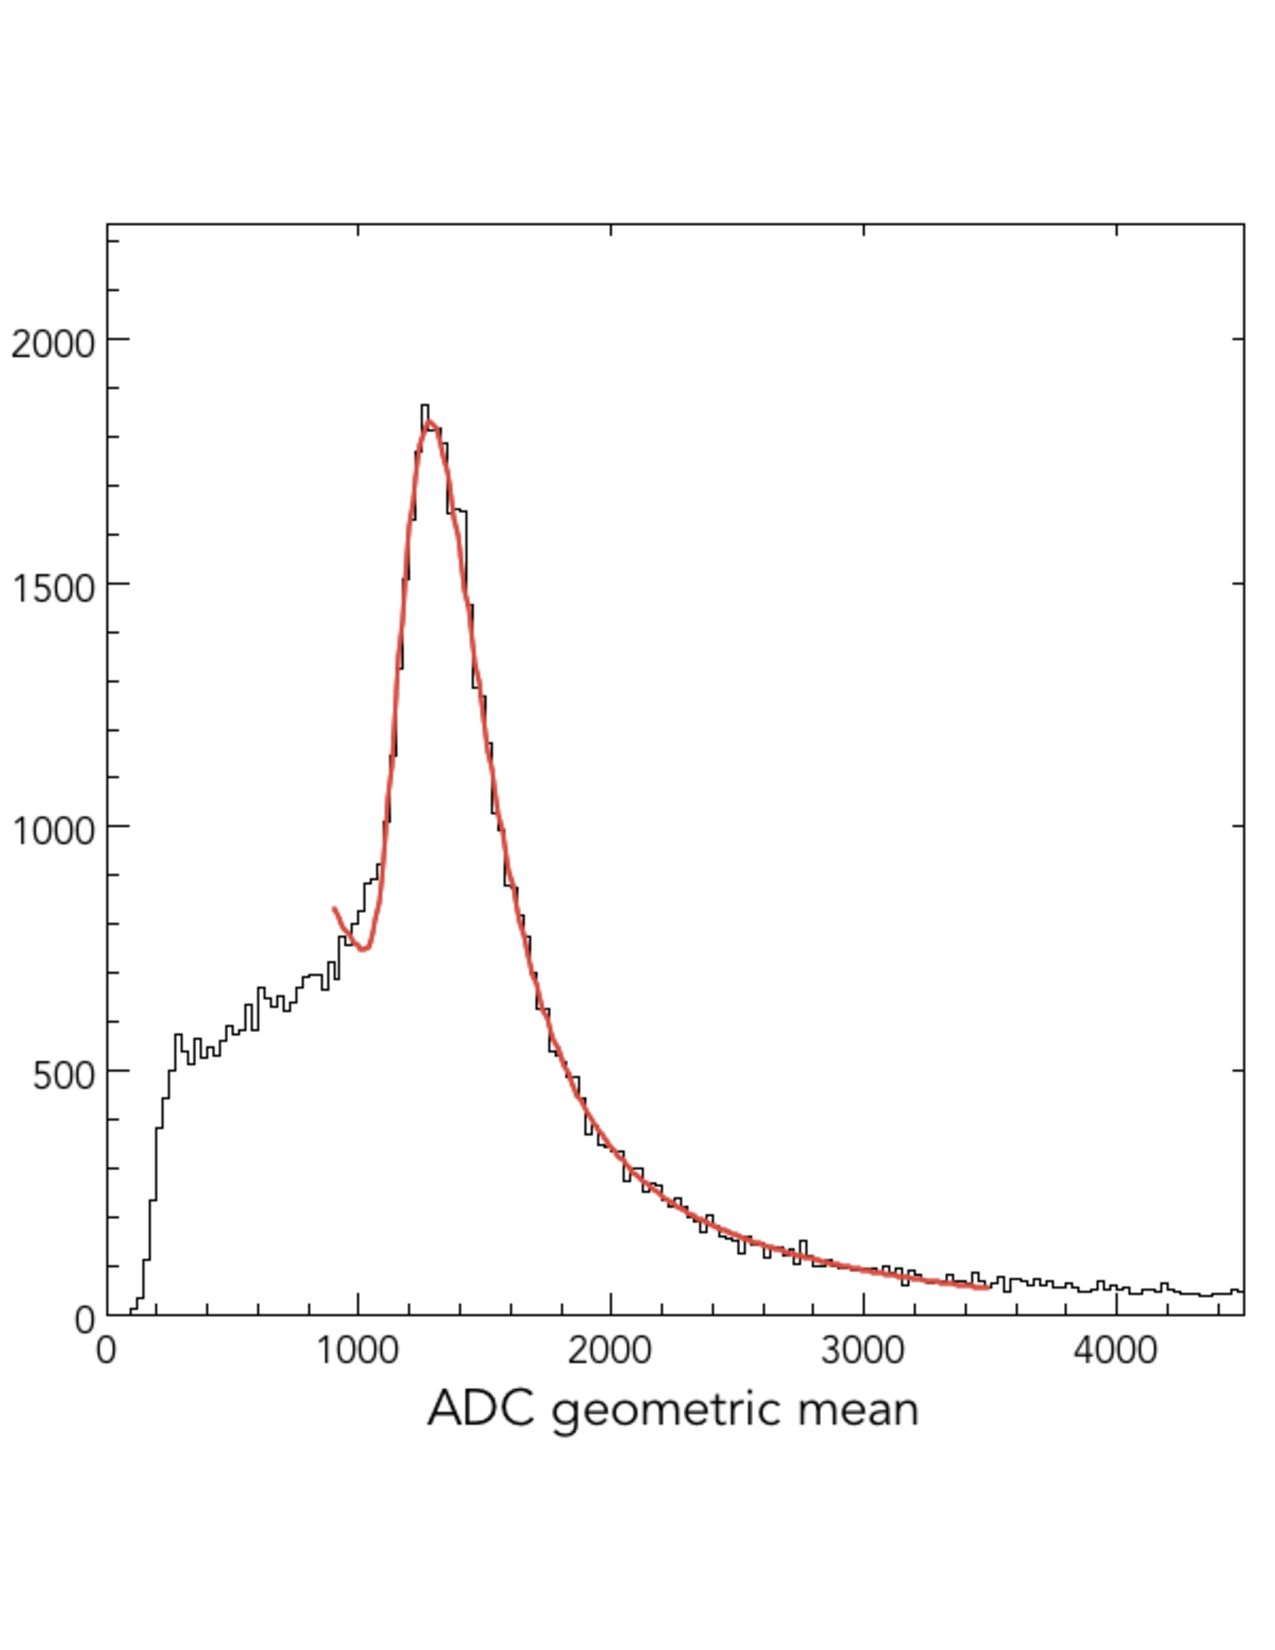
\includegraphics[width=0.25\textwidth,natwidth=610,natheight=642]{pics/gmean.pdf}}}
\end{picture} 
\caption{Geometric ADC mean spectrum for one representative CTOF counter from beam data. The events
recorded are pedestal subtracted. The red curve is a fit function that includes a Landau shape for the
peak and an exponential for the background.}
\label{gmean}
\end{figure}
%%%%%%%%%%%%%%%%%%%%%%%%%%%%%%%%%%%%%%%%%%%%%%%%%%%%%%%%%

Given the finite dynamic range of the ADC, we have chosen to position the minimum-ionizing peak in a
particular ADC channel that is selected so that it is safely above the pedestal, but leaves sufficient range
for the more highly ionizing charged tracks of our typical physics events. To minimize PMT aging effects
that result in loss of PMT gain with time correlated with the total charge collected at the anode of the
the PMT, the high voltages are set as low as possible.

The gain $G$ of a PMT can be related to the high voltage setting $V$ using $G \propto V^\alpha$, which
represents a basic power law form with $\alpha$ the power law factor.  This expression governs the gain
change for a given change in voltage. With this expression, the PMT gain $G_1$ at a given voltage $V_1$ can
be related to the gain $G_2$ at a different voltage $V_2$ using:

\begin{equation}
\label{power-law}
\frac{G_1}{G_2} = \left( \frac{V_1}{V_2} \right) ^\alpha,
\end{equation}

\noindent
which can be rewritten in a slightly different form as:

\begin{equation}
\label{delta}
\frac{\Delta G}{G} = \alpha \frac{\Delta V}{V}.
\end{equation}

\noindent
For our purposes we assume that the gain $G$ is directly proportional to the measured ADC value. With an
expression that relates the measured ADC value at two different voltage settings, we have a relation that
forms the basis for relating the position of the minimum-ionizing peak in the $\overline{ADC}$ spectrum
(see Eq.(\ref{adc})) to the PMT HV setting. The gain-matching procedure then amounts to adjusting the HV
settings of all PMTs to the values required to position the minimum-ionizing peak for each counter in the
desired ADC location. At the same time the algorithm uses the individual upstream and downstream PMT
ADC spectra for a given counter to ensure that the PMT gains for each counter are balanced. The iterative
process to determine the final set of PMT HV values typically converges in 1 to 2 data runs. For initial
operation of the PMTs we have chosen to center the minimum-ionizing peak in the $\overline{ADC}$ spectrum
for each counter in channel 900. 

The determination of the power law factor $\alpha$ in Eq.(\ref{power-law}) is important in order for the
HV calibrations to converge quickly. This factor can be determined directly from the data. For this purpose,
two data runs were acquired with different HV settings for the PMTs. After determining the locations of
the minimum-ionizing peaks from the ADC spectrum fits, Eq.(\ref{delta}) was used to solve for $\alpha$
for all PMTs. The average value from the data was determined to be $\alpha$=4.0$\pm$0.4 as shown in
Fig.~\ref{alpha-data}.

%%%%%%%%%%%%%%%%%%%%%%%%%%%%%%%%%%%%%%%%%%%%%%%%%%%%%%%%%
\begin{figure}[htbp]
\vspace{1.8cm}
\begin{picture}(50,50) 
\put(-15,-67)
{\hbox{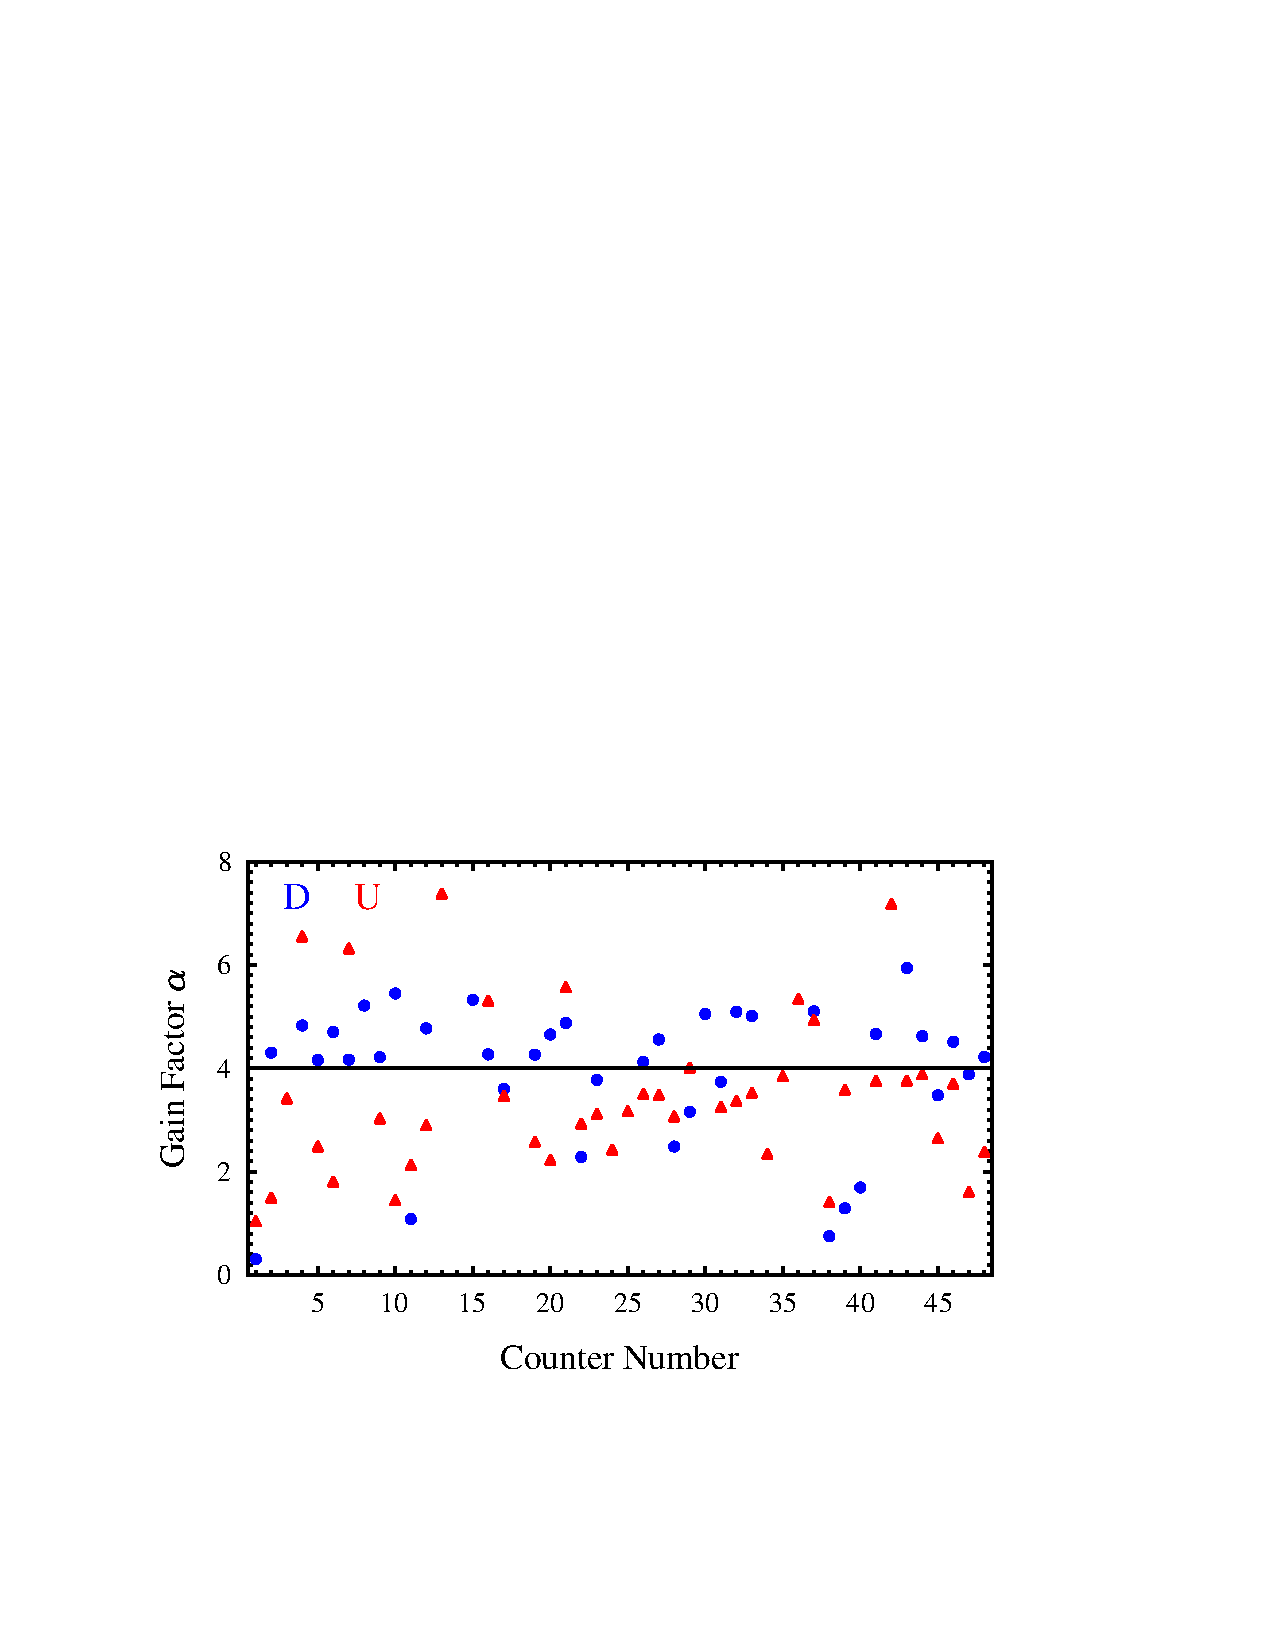
\includegraphics[width=0.58\textwidth,natwidth=610,natheight=642]{pics/alpha1.pdf}}}
\end{picture} 
\caption{Data showing the measurements of the power law factor $\alpha$ for each CTOF upstream PMT
(red triangles) and downstream PMT (blue circles). The average values of $\alpha$ is 4.}
\label{alpha-data}
\end{figure}
%%%%%%%%%%%%%%%%%%%%%%%%%%%%%%%%%%%%%%%%%%%%%%%%%%%%%%%%%

The energy loss in a counter for a passing charged particle track is determined after the
minimum-ionizing peak centroids are aligned. The energy loss in each counter is computed from each
PMT as:

\begin{equation}
E_{U,D} = ADC_{U,D} \cdot \left [ \frac{\left( \frac{dE}{dx} \right)_{MIP} \cdot t}{ADC_{MIP}}\right ]
\exp\left(\frac{d_{U,D}}{\lambda}\right),
\end{equation}

\noindent
where $ADC_{MIP}$ is the centroid of the minimum-ionizing peak in the geometric mean distribution,
$\left( \frac{dE}{dx} \right)_{MIP}$ is the energy loss for minimum-ionizing particles in the scintillation
bars (1.956~MeV/cm), $t$ is the counter thickness, $d$ is the distance along the bar from the track hit
position to the PMT, and $\lambda$ is the counter attenuation length. The energy loss used in the event
reconstruction is the mean of the separate $E_{U,D}$ measures (see Ref.~\cite{recon-nim} for details).

Figure~\ref{ctof-dedx} shows the reconstructed energy loss normalized by the track path length through
the bar for all counters from a data run with a 10.6~GeV electron incident upon a liquid-hydrogen target. The
data allow the separation of minimum-ionizing particles from more heavily ionizing particles. The minimum-ionizing
particles lose a constant energy as a function of path length. At low-momentum the more heavily ionizing
particles have energy loss that increases linearly with distance until they can pass through the counter. At
that point their energy loss follows the Bethe-Bloch formula.

%%%%%%%%%%%%%%%%%%%%%%%%%%%%%%%%%%%%%%%%%%%%%%%%%%%%%%%%%
\begin{figure}[htbp]
\vspace{2.1cm}
\begin{picture}(50,50) 
\put(0,140)
{\hbox{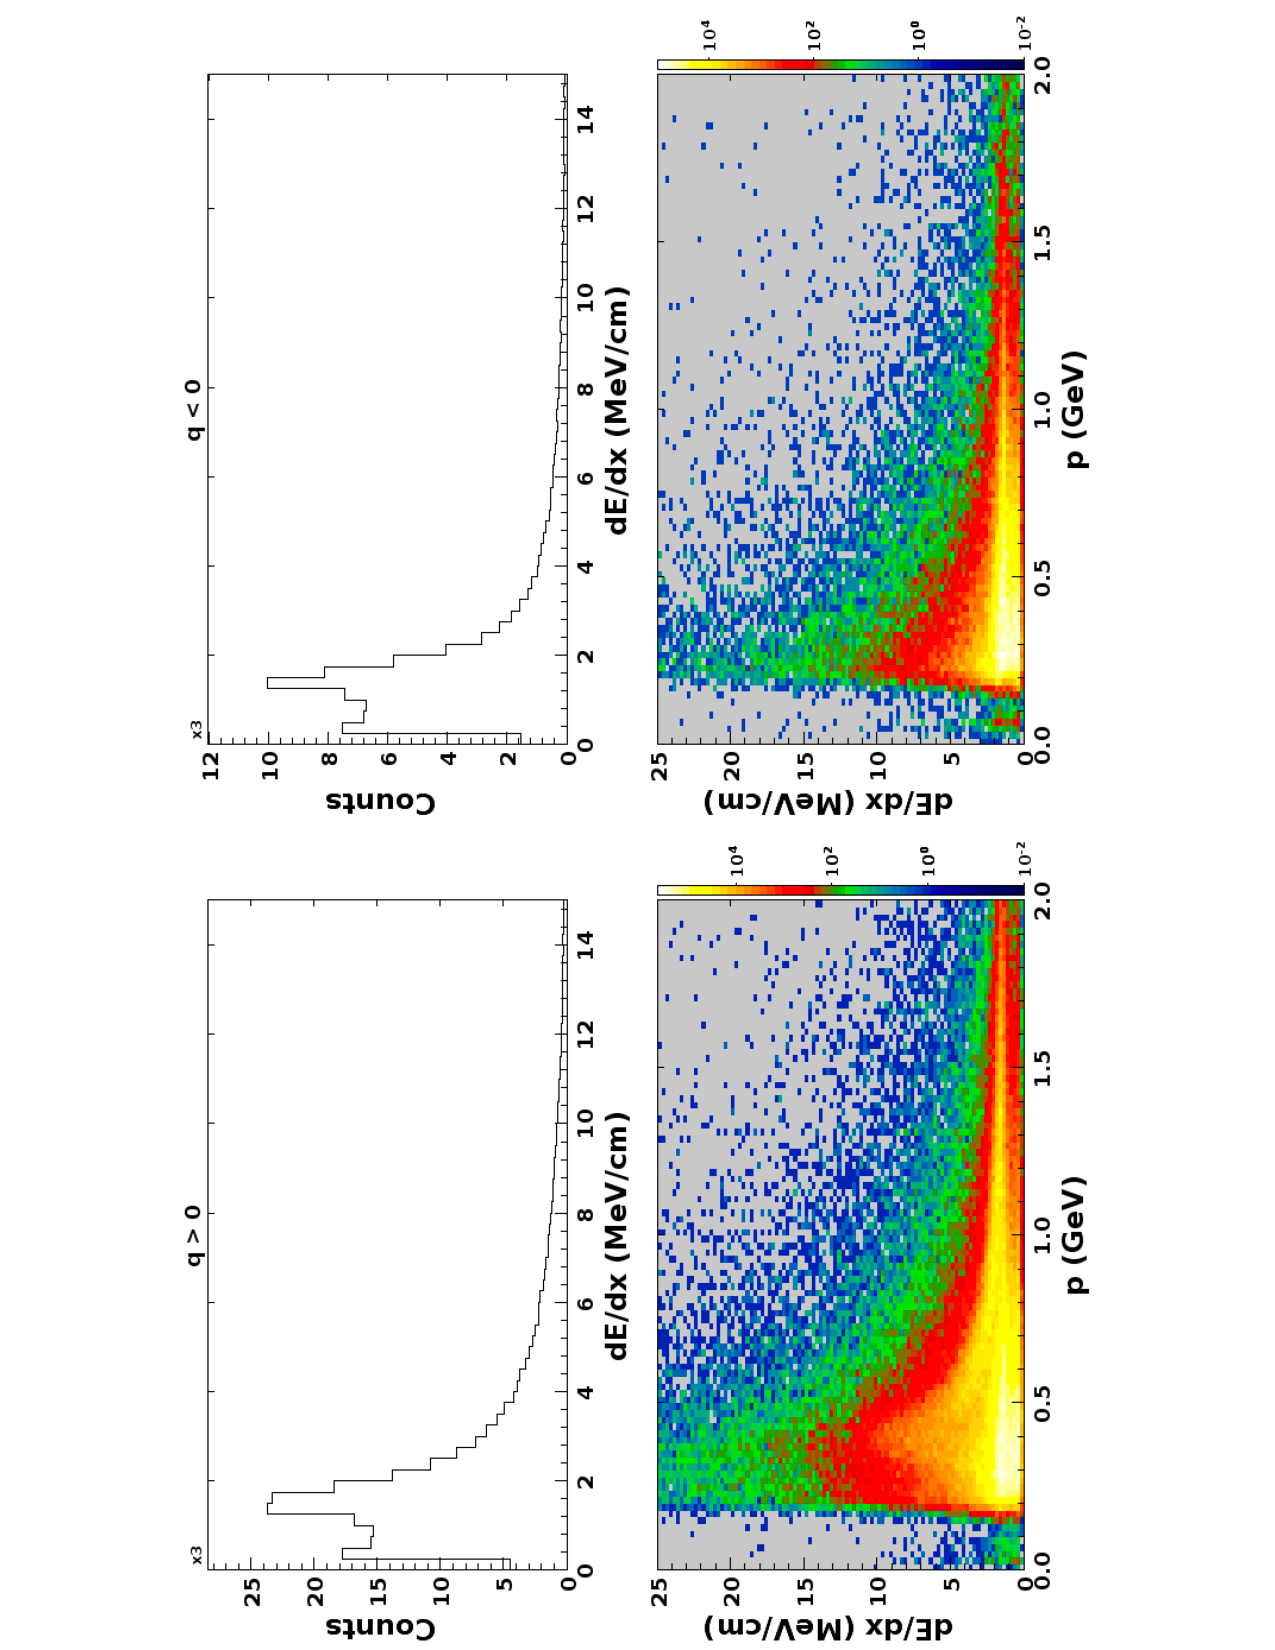
\includegraphics[width=0.37\textwidth,natwidth=610,natheight=642,angle=-90]
{pics/ctof-dedx.pdf}}}
\end{picture} 
\caption{Measured CTOF energy loss summed over all counters for positively (left column) and negatively
charged particles (right column) from 10.6-GeV electrons incident upon a liquid-hydrogen target normalized
by the extrapolated path length through the bar from the projection of the central track through the CTOF
barrel. The top row of plots show the normalized $dE/dx$ and the bottom row of plots show $dE/dx$ vs.
track momentum (GeV).}
\label{ctof-dedx}
\end{figure}
%%%%%%%%%%%%%%%%%%%%%%%%%%%%%%%%%%%%%%%%%%%%%%%%%%%%%%%%

\subsubsection{Attenuation Length Measurements}
\label{sec:attlen}

The measured ADC values for each PMT can be written in terms of the attenuation length as:

\begin{equation}
\label{al-adc}
(ADC - PED) = A_0 e^{-d/\lambda},
\end{equation}

\noindent
where $A_0$ is a constant, $d$ is the distance along the counter with respect to the PMT location, and
$\lambda$ is the counter attenuation length. Using the relation

\begin{equation}
d_{U/D} = \frac{L}{2} \pm coor,
\end{equation}

\noindent
where $L$ is the counter length, $coor$ is the CTOF hit coordinate along the bar (with the middle of the bar
at $coor=0$) defined as:

\begin{equation}
\label{coor}
coor = \frac{v_{eff}}{2} \cdot (t_U - t_D - C_{UD}),
\end{equation}

\noindent
$v_{eff}$ is the effective velocity of light in the scintillation bars (see Section~\ref{sec:veff} for details), and
$C_{UD}$ is the offset that centers the time difference distribution about 0.

The logarithmic ratio of the ADCs of the upstream and downstream PMTs from a given counter as a function of
hit coordinate along the bar can be written as:
\begin{equation}
\label{linear}
\log \left( \frac{(ADC-PED)_U}{(ADC-PED)_D} \right ) = C + \frac{2 \cdot coor}{\lambda}.
\end{equation}

\noindent
This expression can be used to determine the effective counter attenuation length using a linear fit of the
logarithmic ADC ratio vs. $coor$. The slope of this correlation is $2/\lambda$. In this expression, the
$y$-intercept $C$ is a constant given by $\log(A_0^U/A_0^D)$. Figure~\ref{atten-len1} shows the measured
attenuation lengths for the CTOF counters, whose average is found to be 140~cm in accord with expectations. 

%%%%%%%%%%%%%%%%%%%%%%%%%%%%%%%%%%%%%%%%%%%%%%%%%%%%%%%%%
\begin{figure}[htbp]
\vspace{2.0cm}
\begin{picture}(30,50) 
\put(12,-150)
{\hbox{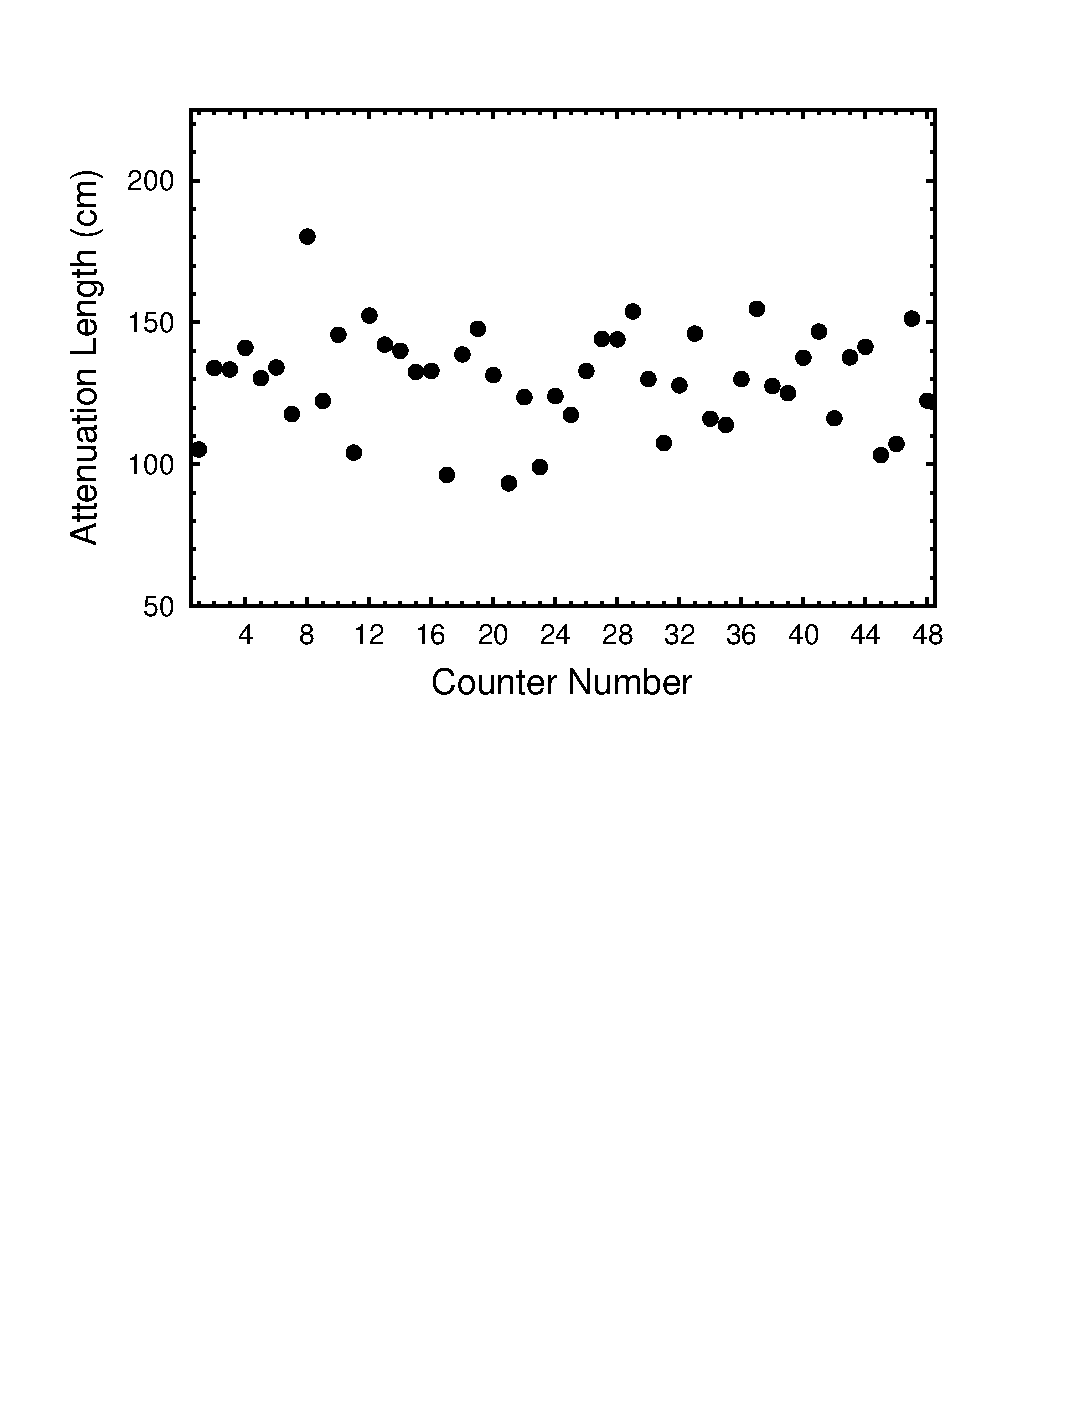
\includegraphics[width=0.53\textwidth,natwidth=610,natheight=642]{pics/atten.pdf}}}
\end{picture} 
\caption{Counter attenuation lengths (cm) vs. counter number determined from beam data.}
\label{atten-len1}
\end{figure}
%%%%%%%%%%%%%%%%%%%%%%%%%%%%%%%%%%%%%%%%%%%%%%%%%%%%%%%%%

\subsubsection{Effective Velocity Determination}
\label{sec:veff}

The effective velocity of light in each counter employs a calculation based on the comparison of the
reconstructed coordinate information along the scintillation bar from the TDC time information with the
track hit coordinate determined from the extrapolation of the track beyond the central tracker to the
location of the CTOF counters. Figure~\ref{veff} shows the measured effective velocity for each CTOF
counter using data with a 10.6-GeV electron beam incident upon a liquid-hydrogen target. The average
effective velocity is found to be 14.5~cm/ns.

%%%%%%%%%%%%%%%%%%%%%%%%%%%%%%%%%%%%%%%%%%%%%%%%%%%%%%%%%
\begin{figure}[htbp]
\vspace{2.0cm}
\begin{picture}(30,50) 
\put(20,-140)
{\hbox{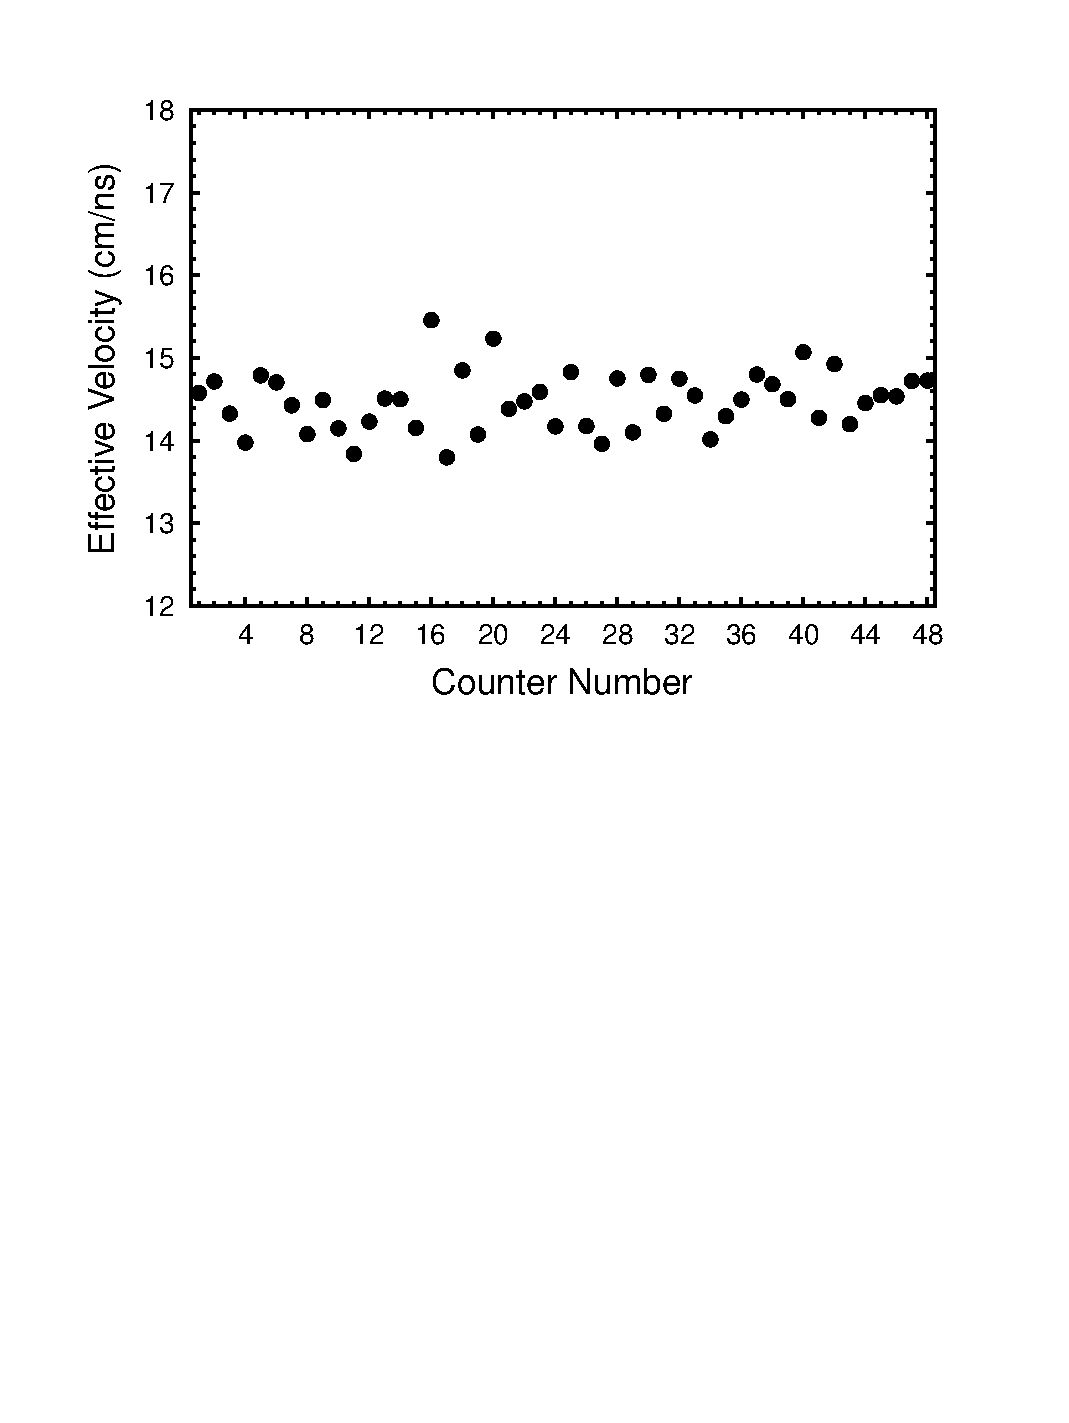
\includegraphics[width=0.50\textwidth,natwidth=610,natheight=642]{pics/veff.pdf}}}
\end{picture} 
\caption{Counter effective velocities (cm/ns) vs. counter number determined from beam data.}
\label{veff}
\end{figure}
%%%%%%%%%%%%%%%%%%%%%%%%%%%%%%%%%%%%%%%%%%%%%%%%%%%%%%%%%

\subsubsection{Counter-to-Counter Time Alignment}
\label{sec-talign}

The flight time of a charged particle from the reaction vertex to a CTOF counter is given by:

\begin{equation}
t_p = \overline{t}_{hit} - t_{ST},
\end{equation}

\noindent
where $\overline{t}_{hit}$ is the average CTOF counter hit time (using $t_U$ and $t_D$) and $t_{ST}$
is the event start time. The event start time is associated with the RF but needs to be synchronized
with the particular RF beam bucket associated with the event. The beam bunch width within the RF beam
bucket is only $\sim$2~ps and, therefore, represents a precise time marker. However, as the RF time
signal has a period of $T_{RF}$, it is not a priori known which RF beam bucket was the one associated with
the event that led to the hit in the CTOF counter.

The determination of the absolute flight time of charged particle tracks from the reaction vertex to the
CTOF counters is performed in two steps. In the first step, fine time offsets (binned in the 25~ps TDC
LSB) are determined to align the CTOF hit times within the RF time window. In the second step, coarse
time offsets binned in units of the RF period $T_{RF}$ are determined to select the specific RF beam
bucket associated with the event.

The fine time alignment algorithm (referred to as RFP) uses the CTOF hit time traced to the event vertex
relative to the start time to align the vertex times of all CTOF hits (modulo $T_{RF}$). This algorithm uses
the average counter hit times, 
\begin{eqnarray}
t_{res}' = mod \left[ t_{vtx}, T_{RF} \right], ~~~~~\\ [1ex]
t_{vtx} = \left(\overline{t}_{hit} - \frac{P_L}{\beta c} \right) - 
\left(t_{RF} + \frac{z_{vert}}{\beta_e c} \right). \nonumber
\end{eqnarray}

\noindent
The term $z_{vert}/(\beta_e c)$ shifts the start time to the actual event vertex location along the
$z$-axis of the extended target and $P_L/(\beta c)$ represents the particle flight time based on the
path length $P_L$ from the event vertex to the CTOF counter (from central tracking information
extrapolated to the location of the CTOF hit) and the speed $v$ of the particle as $\beta c = v$.

Figure~\ref{rfp-plot} shows the $t_{res}'$ distribution for one representative CTOF counter. The
centroid of the Gaussian fit gives the fine time offset. The width of the Gaussian fit represents
a measure of the effective time resolution of the counter. To display the full $t_{res}'$ distribution
avoiding any wrap-around effects near the edges of the $T_{RF}$ range, the algorithm plots the
$t_{res}'$ distribution in a range of $\pm T_{RF}/2$ about the peak channel in the distribution.

%%%%%%%%%%%%%%%%%%%%%%%%%%%%%%%%%%%%%%%%%%%%%%%%%%%%%%%%%%
\begin{figure}[htbp]
\vspace{1.7cm}
\begin{picture}(50,50) 
\put(40,-45)
{\hbox{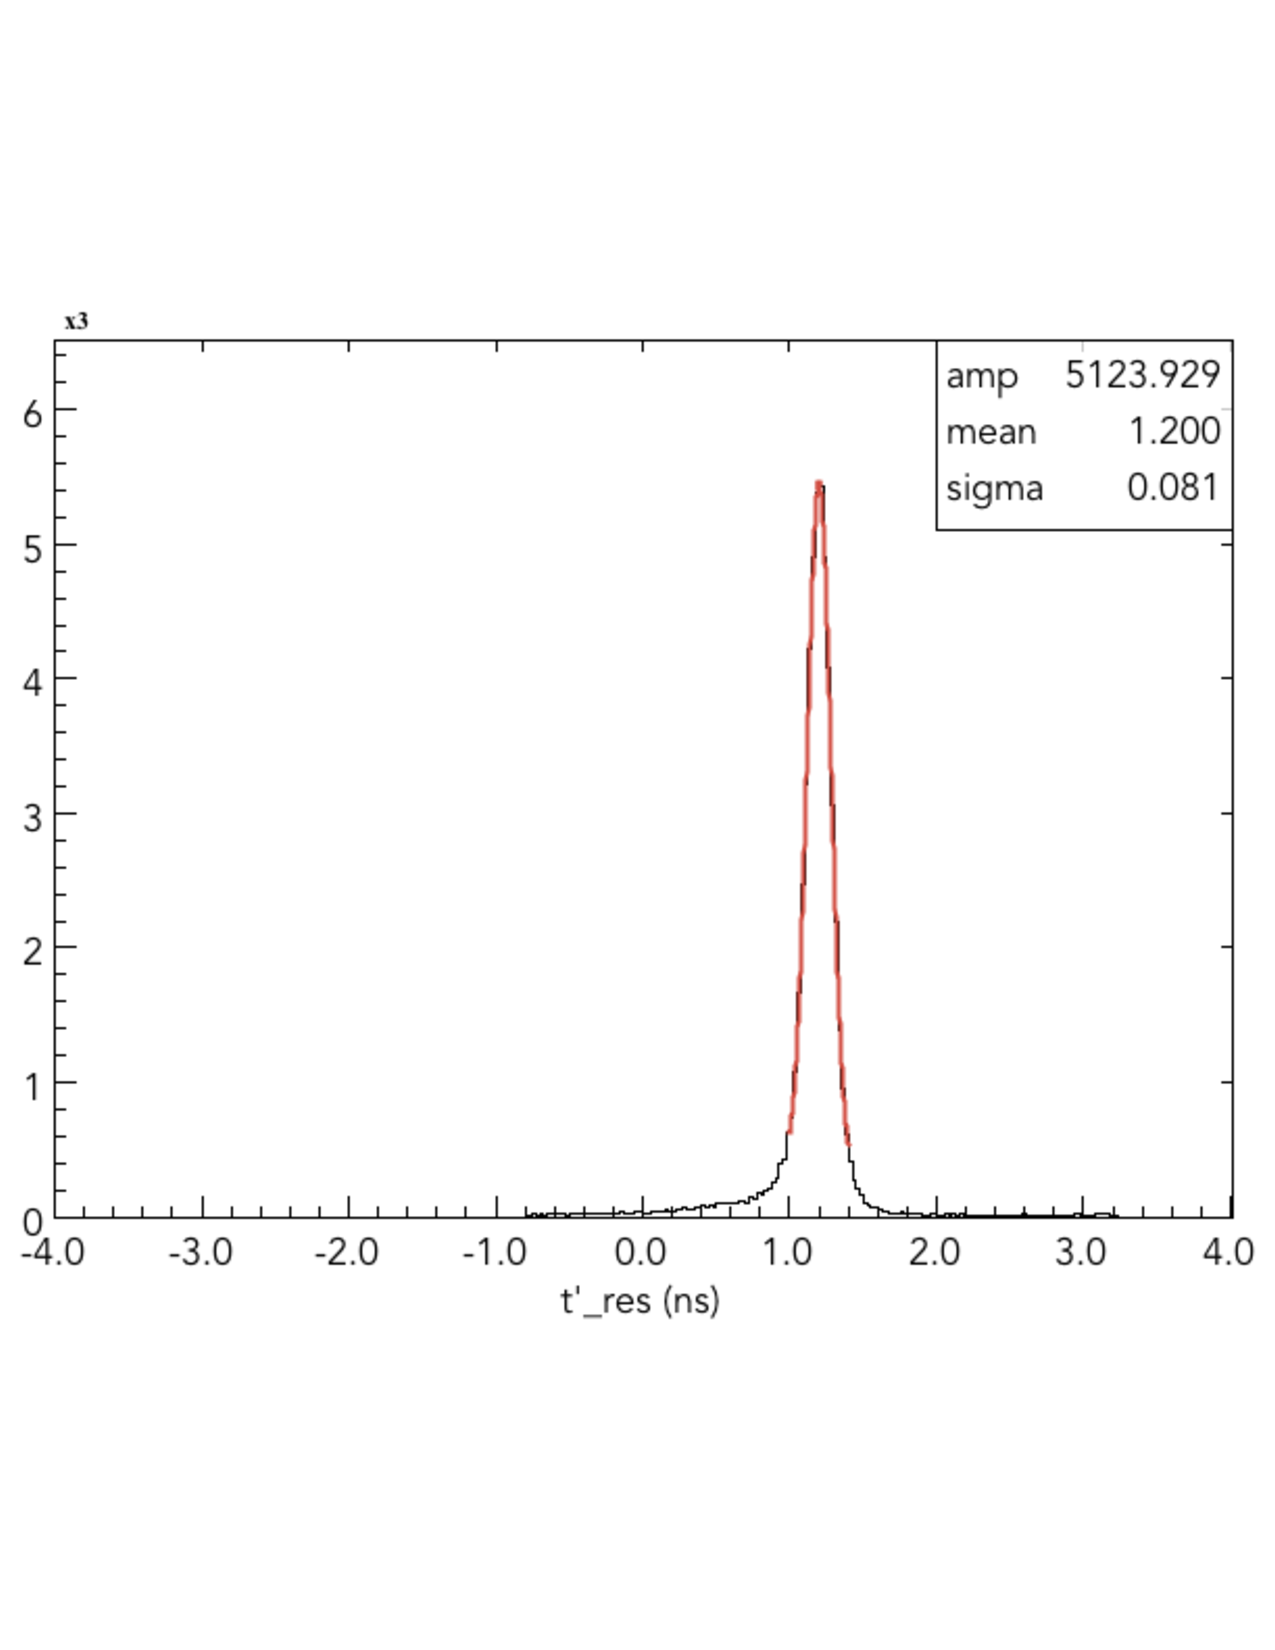
\includegraphics[width=0.30\textwidth,natwidth=610,natheight=642]{pics/rfp-plot.pdf}}}
\end{picture} 
\caption{Distribution of the CTOF hit times from beam data traced back to the vertex relative to the
RF (ns) for one representative CTOF counter with the Gaussian plus background fit overlaid to determine
the counter RF offset and the effective counter time resolution.}
\label{rfp-plot}
\end{figure}
%%%%%%%%%%%%%%%%%%%%%%%%%%%%%%%%%%%%%%%%%%%%%%%%%%%%%%%%%%

After the fine time offset calibration, the counter time is precisely aligned modulo $T_{RF}$. The next
step in the CTOF time calibration is to fix the measured hit times for all counters to the specific RF bunch
associated with the event. These coarse time offsets (called P2P for paddle-to-paddle) are determined
using coincidences of charged particle tracks in CLAS12 with one track in the forward direction hitting a
counter in the FTOF system and one track in the central detector hitting a CTOF counter. The offsets for
each CTOF counter $i$ ($i = 1 \to 48$) are computed using the time difference:

\begin{equation}
t_{P2P} = t_{vert}^i - t_{ST},
\end{equation}

\noindent
where,

\begin{equation}
t_{vert}^i = \overline{t}_{hit}^i - \frac{P_L}{\beta c}.
\end{equation}

\noindent
Here $t_{ST}$ is the event start time determined using a forward-going scattered electron from the
event reconstruction or, if there is no electron, a forward-going high momentum charged pion. The event
start time is determined using the forward tracking and FTOF systems. Therefore, the CTOF time
calibrations can proceed only after the calibrations of these other systems have been completed. The
algorithm adjusts the vertex time differences over all counters to set them to zero. The coarse time
offsets represents a single parameter for each counter that is restricted to values of $n \cdot T_{RF}$,
with $n = 0, \pm 1, \pm 2, ...$. As these constants are predominantly determined by the fixed system
cable lengths, the constants primarily reflect the differences in the signal propagation times along the
signal cables.

\subsubsection{Hit Position-Dependent Time Correction}
\label{sec-hpos}

The determination of the charged particle path lengths for tracks passing through the straight section
of the bar (see Fig.~\ref{scint-geom}) is straightforward. Our algorithm defines the track end point to
be in the middle of the bar. However, for tracks that enter into the curved portion of the bar at its
downstream end, the assignment of the track end point is uncertain as the effective thickness of the bar
as seen by charged tracks in this region can be up to 7-8~cm. Our approach is to define the end point for
all tracks in the CTOF to be on the surface of a cylinder through the middle of the straight section of the
bars. This introduces an artifact in $t'_{res}$ vs. hit position along the bar. To remove this effect (see
Fig.~\ref{hpos}(left)), we fit the data with an ad hoc functional of the form:

\begin{equation}
\delta t_{hpos} = a + b e^{cx},
\end{equation}

\noindent
where $a$, $b$, and $c$ are the fit constants for each counter. Figure~\ref{hpos} shows the vertex time
before and after subtracting $\delta t_{hpos}$ in the HPOS algorithm step.

%%%%%%%%%%%%%%%%%%%%%%%%%%%%%%%%%%%%%%%%%%%%%%%%%%%%%%%%%%
\begin{figure}[htbp]
\vspace{0.8cm}
\begin{picture}(50,50) 
\put(-58,-103)
{\hbox{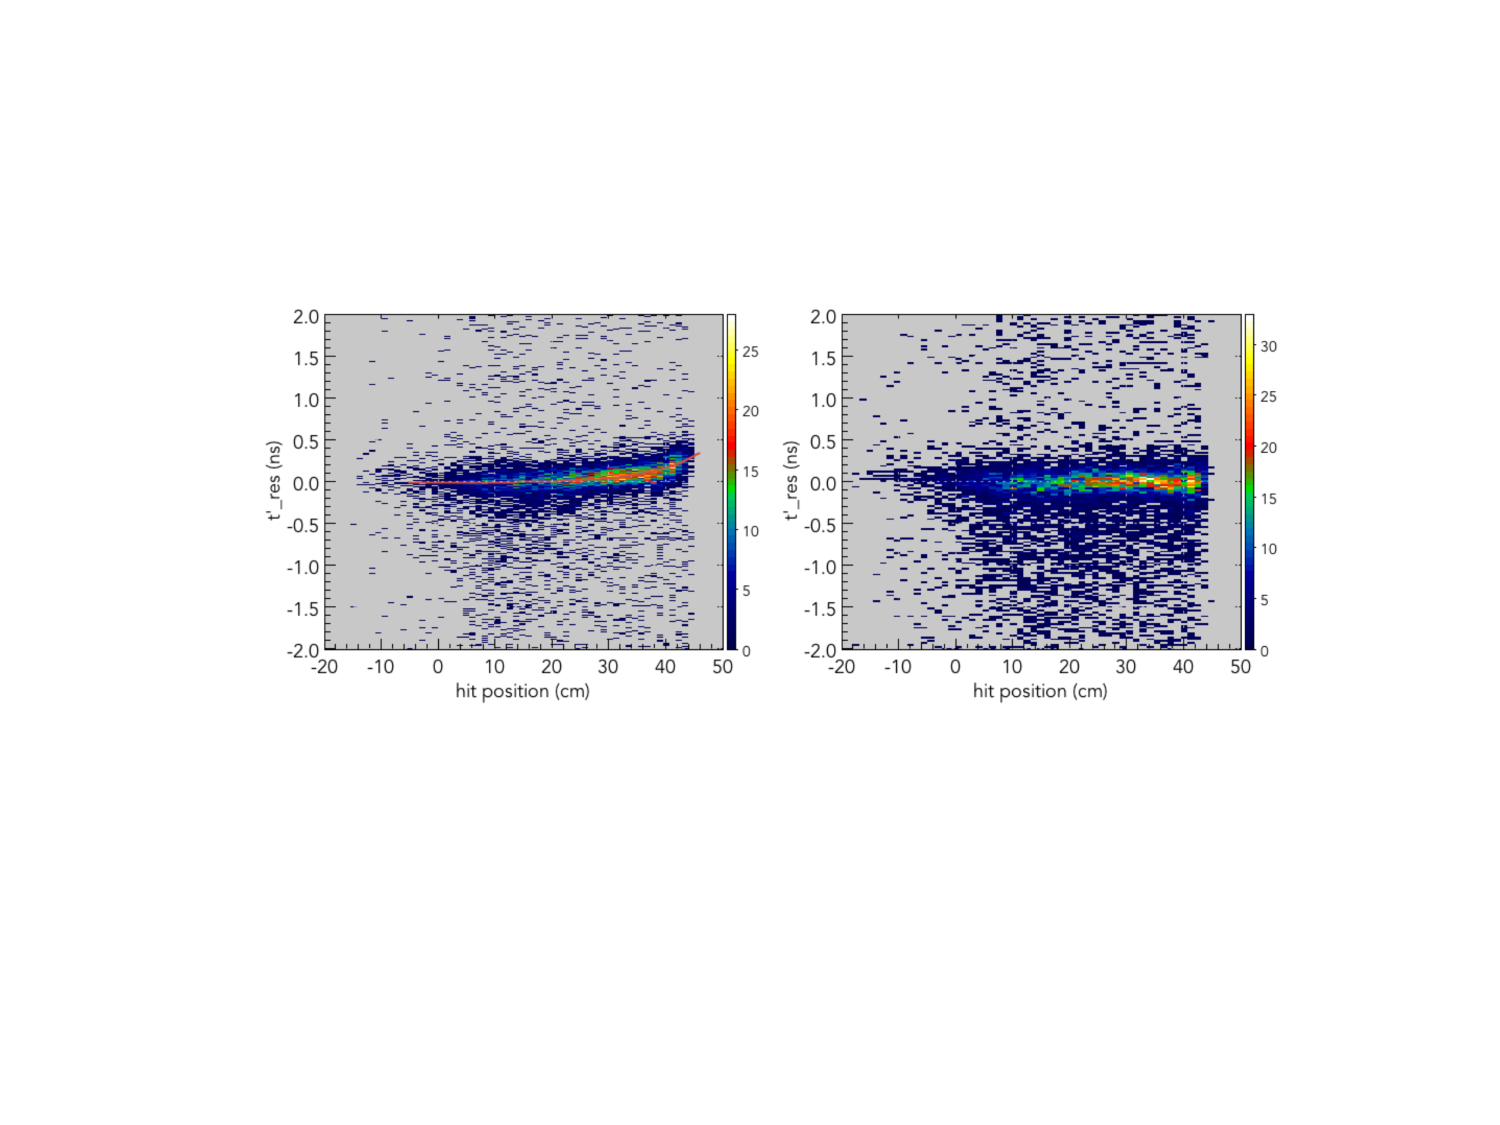
\includegraphics[width=0.60\textwidth,natwidth=610,natheight=642]{pics/hpos.pdf}}}
\end{picture} 
\caption{Distribution of $t_{res}'$ (ns) vs. hit position along the bar (cm) (left) before and (right) after
the hit position-dependent correction. The left plot shows the fit functional overlaid on the data for a
representative CTOF counter.}
\label{hpos}
\end{figure}
%%%%%%%%%%%%%%%%%%%%%%%%%%%%%%%%%%%%%%%%%%%%%%%%%%%%%%%%%%

\subsubsection{TDC Calibration}
\label{sec-tdccal}

The final step is the calibration of the TDCs. This calibration is a single constant for each TDC channel in the
system that converts the measured TDC channel bin into time. The nominal TDC LSB is 25~ps for the CAEN
VX1290N TDC units employed for the CTOF readout (see Section~\ref{sec-elec}).

The calibration is completed by fitting the PMT time residuals vs. TDC channel separately for the times
from the upstream and downstream PMTs using a linear function. The TDC calibration is the value that
fixes the slope of $t_{res}'$ vs. TDC to be zero. Figure~\ref{tdc-plot} shows the distribution of $t_{res}'$
vs. TDC for a representative CTOF PMT. Any bin-to-bin $\Delta t$ variations reflect remaining integral
non-linearities in the measured TDC compensation tables. At the present time a single conversion constant
of CONV = 23.45~ps/bin is employed for all CTOF system TDC input channels. This value is derived using a TDC
channel that digitizes the RF time (our most accurate time reference in Hall~B). For this reason individual
TDC channel calibrations are not shown as a separate step in Fig.~\ref{calib-seq} an the channel-by-channel
TDC calibrations done for CTOF serve only as a cross-check.

%%%%%%%%%%%%%%%%%%%%%%%%%%%%%%%%%%%%%%%%%%%%%%%%%%%%%%%%%%
\begin{figure}[htbp]
\vspace{2.4cm}
\begin{picture}(50,50) 
\put(35,-52)
{\hbox{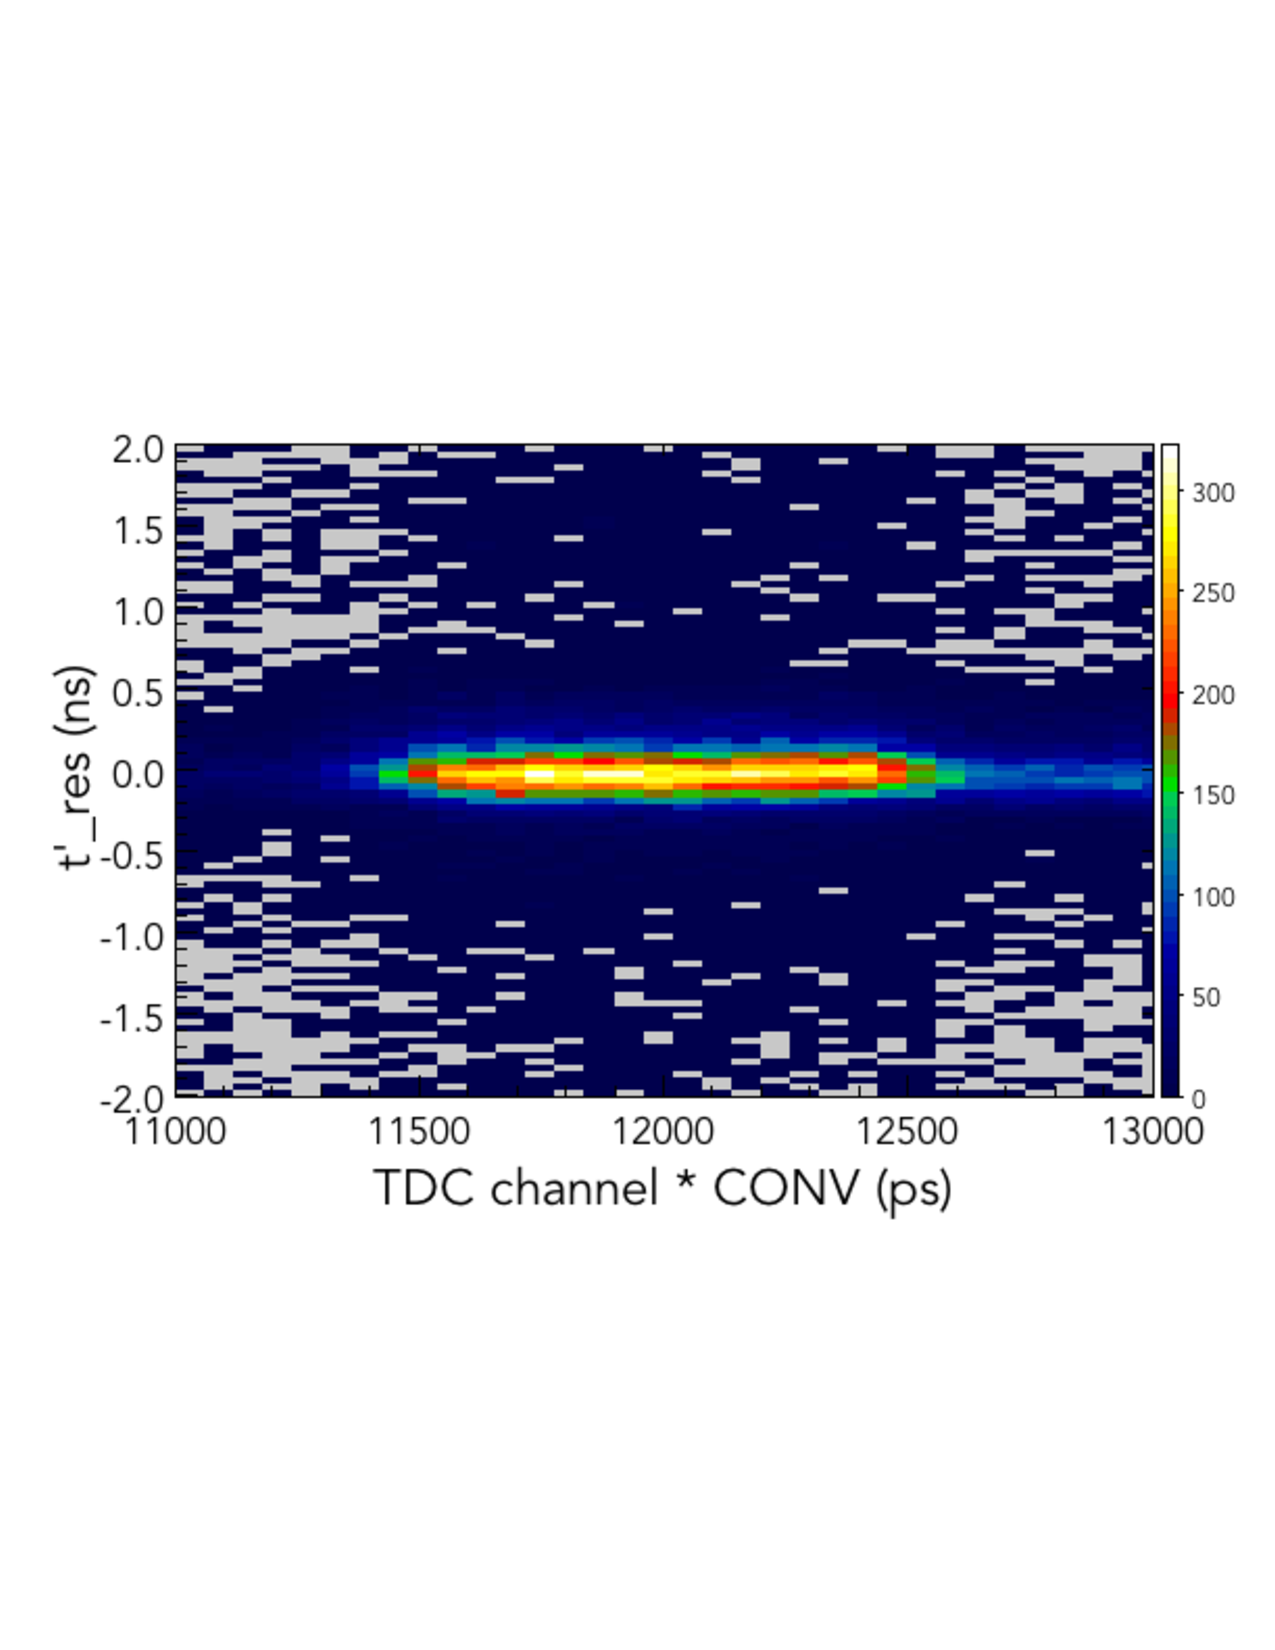
\includegraphics[width=0.35\textwidth,natwidth=610,natheight=642]{pics/tdc-plot.pdf}}}
\end{picture} 
\caption{Distribution of $t_{res}'$ (ns) vs. TDC channel * CONV (ps) for one representative CTOF PMT.
The TDC conversion constant for each channel is that which forces the slope of a linear fit to be zero.}
\label{tdc-plot}
\end{figure}
%%%%%%%%%%%%%%%%%%%%%%%%%%%%%%%%%%%%%%%%%%%%%%%%%%%%%%%%%%

\subsubsection{Counter Time Resolutions}
\label{tres-beam}

The effective time resolutions for each counter determined during the fine time alignment step
discussed in Section~\ref{sec-talign} are shown in Fig.~\ref{eff-tres}. These measurements were
taken after complete calibrations of the CTOF system from a beam data run with 10.6~GeV electrons
incident upon a liquid-hydrogen target. The time resolution displayed here represents the quality of the
overall CLAS12 calibrations at the current time. The results are based on calibration procedures that
are not yet fully optimized, as well as uncertainties in the momentum, track path length, and event vertex
from the forward and central track reconstruction. It is also important to mention that studies of the
CLAS12 subsystem detector alignment based on survey data and zero-field straight track data are in
progress. Misalignments of the detector affect the quality and accuracy of the reconstruction. When these
smearing effects are ultimately accounted for the timing resolution is expected to further improve.

Nevertheless, the average effective counter time resolutions already achieved of 85~ps are close to system
design specifications of 80~ps outlined in Section~\ref{sec:overview} and shown in Table~\ref{spec-table}.
With these resolutions, the quality of the particle identification in the Central Detector of CLAS12 allows the
experimental program in Hall~B to reach its goals. As further operating experience with CLAS12 is gained, we
expect to realize further modest but important improvements in the CTOF time resolution.

%%%%%%%%%%%%%%%%%%%%%%%%%%%%%%%%%%%%%%%%%%%%%%%%%%%%%%%%%
\begin{figure}[htbp]
\vspace{1.8cm}
\begin{picture}(50,50) 
\put(20,-140)
{\hbox{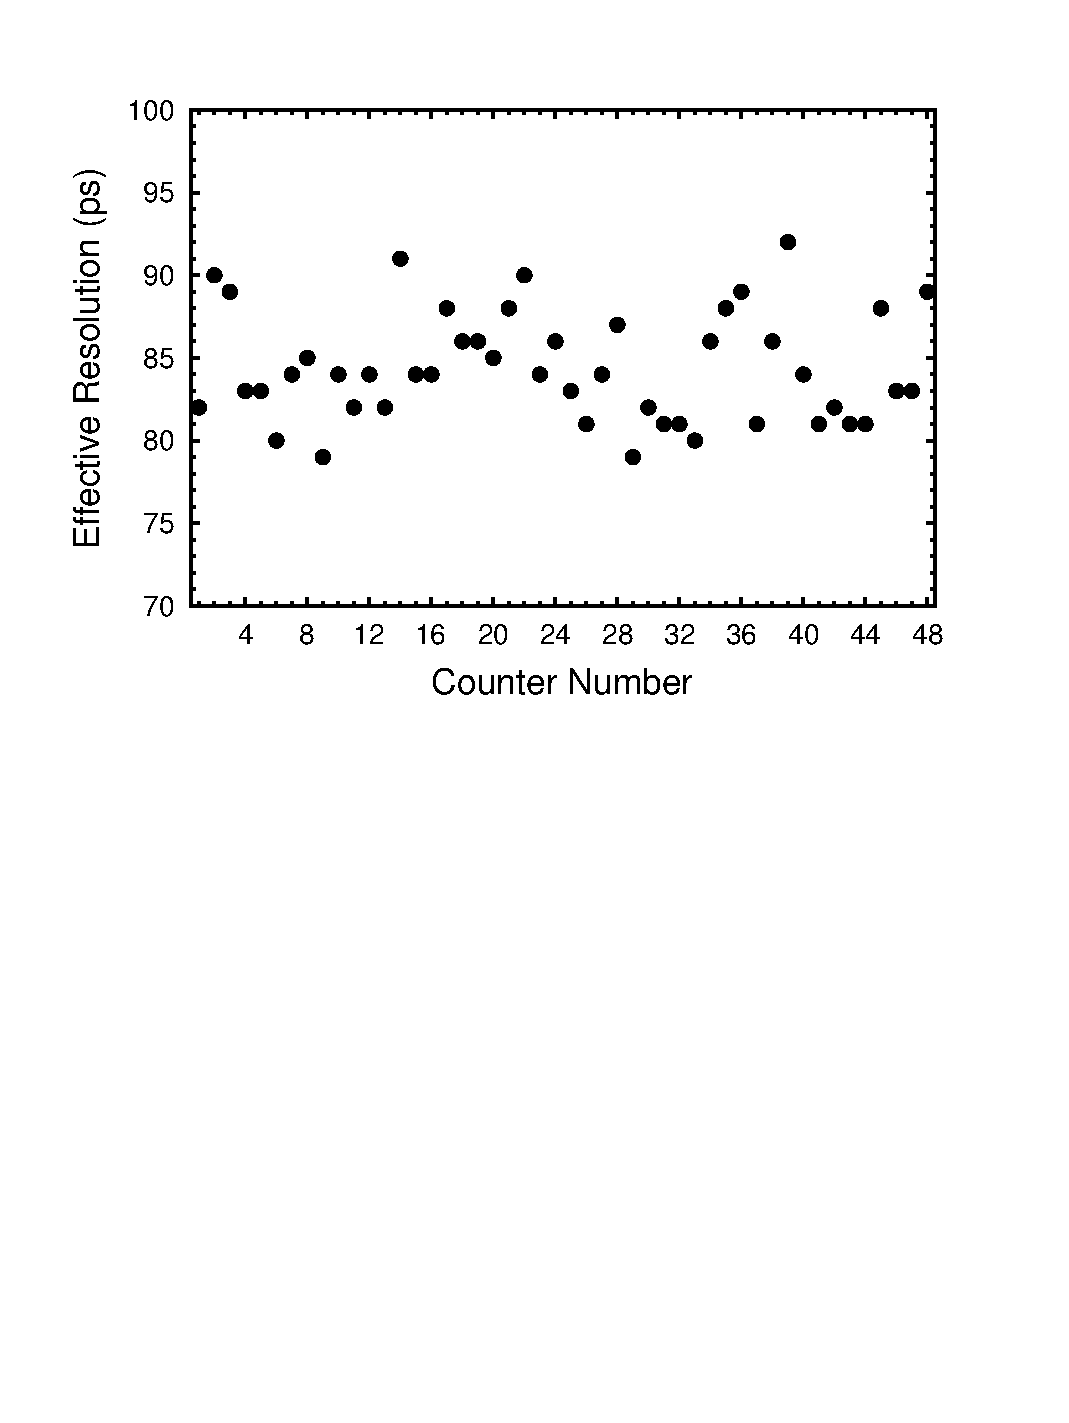
\includegraphics[width=0.5\textwidth,natwidth=610,natheight=642]{pics/res-beam.pdf}}}
\end{picture} 
\caption{The measured effective time resolution (ps) vs. counter number for each of the CTOF counters
from beam data for a 10.6~GeV electron beam incident upon a liquid-hydrogen target with the solenoid
at full field.}
\label{eff-tres}
\end{figure}
%%%%%%%%%%%%%%%%%%%%%%%%%%%%%%%%%%%%%%%%%%%%%%%%%%%%%%%%%

Note that the CTOF counter time resolutions shown in Fig.~\ref{eff-tres} are referred to effective time
resolutions as they include additional smearing effects beyond that included in the resolutions discussed and
shown in Section~\ref{sec-bench} determined from the cosmic ray test stand. The contributions from all
non-CTOF sources to the effective resolution effectively adds $\sim$50~ps of smearing in quadrature with
the intrinsic CTOF counter resolution.

\subsubsection{Counter Hit Times}
\label{cluster}

After completion of each of the timing calibration steps discussed in this section, the CTOF hit time associated
with a matched charged particle track can be determined. Putting all of the timing corrections together, the
track hit time reconstructed from the readout of the upstream and downstream PMTs are given by:
\begin{multline}
  t_{U,D} = (CONV \cdot TDC_{U,D}) \mp \frac{C_{UD}}{2} + \\ C_{RF} + C_{p2p} + \frac{\delta t_{hpos}}{2},
\end{multline}

\noindent
where $CONV$ is the TDC channel to time conversion factor, $TDC$ is the measured TDC value relative
to the trigger signal, $C_{UD}$ is the time shift to center the TDC difference distribution relative to the
track coordinate about 0, $C_{RF}$ and $C_{p2p}$ are the time shifts to align all of the counter times
with respect to the RF and to each other, respectively, and $\delta t_{hpos}$ is the hit position dependent
time correction (with half of the correction added to each of $t_U$ and $t_D$).

The actual hit time associated with the track has to be corrected for the propagation time of the light from
the track hit point on the counter to the PMT. The final reported track hit time is then the average of
the upstream and downstream corrected PMT time. Another aspect of the CTOF hit reconstruction is associated
with tracks that cross through multiple CTOF bars as they pass into or through the barrel. These are referred
to a hit clusters. Full details on the CTOF reconstruction algorithms, including hit times, and the hit clustering
and matching algorithms are provided in Refs.~\cite{recon-nim,ctof-recon}.

\subsection{Beam Performance}  
\label{sec:beam}

The first in-beam characterization of the CTOF system took place during the Dec. 2017 to Feb. 2018
CLAS12 Engineering Run and subsequently during the first physics production running periods that took place
from Mar. - May 2018 and Sep. - Dec. 2018. During these periods the performance of the CTOF system was
tested at different beam energies (2.2, 6.5, 7.5, 10.6~GeV), different solenoid magnetic field strengths and
polarities (from 0 field to full field), and over a range of beam-target luminosities up to the nominal CLAS12
luminosity of $1 \times 10^{35}$~cm$^{-2}$s$^{-1}$. In this section the measured scaler rates and PMT currents
as a function of beam current are presented, as well as the reconstruction results and particle identification
capabilities relative to the system specifications based on the current system reconstructions and calibrations.

\subsubsection{CTOF Rates and PMT Currents}

The count rates during beam operations can be viewed during data taking using the scalers associated
with the FADCs. The threshold applied for these scalers is set at 1~MeV. During a beam current scan
with a 10.6~GeV electron beam incident upon the 5-cm long liquid-hydrogen target from 5~nA to 75~nA
(with 75~nA corresponding to the nominal design luminosity for CLAS12) and the solenoid at its full nominal
current, the average count rate in the different CTOF counters was studied. The results shown in
Fig.~\ref{ctof-rates} display a reasonably linear behavior with the average rate at full luminosity
$<$500~kHz. The rates in the downstream PMTs are roughly a factor of two larger than in the upstream
PMTs. Part of this difference is due to the fact that the events seen by the CTOF are predominantly
focused at the downstream end of the counters. Therefore the average path length for light to travel is
longer to the upstream PMTs and a rate difference is expected due to light attenuation effects. However,
another important contribution is believed to be due to incident radiation on the downstream light guides from
splash-back from the entrance to the beamline M{\o}ller cone and the copious $\pi^0 \to \gamma \gamma$
conversions in the region about the target. This radiation generates significant Cherenkov light in the light
guides that is seen by the downstream PMTs and not by the upstream PMTs.

%%%%%%%%%%%%%%%%%%%%%%%%%%%%%%%%%%%%%%%%%%%%%%%%%%%%%%%%%
\begin{figure}[htbp]
\vspace{2.1cm}
\begin{picture}(50,50) 
\put(27,-52)
{\hbox{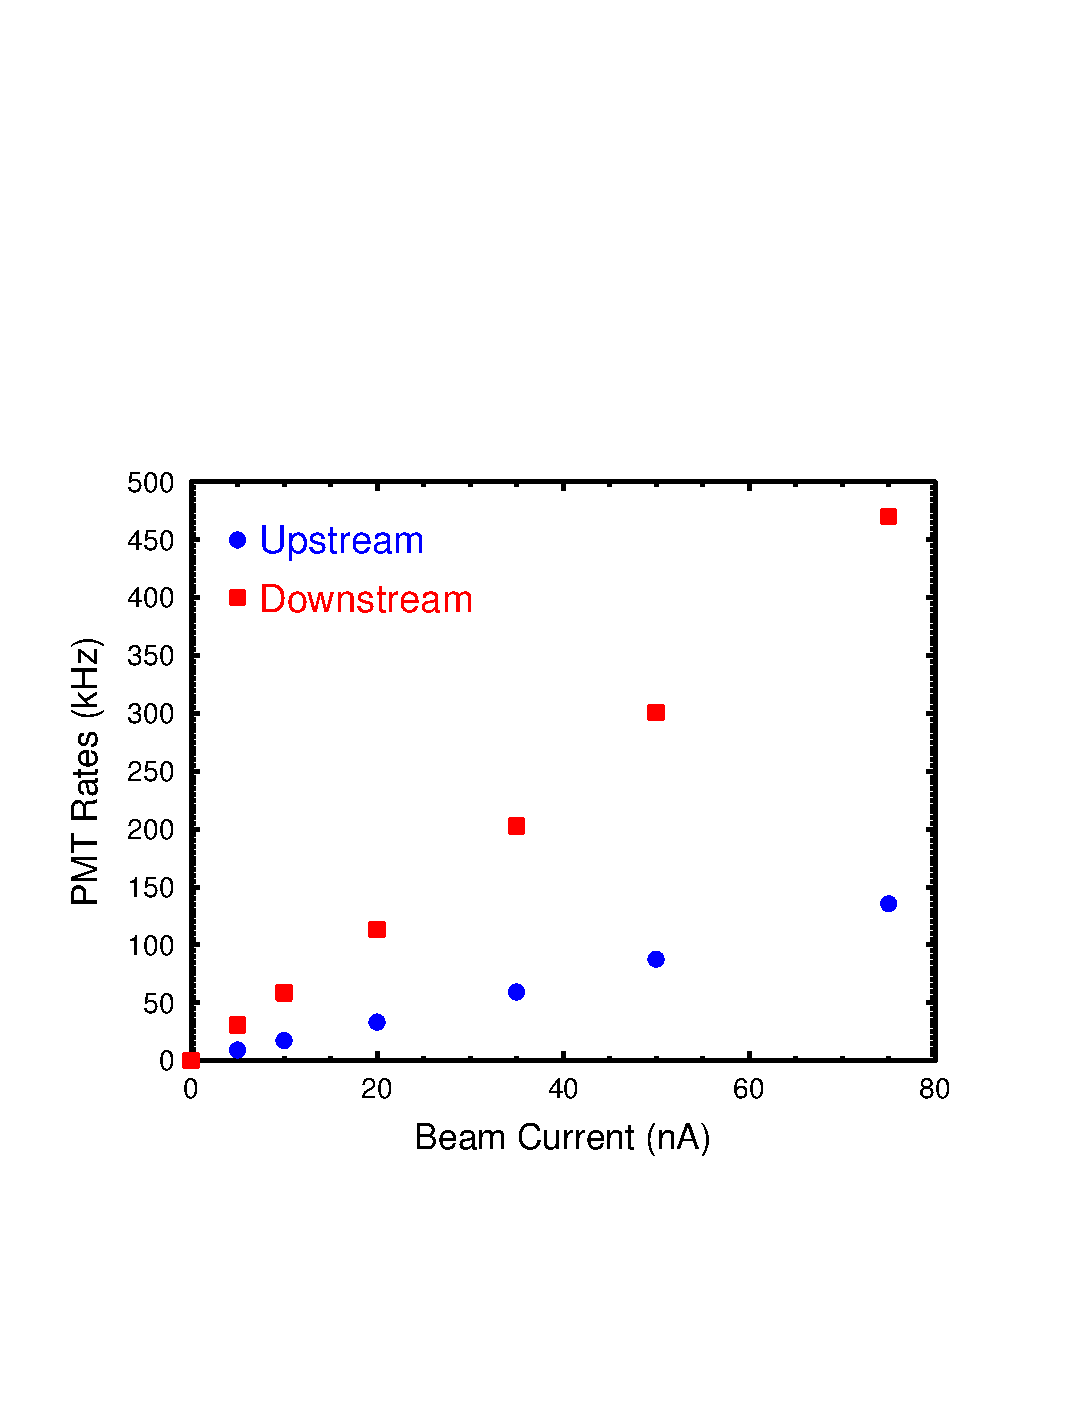
\includegraphics[width=0.45\textwidth,natwidth=610,natheight=642]{pics/rates-ctof.pdf}}}
\end{picture} 
\caption{CTOF counter rates (kHz) for 10.6~GeV electrons on a liquid-hydrogen target with the
solenoid at its full nominal current as a function of beam current (nA) with a 1~MeV energy threshold.
The nominal operating luminosity of CLAS12 of $1 \times 10^{35}$~cm$^{-2}$s$^{-1}$ corresponds to
a beam current of $\sim$75~nA.}
\label{ctof-rates}
\end{figure}
%%%%%%%%%%%%%%%%%%%%%%%%%%%%%%%%%%%%%%%%%%%%%%%%%%%%%%%%%

Studies using the CLAS12 Geant4 Monte Carlo suite called GEMC~\cite{sim-nim} at the full nominal
luminosity with an 11~GeV electron beam with the solenoid at full field, indicate that the total integrated
rates (hadronic and neutral) for particles that deposit energy greater than 1~MeV in the counters is
$\sim$100~kHz/counter and the nominal PMT currents for all incident radiation on the counter (i.e. with
no energy threshold) are $\sim$30-40~$\mu$A~\cite{ctof-cn2018}. Figure~\ref{ctof-mc} shows the
Monte Carlo results for the CTOF counter rates as a function of track momentum for different particle
species. The results of these studies show that for each CTOF counter the incident rate of all charged and
neutral particles is 4~MHz, of which $\sim$97\% is photons and leptons. With a 1~MeV energy deposition
threshold in the CTOF counters to match that applied to the hardware, the rate of charged and neutral
particles is $\sim$130~kHz/counter (equal upstream and downstream), half of which is leptons + photons
and half is hadronic. The prediction for the upstream PMTs matches well what is seen in direct measurements
during beam operations. However, the prediction for the downstream PMTs is a factor of three lower than the
direct measurements. This is likely due to the fact that in the simulation the CTOF light guides are not active
materials in which events that generate Cherenkov light in the light guides (see remarks above) are modeled
or included.

%%%%%%%%%%%%%%%%%%%%%%%%%%%%%%%%%%%%%%%%%%%%%%%%%%%%%%%%%
\begin{figure}[htbp]
\vspace{2.6cm}
\begin{picture}(50,50) 
\put(23,126)
{\hbox{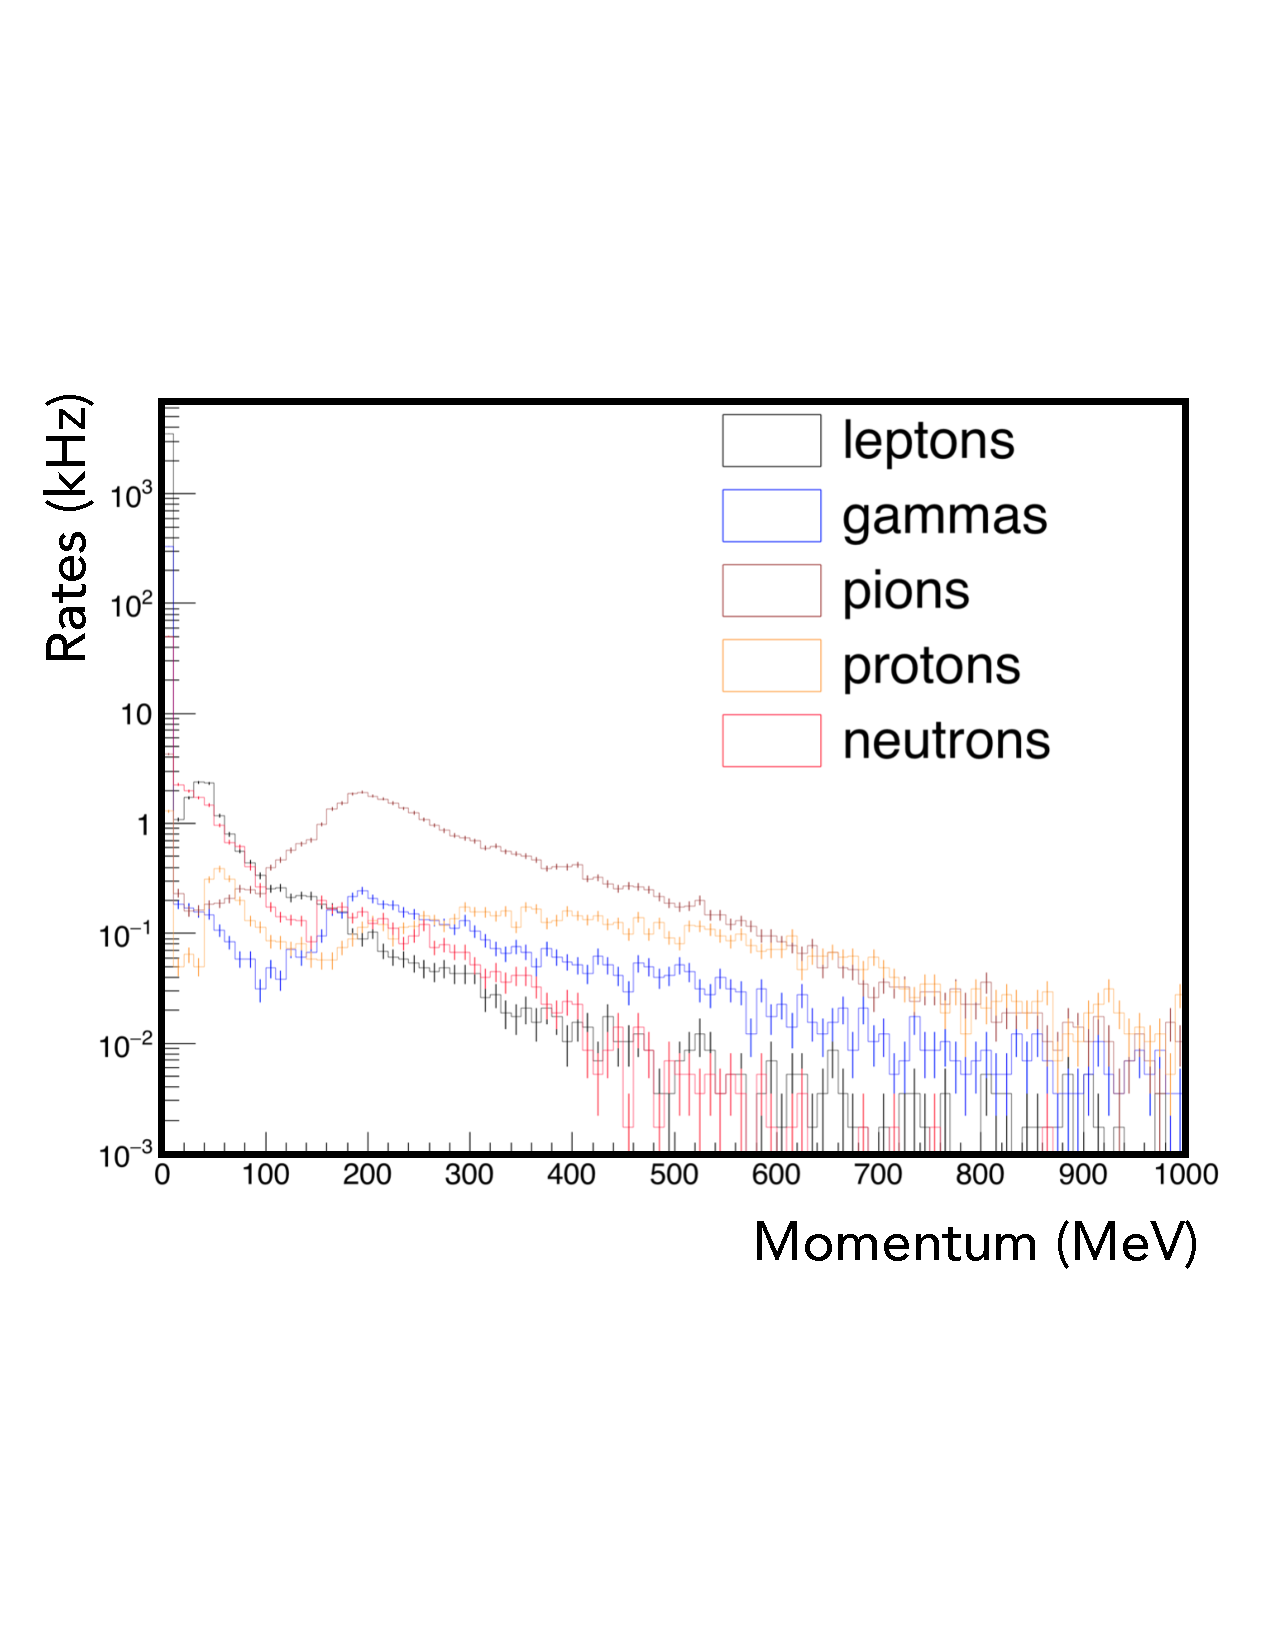
\includegraphics[width=0.30\textwidth,natwidth=610,natheight=642,angle=-90]{pics/ctof-mc-plot.pdf}}}
\end{picture} 
\caption{CLAS12 Monte Carlo calculations for 11 GeV electrons on a liquid-hydrogen target at a luminosity
of $1 \times 10^{35}$~cm$^{-2}$s$^{-1}$ showing CTOF rates per counter as a function of particle
momentum for leptons (black), photons (blue), charged pions (brown), protons (gold), and neutrons (red).
The simulations were done with the solenoid at its full nominal current.}
\label{ctof-mc}
\end{figure}
%%%%%%%%%%%%%%%%%%%%%%%%%%%%%%%%%%%%%%%%%%%%%%%%%%%%%%%%%

Practically, it is not the event rate that defines the operational limit of the CTOF system, but the PMT
anode currents, which are limited to $\sim$200~$\mu$A (see Section~\ref{divider}). The average
PMT current is directly proportional to the average number of photoelectrons $\langle N_{phe} \rangle$
created at the photocathode by the scintillation light and the average incident charged particle event rate
$\langle R \rangle$. This current can be expressed as:

\begin{equation}
\langle i_{PMT} \rangle = \langle N_{phe} \rangle \cdot Q_e \cdot G \cdot \langle R \rangle,
\end{equation}

\noindent
where $Q_e = 1.6 \times 10^{-19}$ C/e is the electron charge, $G$ is the PMT gain, and $R$ is the rate
per bar. Using the expected photoelectron statistics discussed in Section~\ref{sec:npe} at a PMT gain
of 1$\times$10$^6$, the simulations estimated PMT currents of 30-40~$\mu$A at full nominal CLAS12
luminosity. Direct measurements in beam of the PMT anode currents were made as a function of beam
current as shown in Fig.~\ref{pmt-currents}. The measurements are about two times larger than
expectations. The discrepancy is most likely due to the fact that the sampled PMT (randomly chosen on
the upstream end of CTOF) was operating at a gain above 1$\times$10$^6$.

%%%%%%%%%%%%%%%%%%%%%%%%%%%%%%%%%%%%%%%%%%%%%%%%%%%%%%%%%
\begin{figure}[htbp]
\vspace{2.0cm}
\begin{picture}(50,50) 
\put(27,-53)
{\hbox{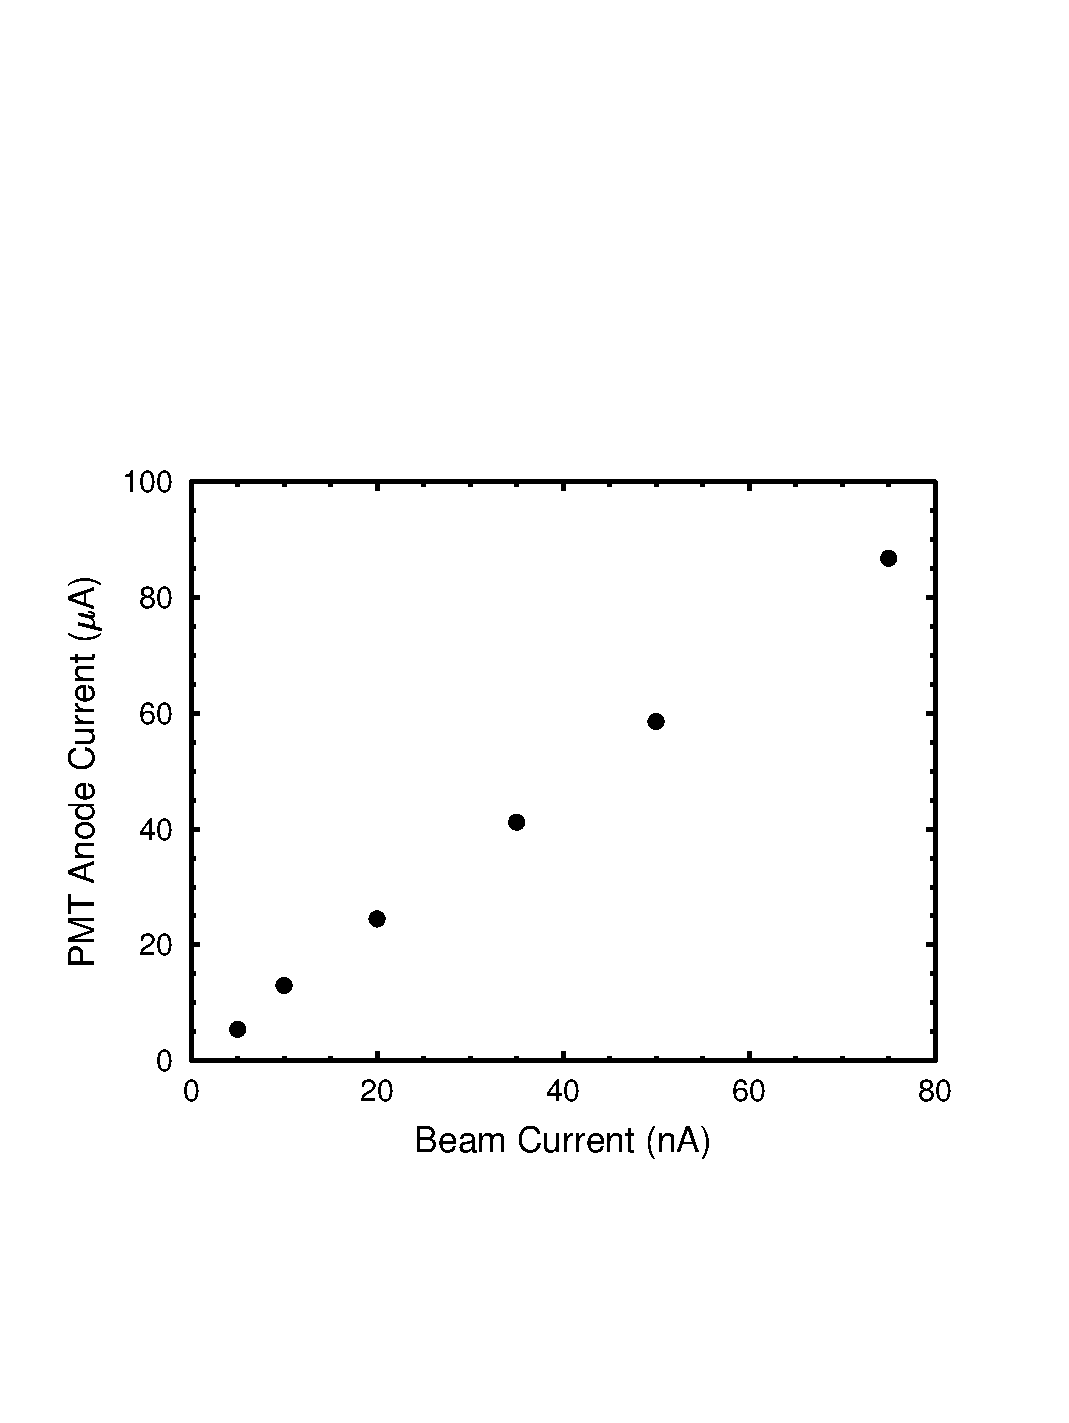
\includegraphics[width=0.46\textwidth,natwidth=610,natheight=642]{pics/full-ctof.pdf}}}
\end{picture} 
\caption{Measurements of the PMT anode current ($\mu$A) for a representative upstream CTOF PMT
as a function of beam current (nA) with a 10.6~GeV electron incident upon a 5~cm liquid-hydrogen target
and the solenoid at full field.}
\label{pmt-currents}
\end{figure}
%%%%%%%%%%%%%%%%%%%%%%%%%%%%%%%%%%%%%%%%%%%%%%%%%%%%%%%%%

\subsubsection{Reconstruction Results}

Particle identification in the Central Detector of CLAS12 relies heavily on the combination of measured
charged particle momenta and the flight time from the target to the respective CTOF counters. The
vertex time is determined with respect to the accelerator RF, modulo the RF period $T_{RF}$. The beam
bucket for each event is identified using the flight time of scattered electrons or high momentum pions
detected in the CLAS12 Forward Detector traced back to the interaction point. The FTOF resolution of
$< 200$~ps~\cite{ftof-nim}  allows clear selection of the correct beam bucket. In Fig.~\ref{ctof-pid}(right)
we show the distributions of mass squared for all reconstructed positively and negatively charged hadrons in
CTOF without any kinematic cuts other than those imposed by the detector acceptance for the data taken
with a 10.6~GeV electron beam incident upon a liquid-hydrogen target and after initial calibrations of the
CTOF system. A clear separation of pions and protons can be seen from these data. 

%%%%%%%%%%%%%%%%%%%%%%%%%%%%%%%%%%%%%%%%%%%%%%%%%%%%%%%%%
\begin{figure}[htbp]
\vspace{4.2cm}
\begin{picture}(50,50) 
\put(12,-65)
{\hbox{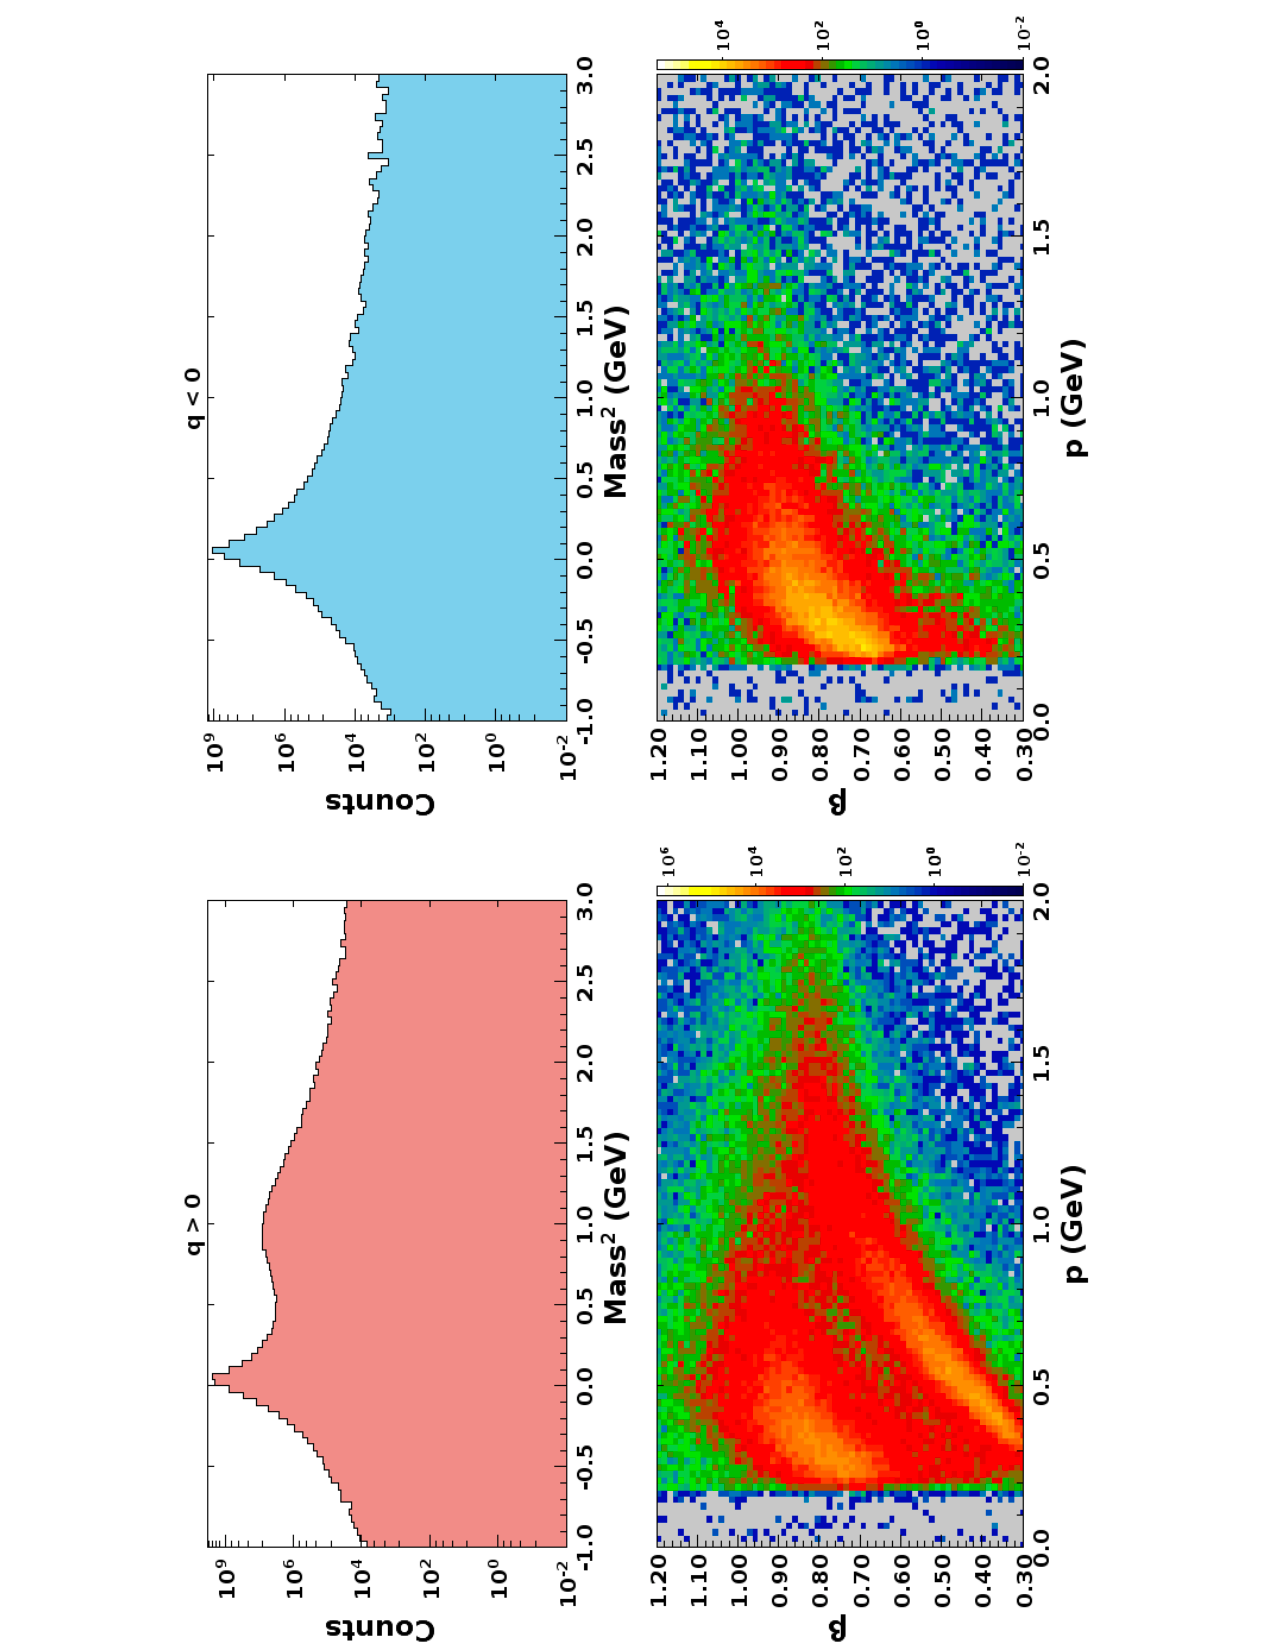
\includegraphics[width=0.45\textwidth,natwidth=610,natheight=642]{pics/ctof-pid.pdf}}}
\end{picture} 
\caption{Reconstructed $\beta$ vs. momentum (GeV) (left) and mass squared (GeV$^2$) (right)
distributions for positively charged particles (top) and negatively charged particles (bottom) for
all CTOF counters from beam data with a 10.6~GeV electron incident upon a liquid-hydrogen target.
The overlaid curves show the expected locations of charged pions ($\pi$), kaons ($K$), and
protons ($p$).}
\label{ctof-pid}
\end{figure}
%%%%%%%%%%%%%%%%%%%%%%%%%%%%%%%%%%%%%%%%%%%%%%%%%%%%%%%%

Plots of velocity versus momentum are shown in Fig. \ref{ctof-pid}(left) for positively and negatively charged
particles, displaying the overall particle identification possible with this detector through the separation
of the different particle species. These distributions qualitatively show the particle separation for $\pi/K$,
$\pi/ p$, and $K/p$ vs. momentum as required by the system specifications in Section~\ref{sec:overview}
and Table~\ref{spec-table}. Note that without additional reaction-specific cuts on event selection, charged
kaons are difficult to see clearly in these distributions due to their lower cross sections and production
dynamics. The overlaid curves show the expected values of $\beta$ vs. $p$ for the different particle species.
Slight differences between the data and expectations reflect the current quality of Central Detector calibrations
and reconstruction.

%%%%%%%%%%%%%%%%%%%%%%%%%%%%%%%%%%%%%%%%%%%%%%%%%%%%%%%%%
\begin{figure}[htbp]
\vspace{4.1cm}
\begin{picture}(50,50) 
\put(15,-65)
{\hbox{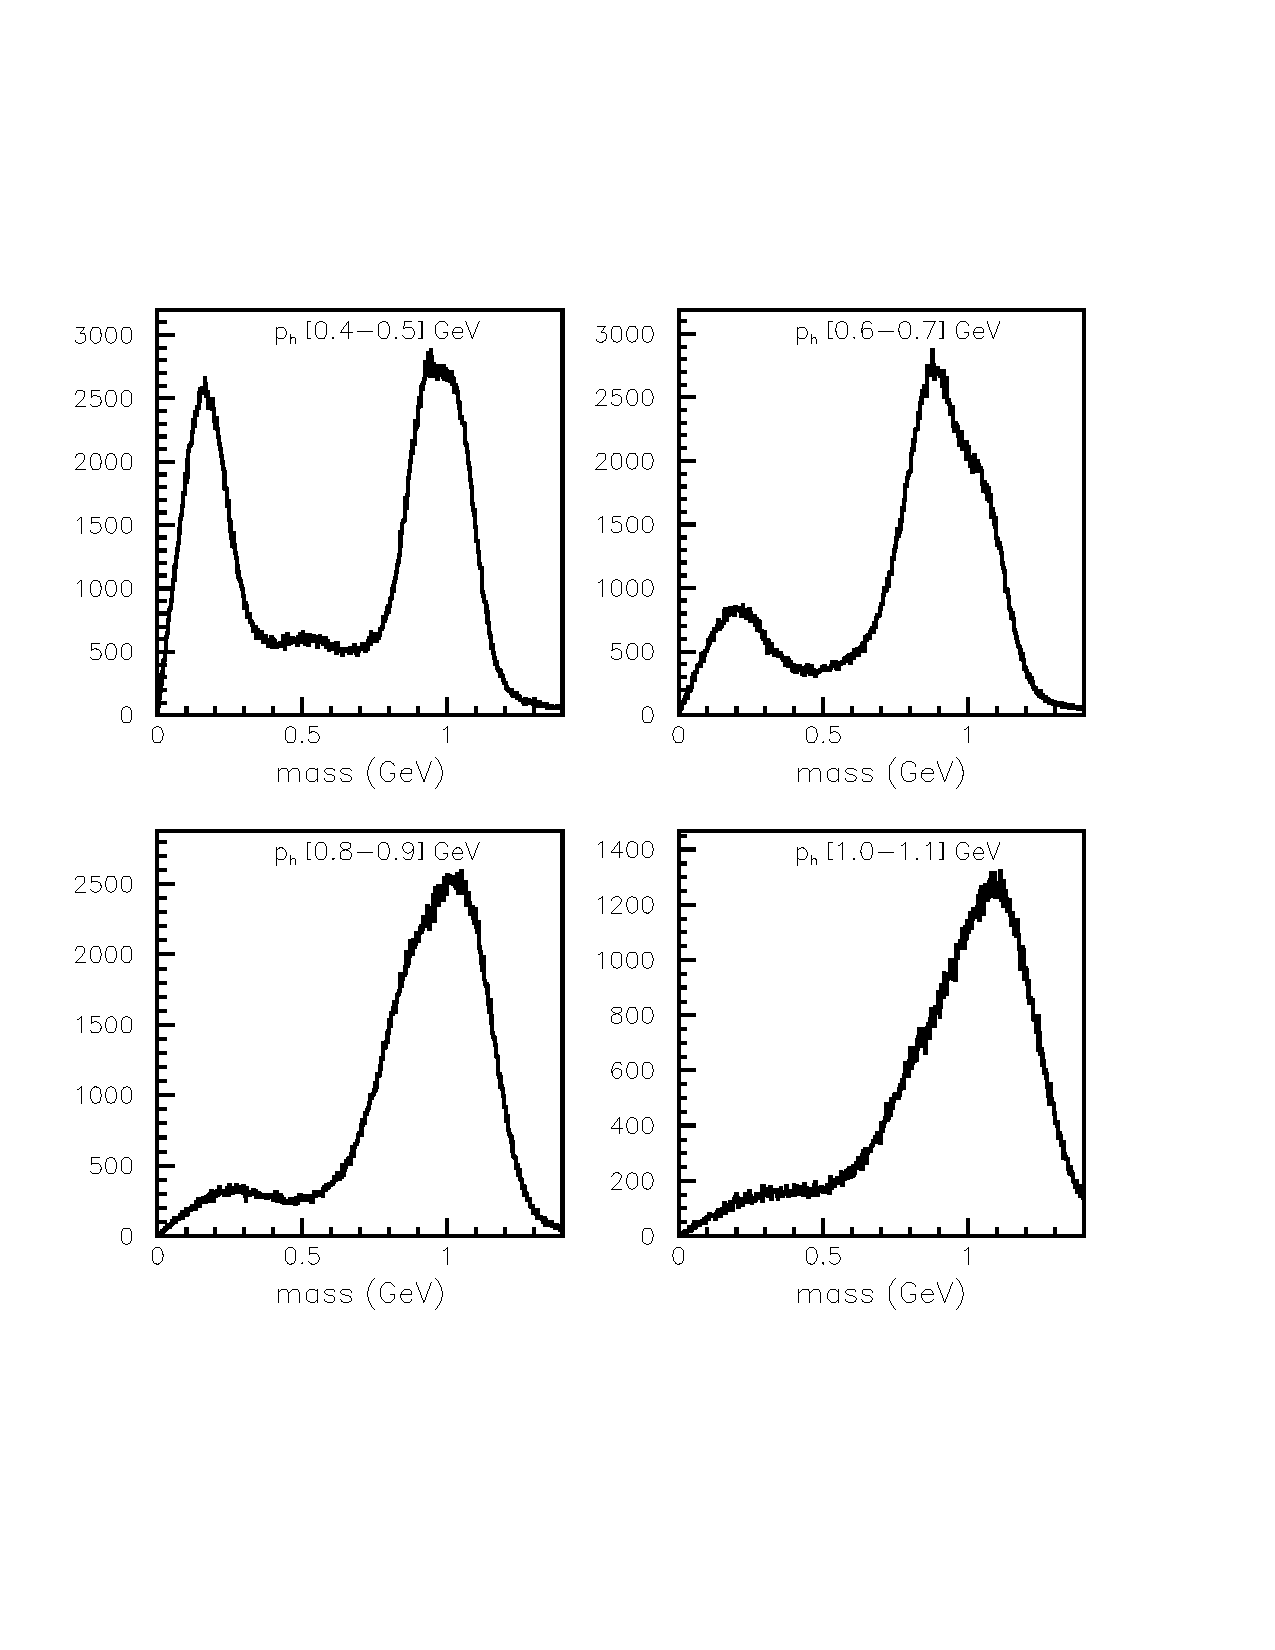
\includegraphics[width=0.45\textwidth,natwidth=610,natheight=642]{pics/ctof-mass.pdf}}}
\end{picture} 
\caption{Reconstructed mass (GeV) for positively charged particles from the timing in CTOF counters from
beam data with a 7.5-GeV electron beam incident on a liquid-hydrogen target. The data are sorted into four
bins in hadron momentum as indicated and are based on the current CLAS12 detector calibrations, detector
alignments, and event reconstruction.}
\label{ctof-mass}
\end{figure}
%%%%%%%%%%%%%%%%%%%%%%%%%%%%%%%%%%%%%%%%%%%%%%%%%%%%%%%%

To connect the particle identification limits from the CTOF system with those detailed in
Section~\ref{sec:overview}, Fig.~\ref{ctof-mass} shows the reconstructed mass for positively charged
particles in the Central Detector of CLAS12 based on initial calibrations of the CTOF system. In order to
avoid timing resolution effects that would truncate the mass squared distribution when taking the square
root, Fig.~\ref{ctof-mass} plots the reconstructed hadron mass squared using:

\begin{equation}
M^2 = p_h^2 \cdot \frac{1.-\beta^2}{\beta^2},~~~~\beta=\frac{P_L}{t_p c},
\end{equation}

\noindent
where $p_h$ is the particle momentum determined by the central tracking system, $P_L$ is the hadron
path length from the event vertex in the target to the CTOF system, $t_p= \bar{t}_{hit} - t_{ST}$ is
the particle flight time over $P_L$, and $c$ is the speed of light. Fig.~\ref{ctof-mass} shows the mass
squared distributions for several bins in hadron momentum from 0.4~GeV to 1.0~GeV. Even with the current
state of CLAS12 detector calibrations, detector alignment, and knowledge of the solenoid magnetic field,
these distributions show reasonable separation between $\pi/K$ up to about 0.5~GeV and separation of
$\pi$ from $p$ to about 1~GeV, in reasonable agreement with the limits defined in Table~\ref{spec-table}.
Improvements in the CTOF and central tracking calibrations and detector alignment are still expected
should give improved particle identification and separation of the different charged hadron species to
higher momentum in the future.

\section{Summary}
\label{sec:summary}

We have designed and built a time-of-flight system for the CLAS12 Central Detector in Hall~B 
at Jefferson Lab known as the Central Time-of-Flight or CTOF detector. This system consists 
of 48 90-cm-long scintillation bars of a wedge-shaped cross section that form a hermetic barrel
at a radius of 25~cm from the beamline. As this system is positioned inside of a 5-T superconducting
solenoid, the light is delivered to the PMTs through long light guides to allow the PMTs to be positioned
in reduced field regions where a dynamic multi-layer shield system reduces the magnet fringe fields to
the level of 0.2~G at the PMT photocathode. The scintillation bars are read out at each end. The
detector was designed to have an intrinsic time resolution of about 65~ps and an effective time resolution
of 80~ps, and this level of performance has been achieved. With these time resolutions the CTOF system
can separate $\pi/K$ to 0.58~GeV, $K/p$ to 0.93~GeV, and $\pi/p$ to 1.14~GeV with 3$\sigma$
separation with up to an order of magnitude difference in the relative yields.  The specifications are
sufficient to meet the particle identification requirements in the central direction for the full CLAS12
physics program. The performance of the CTOF system was verified in extensive bench studies in our
cosmic ray test stand, as well as after installation in the first beam runs with the CLAS12 system in the
period from Dec. 2017 to May 2018 and from Sep. to Dec. 2018. 

\section*{Acknowledgments}

We benefited greatly from useful discussions with and assistance from Sergey Boyarinov, Chris
Cuevas, Ralf Gothe, Chris Keith, Eugene Pasyuk, Cole Smith, Elton Smith, Maurizio Ungaro, and
Veronique Ziegler. We thank the Hall~B technical crew for their efforts during counter installation,
the JLab Detector Support Group for contributing to component assembly and testing, and members of
the Hall~B Engineering and Design Groups that contributed to the detector advancement during the
design stage. This material is based upon work supported by the U.S. Department of Energy, Office of
Science, Office of N. Finally, we thank the students and post-docs who contributed their time and energy
during the research and development phase of this project. This material is based upon work supported in
part by the U.S. Department of Energy, Office of Science, Office of Nuclear Physics under contract
DE-AC05- 06OR23177.

\begin{thebibliography}{99}

\bibitem{overview-nim}
V.D. Burkert {\it et al.}, {\it ``The CLAS12 Spectrometer at Jefferson Laboratory''}, to be published in Nucl.
Inst. and Meth. A, (2020). (see this issue)

\bibitem{htcc-nim}
Y. Sharabian {\it et al.}, {\it ``The CLAS12 High Threshold Cherenkov Counter''}, to be published in Nucl.
Inst. and Meth. A, (2020). (see this issue)
  
\bibitem{cnd-nim}
P. Chatagnon {\it et al.}, {\it ``The CLAS12 Central Neutron Detector''}, to be published in Nucl. Inst.
and Meth. A, (2020). (see this issue)
  
\bibitem{svt-nim}
M. A. Antonioli {\it et al.}, {\it ``The CLAS12 Silicon Vertex Tracker''}, to be published in Nucl. Inst.
and Meth. A, (2020). (see this issue)

\bibitem{mm-nim}
F. Bossu {\it et al.}, {\it ``The CLAS12 MicroMegas Tracker''}, to be published in Nucl. Inst.
and Meth. A, (2020). (see this issue)
  
\bibitem{clas-nim}
B.A. Mecking {\it et al.}, Nucl. Inst. and Meth. {\bf A503}, 513 (2003).

\bibitem{trigger-nim}
B. Raydo {\it et al.}, {\it ``The CLAS12 Trigger System''}, to be published in Nucl. Inst. and Meth. A, (2020).
(see this issue)

\bibitem{baturin-2009}
V. Baturin {\it et al.}, {\it ``Time Resolution Measurements with the Final Prototype for the 
CLAS12 Central TOF Detector''}, CLAS-Note 2009-001, (2009).\\
https://misportal.jlab.org/ul/Physics/Hall-B/clas/\\ viewFile.cfm/2009-001.pdf?documentId=549

\bibitem{geom-note}
V. Baturin and D.S. Carman, {\it ``Central Time-of-Flight Geometry for CLAS12''}, CLAS12-Note 
2016-001, (2016).
https://misportal.jlab.org/mis/physics/clas12/\\ viewFile.cfm/2016-001.pdf?documentId=25

\bibitem{eljen-ref}
Eljen EJ-200 Data Sheet,\\
https://eljentechnology.com/images/products/\\
data\_sheets/EJ-200\_EJ-204\_EJ-208\_EJ-212.pdf

\bibitem{eljen-guide}
Eljen Technology Scintillator Polishing Guide,\\
http://www.eljentechnology.com/images/technical-library/Plastic\_Polishing.pdf

\bibitem{barbosa06}
F. Barbosa {\it et al.}, {\it ``Status and Further Steps Towards the CLAS12 ``Start''-Counter''},
CLAS-Note 2006-011, (2006).\\
https://misportal.jlab.org/ul/Physics/Hall-B/clas/viewFile.cfm/2006-011.pdf?documentId=278

\bibitem{guide7} 
T. Massam, Guide7, {\it ``A General Program for Evaluating the Properties of Scintillation and
Cherenkov Counter Optical Systems''}, CERN Report EP-76-21, (1976),

\bibitem{r2083-ref}  
Hamamatsu R2083 PMT, \\
http://www.hamamatsu.com/us/en/R2083.html

\bibitem{ham-schem}
Hamamatsu H2431 Assembly, \\
http://www.hamamatsu.com/resources/pdf/\\ etd/PMT\_TPMZ0002E.pdf

\bibitem{popov}
V. Popov, Nucl. Inst. and Meth.A {\bf 505}, 316 (2003).

\bibitem{baturin12}
V. Baturin {\it et al.}, Nucl. Inst. and Meth. A {\bf 664}, 11 (2012).

\bibitem{cn2015-003} 
V. Baturin and D.S. Carman, {\it ``Design and Performance Tests of the Dynamical Magnetic Shields 
for the CLAS12 Central Time-of-Flight Detector''}, CLAS12-Note 2015-003.\\
https://misportal.jlab.org/mis/physics/clas12/\\
viewFile.cfm/2015-003.pdf?documentId=19

\bibitem{shield-test} 
D.S. Carman, G. Asryan, and A. Ni, {\it ``Central Time-of-Flight Magnetic Shield Performance Studies''},
CLAS12-Note 2015-004, (2015).\\
https://misportal.jlab.org/mis/physics/clas12/\\
viewFile.cfm/2015-004.pdf?documentId=20

\bibitem{ctof-wrapping} 
D.S. Carman, {\it ``Central Time-of-Flight Counter Wrapping Procedures''}, CLAS12-Note 2016-002, (2016).\\
https://misportal.jlab.org/mis/physics/clas12/\\
viewFile.cfm/2016-002.pdf?documentId=26

\bibitem{ctof-sh-assy} 
D.S. Carman, {\it ``Central Time-of-Flight Magnetic Shield Attachment Procedures''}, CLAS12-Note 
2016-003, (2016).\\
https://misportal.jlab.org/mis/physics/clas12/\\
viewFile.cfm/2016-003.pdf?documentId=27

\bibitem{daq-nim}
S. Boyarinov {\it et al.}, {\it ``The CLAS12 Data Acquisition System''}, to be published in Nucl. Inst.
and Meth. A, (2020). (see this issue)
  
\bibitem{fadc-manual}
JLab 250~MHz FADC Manual, https://www.jlab.org/\\ Hall-B/ftof/manuals/FADC250UsersManual.pdf
  
\bibitem{recon-nim}
V. Ziegler {\it et al.}, {\it ``CLAS12 Software Framework and Event Reconstruction''}, to be published in Nucl. Inst.
and Meth. A, (2020). (see this issue)
  
\bibitem{epics}
EPICS (Experimental Physics and Industrial Control System), http://www.aps.anl.gov/epics

\bibitem{dsc-cn2016-009}
D.S. Carman, {\it ``Central Time-of-Flight System Bench Testing Results''},
CLAS12-Note 2016-009, (2016).\\
https://misportal.jlab.org/mis/physics/clas12/\\ viewFile.cfm/2016-009.pdf?documentId=49

\bibitem{ctof-calib}
D.S. Carman, {\it ``Description of the Calibration Algorithms for the CLAS12 Central Time-of-Flight System''},
CTOF internal note, \\
https://www.jlab.org/Hall-B/ctof/notes/ctof\_calib.pdf

\bibitem{ftof-nim}
D.S. Carman {\it et al.}, {\it ``The Forward Time-of-Flight System for CLAS12''}, to be published in Nucl.
Inst. and Meth. A, (2020). (see this issue)

\bibitem{ctof-recon}
D.S. Carman, {\it ``Central Time-of-Flight Reconstruction for CLAS12''}, CTOF internal note, \\
https://www.jlab.org/Hall-B/ctof/notes/ctof-recon.pdf

\bibitem{sim-nim}
M. Ungaro {\it et al.}, {\it ``The CLAS12 Geant4 Simulation''}, to be published in Nucl. Inst.
and Meth. A, (2020). (see this issue)
  
\bibitem{ctof-cn2018}
V. Burkert, D.S. Carman, L.C. Smith, and M. Ungaro, {\it ``Study of Tungsten Shielding Before CTOF to Limit
its PMT Currents''}, CLAS12-Note 2018-006, (2018).\\
https://misportal.jlab.org/mis/physics/clas12/\\ viewFile.cfm/2018-006.pdf?documentId=60

\end{thebibliography}

\end{document}
